%%%%%%%%%%%%%%%%%%%%%%%%%%%%%%%%%%%%%%%%%%%%%%%%%%%%%%%%%%%%%%%%%%%%%%
%%  
%%  UT-THESIS.TEX
%%  Copyright (c) 1998-2000 by Francois Pitt
%%  Last Update: 2000 February 20
%%  
%%  Skeleton LaTeX2e file for the preparation of theses at UofT;
%%  conforms to the School of Graduate Studies' guidelines of 07/97.
%%  To be used in conjunction with class file `ut-thesis.cls', whose
%%  features it illustrates.
%%  
%%%%%%%%%%%%%%%%%%%%%%%%%%%%%%%%%%%%%%%%%%%%%%%%%%%%%%%%%%%%%%%%%%%%%%
%%  
%%  This file is distributed in the hope that it will be useful but
%%  without any warranty (without even the implied warranty of
%%  fitness for a particular purpose).  For a description of this
%%  file's purpose, and instructions on its use, see below.
%%  
%%  Feel free to copy and redistribute this file, as long as this
%%  copyright notice remains intact and this file is distributed
%%  along with the companion file `ut-thesis.cls'.
%%  
%%  (Thanks to Robert Bernecky for his suggestions on improving the
%%  usefulness and readability of this file.)
%%  
%%  Send all bugs, questions, comments, suggestions, etc. to the
%%  author, at <fpitt_AT_cs_DOT_utoronto_DOT_ca>.
%%  
%%%%%%%%%%%%%%%%%%%%%%%%%%%%%%%%%%%%%%%%%%%%%%%%%%%%%%%%%%%%%%%%%%%%%%
%%  
%%  SUMMARY OF FEATURES:
%%  
%%  To comment out parts of a file, use the macro \ignore{...}
%%  around the entire block of text you want to ignore.
%%  
%%  To explicitly set the pagestyle of any inserted blank page when
%%  \cleardoublepage occurs, use one of \clearemptydoublepage or
%%  \clearplaindoublepage instead.
%%  
%%  For single-spaced quotes or quotations, use the `longquote' and
%%  `longquotation' environments.  For single-spaced, 1 1/2-spaced,
%%  or double-spaced paragraphs, use one of the environments
%%  `singlespaced', `oneandahalfspaced', or `doublespaced'.  More
%%  generally, for paragraphs with a line spacing of `n', use
%%  `\begin{newspacing}{n}...\end{newspacing}'.
%%  
%%  All other environments, commands, and options provided by the
%%  `ut-thesis' class will be described below, at the point where
%%  they should appear in the document.
%%  
%%  See the companion file `ut-thesis.cls' for more details.
%%  
%%%%%%%%%%%%%%%%%%%%%%%%%%%%%%%%%%%%%%%%%%%%%%%%%%%%%%%%%%%%%%%%%%%%%%


%%%%%%%%%%%%         PREAMBLE         %%%%%%%%%%%%

%% Default settings format a final copy (12pt font, single-sided,
%% double-spaced, normal margins, single-spaced notes).  For a rough
%% copy (10pt font, double-sided, double-spaced, normal margins, with
%% the word "DRAFT" printed at each corner of every page), use the
%% `draft' option.  The default line spacing can be changed with one
%% of the following options: `singlespaced', `oneandahalfspaced', or
%% `doublespaced'.  The notes are always single-spaced by default, but
%% can be made to have the same spacing as the rest of the document by
%% using the option `spacednotes'.  The size of the margins can be
%% changed with one of the following options: `narrowmargins' (1 1/4"
%% left, 3/4" others), `normalmargins' (1 1/4" left, 1" others),
%% `widemargins' (1 1/4" all), `extrawidemargins' (1 1/2" all).  Any
%% other standard option for the `report' document class can be used
%% to override the default or draft settings.

%% ***   Add any desired options.   ***
\documentclass{ut-thesis}

%% ***   Add \usepackage declarations here.   ***


%% The line spacing of the document should be specified using one of
%% the document options given above, but if you need a line spacing
%% that is not provided by the options, you can override the default
%% line spacing for the entire document with the command
%%   `\linespacing{...}'.
%% Note that in order to get the correct appearance, the argument to
%% `\linespacing' must be equal to 1/3 + 2/3 times the desired line
%% spacing (for example, single-spaced = \linespacing{1},
%%                        1 1/2-spaced = \linespacing{1.33}, and
%%                       double-spaced = \linespacing{1.66}).

%% ***   Uncomment and fill in a value, if needed.               ***
%% ***   REMEMBER: You should NOT need to use this.  Use one of  ***
%% ***   the document class options mentioned above instead.     ***
%\linespacing{}

%%%%%%%%%%%%%%%%%%%%%%%%%%%%%%%%%%%%%%%%%%%%%%%%%%%%%%%%%%%%%%%%%%%%%%
%%                                                                  %%
%%                  ***   I M P O R T A N T   ***                   %%
%%                                                                  %%
%%  Fill in the following fields with the required information:     %%
%%   - \degree{...}       name of the degree obtained               %%
%%   - \department{...}   name of the graduate department           %%
%%   - \gradyear{...}     year of graduation                        %%
%%   - \author{...}       name of the author                        %%
%%   - \title{...}        title of the thesis                       %%
%%%%%%%%%%%%%%%%%%%%%%%%%%%%%%%%%%%%%%%%%%%%%%%%%%%%%%%%%%%%%%%%%%%%%%

%% ***   Change this example to appropriate values.   ***
\degree{Master of Science}
\department{Computer Science}
\gradyear{2005}
\author{Victor Glazer}
\title{Some results concerning security in the Random Oracle Model}

%% ***   NOTE   ***
%% Put here all other formatting commands that belong in the preamble.
%% In particular, you should put all of your `\newcommand',
%% `\newenvironment', and `\newtheorem's (in other words, all the
%% global definitions that you will need throughout your thesis) in
%% a separate file and use "\input{filename}" to input it here.

% Standard packages
% standard packages
\usepackage{enumerate,psfrag,amsfonts,amssymb,amsmath,amsthm,url,epic,eepic}
\ifx\pdfoutput\undefined
  \usepackage[dvips]{graphicx}
\else
  \usepackage[pdftex]{graphicx}
\fi


%% Define a new 'leo' style for the package that will use a smaller font.
\makeatletter
\def\url@smallstyle{\@ifundefined{selectfont}{\def\UrlFont{\sf}}{\def\UrlFont{\small\ttfamily}}\Url@do
}
\makeatother

%% Now actually use the newly defined style.
\urlstyle{small}


% Macros
%*****************
% Important Sets *
%*****************

% The naturals
\newcommand{\nats}{\mathbb{N}}

% The integers
\newcommand{\ints}{\mathbb{Z}}

% The positive positive integers
\newcommand{\pints}{\mathbb{Z^+}}

% The reals
\newcommand{\reals}{\mathbb{R}}

% The interval [0,1]
\newcommand{\zone}{[0,1]}

% Binary strings
\newcommand{\strs}[1]{\{0,1\}^{#1}}


%*****************
% Script Letters *
%*****************

% script B
\newcommand{\fanb}{\mathcal{B}}

% script C
\newcommand{\fanc}{\mathcal{C}}

% script D
\newcommand{\fand}{\mathcal{D}}

% script E
\newcommand{\fane}{\mathcal{E}}

% script F
\newcommand{\fanf}{\mathcal{F}}

% script G
\newcommand{\fang}{\mathcal{G}}

% script H
\newcommand{\fanh}{\mathcal{H}}

% script M
\newcommand{\fanm}{\mathcal{M}}

% script O
\newcommand{\fano}{\mathcal{O}}

% script P
\newcommand{\fanp}{\mathcal{P}}

% script R
\newcommand{\fanr}{\mathcal{R}}

% script S 
\newcommand{\fans}{\mathcal{S}}

% script T 
\newcommand{\fant}{\mathcal{T}}

% script U 
\newcommand{\fanu}{\mathcal{U}}

% script Z
\newcommand{\fanz}{\mathcal{Z}}

%*********************
% Special Constructs *
%*********************

% |x| over n
\newcommand{\overn}[1]{\frac{|#1|}{n}}

% ensembles and circuits
\newcommand{\ens}[2]{\{#1_#2\}_{#2 \in \nats}}

% probability
\newcommand{\pr}[3]{\text{Pr}_{#2 \in #3}[#1]}

% fiat-shamir signature scheme
\newcommand{\fs}[2]{SIG_{#2}(#1)}

% Merkle tree committment
\newcommand{\merk}[2]{TC_{f_#2}(#1)}

% ceiling
\newcommand{\ceil}[1]{\lceil #1 \rceil}

% floor
\newcommand{\floor}[1]{\lfloor #1 \rfloor}

% encoding into strings
\newcommand{\enc}[1]{\langle #1 \rangle}

% function definition
\newcommand{\func}[3]{#1 : #2 \to #3}



% Definitions
% Force proofs to end in a filled-in square rather than a hollow one.
\renewcommand{\qedsymbol}{$\blacksquare$}

% For dagger footnotes
\long\def\symbolfootnote[#1]#2{\begingroup%
\def\thefootnote{\fnsymbol{footnote}}\footnote[#1]{#2}\endgroup}

% When numbering sections, don't include the chapter number
\def\thesection{\arabic{section}} 

% A basic theorem environment
\theoremstyle{plain}
\newtheorem*{thm}{Theorem}

% A basic definition environment
\theoremstyle{definition}
\newtheorem*{defn}{Definition}

\theoremstyle{remark}
\newtheorem*{rem}{Remark}



%% As another example, to list only down to subsections in the table
%% of contents (-1=part, 0=chapter, 1=section, 2=subsection,
%% 3=subsubsection, 4=paragraph, 5=subparagraph, 6=subsubparagraph).
%
\setcounter{tocdepth}{2}

%%%%%%%%%%%%      MAIN  DOCUMENT      %%%%%%%%%%%%

\begin{document}

%% This sets the page style and numbering for preliminary sections.
\begin{preliminary}

%% This generates the title page from the information given above.
\maketitle

%% There should be NOTHING between the title page and abstract.

%% This generates the abstract page, with the line spacing adjusted
%% according to SGS guidelines.
\begin{abstract}
%% ***   Put your Abstract here.   ***
%% (At most 150 words for M.Sc. or 350 words for Ph.D.)
The Random Oracle Model (ROM) is a setting where all parties, including the
adversary, have black-box access to a ``truly random function'' (the random
oracle). In this thesis, we present two results concerning security in the
ROM. First, we show that, for every canonical identification scheme, the
corresponding Fiat-Shamir signature scheme is secure in the ROM. Previously,
only ``non-trivial'' canonical identification schemes were known to yield
Fiat-Shamir signature schemes which are secure in the ROM. Second, we show how
to modify a certain discrete logarithm-based public-key encryption scheme so
that it becomes CCA2-secure in the ROM. In conclusion, we review several
``uninstantiability'' results which demonstrate that security in the ROM does
{\it not} guarantee ``real-world'' security, and briefly survey a number of
signature and public-key encryption schemes which {\it are} secure in the
``real world''.
%popularized in a cryptographic context by the work of Bellare and Rogaway.
%Proofs of security in the ROM were first introduced by Fiat and Shamir in
%1987, but didn't become widespread in the literature until the mid-nineties,
%when Bellare and Rogaway's ``random oracle methodology'' gained popularity.
%Although the precise nature of the relationship between security in the ROM
%and in the ``real world'' was unclear, such proofs were initially believed to
%provide ``strong evidence'' of security. However, in 1998 Canetti, Goldreich
%and Halevi showed that there exist signature and encryption schemes which are
%secure in the ROM yet insecure in the ``real world'', no matter what hash
%function ensemble is used to ``instantiate'' the oracle. Several other
%``uninstantiability'' results followed. We survey what is currently known
%about public-key security in the ROM and extend two previous results.

\end{abstract}

%% Anything placed between the abstract and table of contents will
%% appear on a separate page since the abstract ends with \newpage
%% and the table of contents starts with \clearpage.

%% This generates a "dedication" section, if needed.
%% (uncomment to have it appear in the document)
\begin{dedication}
%% ***   Put your Dedication here.   ***
\vspace*{13.5pc}
\centering
\textsc{For Eleyna}
\end{dedication}

%% The `dedication' and `acknowledgements' sections do not create new
%% pages so if you want the two sections to appear on separate pages,
%% you should put an explicit \newpage between them.
\newpage

%% This generates an "acknowledgements" section, if needed.
%% (uncomment to have it appear in the document)
\begin{acknowledgements}
%% ***   Put your Acknowledgements here.   ***
First and foremost, I would like to thank my supervisor, Charles Rackoff.
Working with Charlie has been an amazing experience.  This thesis is as much
his as mine, in that he both helped me decide what problems to tackle and
provided crucial insights into their solution. 

\medskip\noindent
I would also like to thank my second reader, Ian F. Blake, for his helpful
comments and suggestions.

\medskip\noindent
I am grateful to Allan Borodin and Faith Fich for introducing me to
the manifold joys of theoretical Computer Science, and to Rudi Mathon and
Christina Christara for encouraging me to pursue graduate studies.

\medskip\noindent
Last but not least, I want to thank my awesome wife Eleyna and my parents
Michael and Rimma. I wouldn't have made it through two long years of graduate
school without their constant love and support.

\end{acknowledgements}

%% This generates the Table of Contents (on a separate page).
\tableofcontents

%% This generates the List of Tables (on a separate page), if needed.
%% (uncomment to have it appear in the document)
%\listoftables

%% This generates the List of Figures (on a separate page), if needed.
%% (uncomment to have it appear in the document)
%\listoffigures

%% You can add commands here to generate any other material that
%% belongs in the head matter (for example, an "Index of Symbols").

%% End of the preliminary sections: reset page style and numbering.
\end{preliminary}

%%%%%%%%%%%%%%%%%%%%%%%%%%%%%%%%%%%%%%%%%%%%%%%%%%%%%%%%%%%%%%%%%%%%%%
%%  Put your Chapters here; the easiest way to do this is to keep   %%
%%  each chapter in a separate file and `\include' all the files    %%
%%  right here.  Note that each chapter file should start with the  %%
%%  line "\chapter{ChapterName}".  Note that using `\include'       %%
%%  instead of `\input' makes each chapter start on a new page,     %%
%%  and allows you to format only parts of your thesis at a time    %%
%%  by using `\includeonly'.                                        %%
%%%%%%%%%%%%%%%%%%%%%%%%%%%%%%%%%%%%%%%%%%%%%%%%%%%%%%%%%%%%%%%%%%%%%%

%% ***   Include chapter files here.   ***
\chapter{Introduction}
\label{CH:Introduction}
%\section{Modern Cryptography and the Random Oracle Model}
Modern cryptography has computational complexity at its foundation. In order
to gain confidence in the security of a cryptographic construction, we show
that {\it every} polynomially-bounded adversary which succeeds in ``breaking''
it can be used to solve a computational problem widely believed to be ``hard
on average'', say integer factorization (\cite{lenstra:factoring}) or the
discrete logarithm problem (\cite{odlyzko:discretelog}). This means that no
such ``breaker'' exists, provided the problem in question is indeed ``hard''. 

%Our adversaries will typically be Turing Machines with access to a source of
%unbiased random bits, called Probabilistic Turing Machines or PTMs for short
%(in contrast to ordinary, deterministic Turing Machines, which we call DTMs).
%Another class of adversaries we'll sometimes consider is non-uniform boolean
%circuits, that is, infinite families $C = \ens{C}{n}$ where $C_i$ is a
%circuit with $i$ input bits and a single output bit made up of $\wedge$
%(fanin two), $\vee$ (fanin two) and $\neg$ (fanin one) gates. Such families
%are non-uniform because inputs of different lengths are processed by
%different, possibly unrelated, circuits $C_i$.

%Let us state more precisely what it means for a problem to be tractable or
%intractable.  We say that a PTM is {\it feasible} if its worst-case running
%time (as a function of the input length) is polynomially bounded.  A circuit
%family is {\it feasible} if its size (i.e. the number of gates as a function
%of the number of inputs) is polynomially bounded.  A computational problem
%$\Pi$ is {\it tractable} if there exists a polytime PTM $M$ which solves
%$\Pi$ with probability ``non-negligible'' in $n$, where $n$ is some natural
%``security parameter'' associated with $\Pi$ --- the length of an RSA
%modulus, for example.  (where $n$ is some natural ``security parameter''
%associated with the problem), Otherwise, $\Pi$ is said to be {\it
%intractable}. $M$ is {\it polytime} if its worst-case running time is bounded
%above by some polynomial in $n$. A function $\func{\mu}{\nats}{\reals}$ is
%{\it negligible} if $\mu(n)$ goes to zero faster than any inverse polynomial
%in $n$, and {\it non-negligible} otherwise.  Since any polytime PTM which
%solves $\Pi$ with non-negligible probability can be converted into a PTM
%which solves $\Pi$ with probability exponentially close to one (i.e. whose
%success probability is bounded below by $1 - \frac{1}{2^n}$),
%``non-negligibility'' is an appropriate choice for formalizing
%``significant'' probability in this context.  Here the probability is taken
%over all instances of size $n$ and the random bits of $M$. 

%The above notion of intractability is meant to capture our intuition about
%problems which are ``hard on average for every efficient randomized
%algorithm''. We are sometimes also interested in problems which can't be
%solved with non-negligible probability even by ``polysize circuits'', meaning
%non-uniform boolean circuit families whose size (i.e. the number of gates as
%a function of the number of inputs) is polynomially bounded. Since every
%problem solvable by polytime PTMs is also solvable by polysize circuits, but
%not the other way around, this is a stronger notion of intractability.

Cryptographers make two kinds of ``hardness'' assumptions: ones asserting the
{\it difficulty} of specific (usually number-theoretic) problems, and ones
asserting the {\it existence} of secure cryptographic primitives such as
``one-way functions'' (see Chapter~\ref{CH:Preliminaries},
Section~\ref{SEC:Oneway}) or ``trapdoor permutations'' (see
Chapter~\ref{CH:Preliminaries}, Section~\ref{SEC:Trapdoor}).  Assumptions of
the first kind enable us to prove the security of constructions which are
efficient enough to be practical.  Unfortunately, the particular problem we
assume to be ``hard'' might later turn out to be ``easy'', 
%--- after all, its difficulty is only conjectured --- 
rendering the protocol insecure.  Assumptions of the second kind (often called
``general assumptions'')
%, because they allege that ``hard'' problems of a certain form exist without
%identifying any specific ``hard'' problems) identifying any specific
%candidates) 
often lead to constructions which are too inefficient to be of practical
interest.  Although such constructions are in a sense mere ``proofs of
concept'', their security is guaranteed as long as {\it any} secure primitives
of the relevant kind exist. 
%and won't be broken due to the unexpected discovery of an efficient
%algorithm.  On the other hand, if $P=NP$ then {\it no} ``hard'' problems (in
%the sense we're interested in, anyhow) exist, so even ``general assumptions''
%are of no help.

Broadly speaking, cryptographic problems fall into two categories:
``public-key'' and ``private-key''. In both cases, two or more people wish to
securely interact over an insecure channel, which is either controlled or
monitored by the adversary.  

In the private-key setting, the participants share a common secret $pri$,
unknown to the adversary. The intuition is that they are ``friends who trust
each other''. In contrast, in the public-key setting each person has
associated with him both private information $pri$, known only to himself, and
public information $pub$, known to everyone (including the adversary). Here
the intuition is that the participants are ``mutually mistrustful strangers''.
Many important cryptographic problems, including ``signature schemes'' (see
Chapter~\ref{CH:Preliminaries}, Section~\ref{SEC:Signatures}) and ``encryption
schemes'' (see Chapter~\ref{CH:Preliminaries}, Section~\ref{SEC:PKEPs}), come
in both public-key and private-key flavours. 

%In the {\it encryption} problem, two people, call them $A$ and $B$, wish to
%have a private conversation in the presence of an adversary $ADV$ who,
%depending on the kind of security we are interested in, either taps the
%communication channel and eavesdrops passively or has complete control over
%the channel and actively interferes with it. Since a two-way conversation may
%be viewed as two interleaved one-way conversations, we lose no generality in
%limiting our attention to the case where $A$ only talks and $B$ only listens.
%In the private-key version of this problem (sometimes called ``symmetric
%encryption''), $A$ and $B$ share a secret $pri$ unknown to $ADV$. In its
%public-key version (sometimes called ``asymmetric encryption''), all three
%participants have access to some public information $pub$ associated with
%$B$, but only $B$ himself knows the secret key $pri$. 

%What exactly does it mean for the conversation between $A$ and $B$ to be
%``private''? Informally, given an encryption $e$ (the ``ciphertext'') of a
%message $m$ (the ``plaintext'' or ``cleartext'') sent by $A$ to $B$, the
%adversary $ADV$ shouldn't be able to ``learn'' even a single bit of
%information about $m$. Although we are being deliberately vague here, there
%are nice ways of formalizing this kind of security, which we will discuss
%later. 

%A secure {\it cryptosystem} or ``encryption scheme'' is essentially a
%protocol specifying how messages should be encrypted by $A$ and decrypted by
%$B$ so that the above privacy requirement is satisfied. In the public key
%setting, the protocol also needs to specify an algorithm $G$ for generating
%matching key pairs $(pub,pri)$.

%In the {\it signatures} problem, the {\it verifier} $V$ is given a message
%$m$ together with a putative signature of $m$. The signature was supposedly
%obtained by running the {\it signer} $S$ on $m$, but in fact may have been
%produced by the {\it forger} $F$ after having seen legitimate signatures of
%polynomially many (in some appropriate security parameter $n$) messages of
%his choice.  A secure {\it signature scheme} is a protocol specifying how
%messages are signed by $S$ and verified by $V$ so that no polytime PTM forger
%$F$ has a non-negligible probability of producing a valid signature of a
%message whose signature he hasn't already seen. 

%In the private-key version of the signatures problem, $S$ and $V$ share a
%secret $pri$, unknown to $F$. Private-key signature schemes are more commonly
%referred to as ``message-authentification codes'' or MACs. 

%In the public-key version of the signatures problem, all three participants
%have access to some public information $pub$ associated with $S$, but only
%$S$ himself knows the private key $pri$. The protocol must also specify an
%algorithm $G$ for generating matching key pairs $(pub,pri)$. Public-key
%signature schemes are usually called simply ``signature schemes''.

%A function $f$ mapping strings to strings is {\it efficiently-evaluable} if
%there is a polytime DTM $M_f$ which outputs $f(x)$ on input $x$. Such an $f$
%is {\it one-way} if, for every polytime PTM $ADV$, the probability that on
%input $y$ $ADV$ outputs an $x$ such that $f(x) = y$ is negligible in $|x|$.
%The probability here is taken over the choice of $y$ and the random bits of
%$ADV$.  there is no polytime PTM $ADV$ which, given $y$, outputs an $x$ such
%that $f(x) = y$ with probability non-negligible in $|x|$.   

%Protocols for private-key cryptosystems and MACs which are provably secure if
%one-way functions exist have been around for some time now. Unfortunately,
%these protocols are of the ``proof of concept'' variety, too inefficient for
%practical use.  Moreover, although one-way functions are universally believed
%to exist in the cryptographic community, a {\it proof} they do would imply
%that $P\neq NP$, and therefore constitute a fundamental breakthrough in
%computational complexity theory.

%An efficiently-evaluable function $\func{f}{\strs{*}}{\strs{*}}$ is a {\it
%pseudorandom number generator} if $|f(x)| > |x|$, $|f(x)| = \ell(|x|)$ say,
%and, for every polytime PTM $ADV$, the difference in the acceptance
%probabilities of $ADV$ on input $f(x)$ for a random $x$ and $y \in
%\strs{\ell(|x|)}$ for a random $y$ is negligible in $|x|$.  One-way functions
%can be used to construct ``pseudorandom number generators''. Informally, {\it
%pseudorandom number generators} are efficiently-evaluable functions which
%expand short ``random seeds'' into strings that ``look random'' to polytime
%PTMs. As it turns out, pseudorandom number generators are sufficient for
%secure private-key cryptography.  Perhaps more importantly, from a practical
%perspective at least, is that pseudorandom number generators are easily
%obtainable from pseudorandom functions. 

%Informally, an efficiently-evaluable function $\func{f}{\strs{*}}{\strs{*}}$ is 
%{\it pseudorandom} if no polytime PTM with ``black-box'' or oracle access 
%to $f$ can distinguish it from a ``truly random function'' with 
%non-negligible probability. In order to make this definition more precise, 
%we need to introduce the notion of a pseudorandom function generator,
%more on which later. 
%In practice, private-key cryptosystems and MACs are implemented with the aid
%of extremely efficient ``block ciphers'' such as DES or AES. Here the 
%assumption required to prove security is that DES and AES are ``pseudorandom''.
%(although they are only defined for a few values of $n$ and thus don't quite fit the above
%paradigm). 
%A proof that some appropriate generalization of $AES$ defined for
%all $n$ is pseudorandom would imply that $P \neq NP$, 

%Unfortunately, one-way functions alone are {\it not} 
%sufficient for secure public-key cryptography; although we're not being
%formal, when stated precisely this becomes a theorem. Another primitive,
%called ``one-way trapdoor permutations'' or simply ``trapdoor permutations'', 

Today we have extremely efficient private-key constructions which
are secure if ``block ciphers'' such as DES (\cite{nist:des}) and AES
(\cite{nist:aes}) are ``pseudorandom'', as well as fairly inefficient
private-key constructions which are secure if ``one-way functions'' exist
(\cite{goldreich:pseudorandom1}, \cite{goldreich:pseudorandom2},
\cite{goldreich:pseudorandom3}, \cite{hastad:1waytopseudorandom}). It could
therefore be argued that private-key cryptography is now largely ``an
engineering problem''. Unfortunately, that is not yet the case for public-key
cryptography. 

Beginning in the late eighties, much work was done on formulating the
``right'' definitions of public-key security
%of security for public-key signatures and encryption
and showing that constructions which are secure according to these definitions
can be obtained from ``trapdoor permutations''. Such constructions were
available by the early nineties (\cite{goldwasser:signatures2},
\cite{rompel:1waysigs}, \cite{naor:cca1}, \cite{rackoff:cca2}), but from a
practical standpoint their efficiency left a lot to be desired. Numerous
attempts were also made to come up with efficient constructions which are
secure under some variant of the popular ``RSA'' (factoring-related) and
``Diffie-Hellman'' (discrete log-related) assumptions
(\cite{boneh:rsaattacks},\cite{maurer:diffiehellman}), but they were not
successful.  Lacking viable alternatives, practitioners mostly relied on ad
hoc approaches of dubious security, many of which 
%have since been 
were eventually broken (\cite{brickell:iterknapsackbroken},
\cite{bleichenbacher:pkcsbroken}). 

In \cite{bellare:rompractical}, Mihir Bellare and Phillip Rogaway introduced
the ``Random Oracle Methodology'' in an effort to bridge the gap between
cryptographic theory and practice. Informally, the Random Oracle Model, or ROM
for short, is a setting where all parties (including the adversary) have
black-box access to a ``truly random function'' (the random oracle). Although
it has other applications in complexity theory, notably to Micali's
non-interactive ``CS proofs'' (\cite{micali:csproofs2},
\cite{micali:csproofs1}), the ROM is usually encountered in the context of
public-key cryptography. 

The Random Oracle Methodology is a two-step procedure for
obtaining practical public-key constructions.
%; it makes use of the ROM 
%in an intermediate step
%and works as follows.
In the first step, one designs an efficient construction which is secure in
the ROM under some standard hardness assumption, say the ``Computational
Diffie-Hellman'' assumption. Because of the many nice properties enjoyed by
random oracles, this generally isn't too difficult.  In the second step, one
``instantiates'' the random oracle $\fanr$ using a ``cryptographic hash
function'' $h$; a reasonable choice for $h$ might be SHA-256
(\cite{nist:sha1}). Thereafter, whenever $\fanr$ is queried on a string $s$,
the answer is $h(s)$. A heuristic justification for this step is that good
cryptographic hash functions hopefully behave ``a lot like'' random oracles.
However, as we will see in
%Section~\ref{SEC:Methodology} of 
Chapter~\ref{CH:Uninstantiability}, $\fanr$ should strictly speaking be
instantiated using an {\it ensemble} $\fanh = \ens{\fanh}{n}$ of hash function
families (see Chapter~\ref{CH:Preliminaries}, Section~\ref{SEC:Hash}) rather
than a single function $h$. 

Because in the first step 
%we are working in the ROM, and hence 
we have the powerful random oracle primitive at our disposal, 
%one might naturally wonder why we 
it is natural to question the need to make any hardness assumptions at all.
However, as shown in \cite{impagliazzo:nooneway}, if a ``key exchange
protocol'' which is secure in the ROM exists then $P \neq NP$. Since it is
easy to securely exchange a key using a secure public-key encryption scheme,
%One reason is
%that, if no additional assumptions are made, then no ``key exchange protocol''
%which is secure in the ROM exists unless $P=NP$.
proving that such a scheme is secure in the ROM without making any additional
assumptions is therefore prohibitively difficult.  But if we are willing to
make additional assumptions, why not simply make one strong enough to
eliminate the need for the random oracle altogether?  Ronald Cramer and Victor
Shoup developed a fairly efficient public-key encryption scheme
(\cite{cramer:cca2secure}) which is secure in the ``real world'' under just
such a ``non-standard-yet-plausible'' hardness assumption, namely the
``Decisional Diffie-Hellman assumption''.

On the other hand, no hardness assumptions are necessary in order to show that
signature schemes which are secure in the ROM exist. Since random oracles are
one-way (see Chapter~\ref{CH:Preliminaries}, Section~\ref{SEC:ROM}), we can
replace the one-way function evaluations in Rompel's construction
(\cite{rompel:1waysigs}) with $\fanr$ queries. 
%with no loss of security. 
While the resulting construction is admittedly quite inefficient (in the sense
that it requires many random oracle queries), it appears that one can't do
much better without making hardness assumptions.

As for signature schemes which are secure in the ROM under standard hardness
assumptions such as the ``RSA assumption'', for example the schemes presented
in \cite{bellare:rompractical} and \cite{bellare:oaep}, their benefits are
less clear today. Although they are considerably more efficient than both
constructions which are secure in the ``real world'' under standard
assumptions (\cite{dwork:fastsigs},\cite{cramer:fastsigs}) and constructions
which are secure in the ROM unconditionally, we now have constructions of
comparable efficiency which are secure in the ``real world'' under
``non-standard-yet-plausible'' assumptions like the ``Strong RSA assumption''
(\cite{cramer:signatures2}, \cite{gennaro:fastsigs},
\cite{fischlin:cramershoup}).

%How secure are constructions designed according to the RO Methodology? 
What sort of security does the Random Oracle Methodology guarantee?
Informally, hash functions are efficiently evaluable and thus have a short
description, which means that they cannot be ``truly random''. It is therefore
unclear why security should be preserved when the random oracle is
``instantiated'' using a hash function. Nonetheless, security in the ROM was
at first believed to provide ``strong evidence'' of real-world security.
However, in \cite{canetti:romfails} Canetti, Goldreich and Halevi exhibited a
signature scheme and a public-key encryption scheme which are secure in the
ROM yet insecure in the ``real world'', {\it no matter what hash function is
used to ``instantiate'' the random oracle}; such schemes are said to be
``uninstantiable'' (see Chapter~\ref{CH:Uninstantiability}).  From a
theoretical standpoint, this result conclusively demonstrated that security in
the ROM {\it does not} imply real-world security. However, since Canetti et
al.'s constructions were rather contrived 
%(Micali's CS proofs were used extensively) 
and quite inefficient, practitioners remained unconvinced.

Several additional uninstantiability results have emerged since, arguably the
most significant being Goldwasser and Tauman-Kalai's proof
(\cite{goldwasser:fsparadigmfails}) that there exist uninstantiable
``Fiat-Shamir signature schemes'' (see Chapter~\ref{CH:Fiatshamir},
Section~\ref{SEC:Overview} for an overview of Fiat-Shamir signature
schemes). Like Canetti et al.'s, Goldwasser and Tauman-Kalai's constructions
are contrived and inefficient. Worse still, their actual proof has a
somewhat non-constructive flavour (see Chapter~\ref{CH:Uninstantiability},
Section~\ref{SEC:FiatShamir}). 
%(this time around, the role of CS proofs is played by Barak and Goldreich's
%``Universal Arguments'', introduced in \cite{barak:universalarguments}), 
However, since Fiat-Shamir signature schemes are widely used in practice,
Goldwasser and Tauman-Kalai's result can be viewed as dealing the Random
Oracle Methodology a more severe blow than Cenetti et al.'s. 
%Their result therefore deals the validity of the
%Random Oracle Methodology in general and the ``Fiat-Shamir paradigm'' (see
%Chapter~\ref{CH:Fiatshamir}, Section~\ref{SEC:Overview}) in
%particular a severe blow.
%We are therefore one step closer to the sort of
%result we would ideally like to have, namely a proof that some efficient,
%practical construction is ``uninstantiable''.

%The ``real world'' is sometimes 
%referred to as the ``standard model'' to contrast it with the ROM.

%In this thesis, we present two new results concerning security in the ROM.
%First, we show that, for every secure ``canonical identification scheme'',
%the corresponding ``Fiat-Shamir signature scheme'' is secure in the ROM.
%Previously, only ``non-trivial'' canonical identification schemes were known
%to yield Fiat-Shamir signature schemes which are secure in the ROM. Second,
%we show how to modify a certain public-key encryption scheme, known to be
%``semantically secure'' in the ROM, so that it becomes ``CCA2-secure'' in the
%ROM.  This thesis concerns the security of public-key encryption schemes and
%signature schemes in the ROM. It is organized as follows.

\section*{Chapter Outline}

{\bf Chapter~\ref{CH:Introduction}} is this introduction.

\medskip\noindent
{\bf Chapter~\ref{CH:Preliminaries}} contains definitions of the relevant
cryptographic primitives, including one-way functions, signature schemes,
identification schemes, trapdoor permutations and public-key encryption schemes. 

\medskip\noindent
{\bf Chapter~\ref{CH:Fiatshamir}} concerns the security of Fiat-Shamir
signature schemes in the ROM.  We first present an earlier result
(\cite{abdalla:fiatshamirrom}) 
%due to Abdalla, An, Bellare and Namprempre,
demonstrating that every ``passively secure non-trivial canonical
identification scheme'' yields a ``Fiat-Shamir signature scheme'' which is
secure in the ROM. We then show that, for ``actively secure'' schemes, the
``non-triviality'' assumption is not necessary.  Namely, we prove that, for
every ``actively secure canonical identification scheme'' (non-trivial or
not), the corresponding Fiat-Shamir signature scheme is secure in the ROM.

\medskip\noindent
{\bf Chapter~\ref{CH:Encryption}} describes a certain public-key encryption
scheme which is ``CCA2-secure'' in the ROM. We first present an earlier
version of the scheme, proposed in \cite{bellare:minroms}, which was initially
claimed to be CCA2-secure in the ROM under the ``Computational Diffie-Hellman
assumption''. It was later pointed out in \cite{abdalla:dhies2} that the
original proof of security was flawed.
%, and proposed a non-standard Diffie-Hellman-type assumption under which the
%cryptosystem is secure in the ``real world''. 
We then show how to modify the scheme so that it is indeed CCA2-secure in the
ROM under the ``Computational Diffie-Hellman'' assumption.

\medskip\noindent
{\bf Chapter~\ref{CH:Uninstantiability}} sketches Canetti, Goldreich and
Halevi's seminal result that ``uninstantiable'' signature and public-key
encryption schemes exist (\cite{canetti:romfails}) and presents Maurer, Renner
and Holenstein's recent simple proof thereof (\cite{maurer:indiffability}).
%, as well as several more recent results including , ,
%\cite{canetti:lengthromfails} and \cite{bellare:noromsig}. 
Goldwasser and Tauman-Kalai's proof that there exist uninstantiable
Fiat-Shamir signature schemes (\cite{goldwasser:fsparadigmfails}) is also
discussed.

\medskip\noindent
{\bf Chapter~\ref{CH:Realworld}} briefly surveys a number of practical
signature and public-key encryption schemes which are secure in the ``real
world'' under either standard or non-standard-yet-quite-plausible hardness
assumptions.

%These lead to efficient, practical constructions, but  whereas assumptions of
%the second kind, often called ``general assumptions'',  These lead to
%constructions whose security, but they are 
% These are called , and are meant to capture our intuition about ``feasible
% randomized algorithms''. 
%When the PTMs in question are restricted to run in time
%polynomial in some \emph{security parameter} $n$, which might be the
%length (in bits) of a secret key for example, the corresponding tractability
%notion is solvability in polynomial time.

\chapter{Preliminaries}
\label{CH:Preliminaries}

\section{Negligible and non-negligible functions}
\label{SEC:Negligible}
A function $\mu : \nats \to \reals$ is {\it negligible} (in $n$) if it goes to
zero faster than any inverse polynomial $\frac{1}{p(n)}$ in $n$. In other
words, for every $c \in \nats$ there exists an $n_0 \in \nats$ such that
$\mu(n) < \frac{1}{n^c}$ for all $n \geq n_0$. If $\mu$ is not negligible it
is said to be {\it non-negligible} (in $n$). In that case there exists a $d
\in \nats$ such that $\mu(n) > \frac{1}{n^d}$ for infinitely many $n$ (not
necessarily contiguous). 

If definitional robustness is desired, negligible and non-negligible functions
are a natural choice for formalizing the intuitive notions of
``insignificant'' and ``significant'' probabilities when dealing with
polynomial-time adversaries.
%Our interest in non-negligible functions stems from the fact that a
%polynomial-time adversary whose success probability is non-negligible in the
%``security parameter'' $n$ can be transformed via ``parallel repetition'' into a
%polynomial-time adversary whose success probability is exponentially close to
%one (i.e.  bounded below by $1 - \frac{1}{2^n}$). 
%In other words, if a
%polynomial-time adversary whose probability of breaking the security of some primitive of
%interest is merely non-negligible exists, then one whose success probability is
%overwhelming exists also.

\section{One-way functions}
\label{SEC:Oneway}
One-way functions are a cryptographic primitive of fundamental importance. 
%In sections \ref{SEC:Signatures} and \ref{SEC:IDschemes}, respectively, we will see that they
%exist if and only if signature and identification schemes exist.
%They exist if and only if pseudorandom number generators (see
%Section~\ref{SEC:Pseudorandom})
%, which can be used to construct secure
%%private-key encryption schemes (\cite{goldreich:pseudorandom2},
%and secure signature schemes (see Section~\ref{SEC:Signatures}) exist 
%(\cite{hastad:1waytopseudorandom}, \cite{rompel:1waysigs}).
Informally, a function mapping strings to strings is {\it one-way} if it is
``easy to evaluate'' but ``hard to invert on average''. 
Formally, a function $f: \strs{*} \to \strs{*}$ is {\it one-way} if it is
computable in deterministic polynomial time and, for every probabilistic
polynomial-time ``inverter'' $INV$, $p_{INV}(n)$ is negligible. Here
$p_{INV}(n)$ is the probability that, given $1^n$ and $y = f(x)$ for a random $x
\in \strs{n}$, $INV$ outputs an $x' \in \strs{n}$ such that $f(x') = y$;
$p_{INV}(n)$ is taken over the choice of $x \in \strs{n}$ and the random bits
of $INV$.

Observe that if $P = NP$ then every function $f$ computable in deterministic
polynomial time can be easily inverted by non-deterministically guessing an
$x' \in \strs{n}$ 
%in the preimage of $f(x)$. 
such that $f(x') = y$. Proving the existence of one-way functions is therefore no easier
than proving $P \neq NP$.
%
%A permutation is a function $f$ which is both 1-1 (so that $f(x_1) \neq f(x_2)$
%for every $x_1 \neq x_2$) and onto (so that every $y$ in the codomain of $f$ is the
%image of some $x$ in the domain of $f$), also called a bijection or a one-to-one
%correspondence. 
%
%\section{Pseudorandom Number Generators}
%\label{SEC:Pseudorandom}
%Pseudorandom number generators can be used to construct pseudorandom function
%generators, which in turn are the basis of secure private-key cryptosystems
%(\cite{goldreich:pseudorandom1}, \cite{goldreich:pseudorandom2}). Informally,
%a {\it pseudorandom number generator} $G$ is an ``easy to evaluate'' function
%mapping strings of length $n$ to strings of length $\ell(n) > n$ such that the
%distribution over $\ell(n)$-bit strings induced by running $G$ on a random
%$n$-bit string ``looks random'' to polynomial-time adversaries. Another way of
%thinking about this is that the resulting distribution passes all efficient
%``statistical tests for randomness''. The term ``pseudorandom number
%generator'' is in fact a bit of a misnomer, since $G$ as we've defined it is
%actually a pseudorandom {\it string} generator. 
%
%Formally, a function $G: \strs{n} \to \strs{\ell(n)}$ (where $\ell(n)$ can be
%computed in deterministic polynomial time given $1^n$) is a {\it pseudorandom
%number generator} if $G$ is computable in deterministic polynomial time and,
%for every probabilistic polynomial-time ``distinguisher'' $D$ given $1^n$ and
%$\alpha \in \strs{\ell(n)}$, $|p_D(n) - r_D(n)|$ is negligible in $n$.  Here
%$p_D(n)$ is the probability that $D$ accepts $G(s)$ for a random $s \in
%\strs{n}$, whereas $r_D(n)$ is the probability that $D$ accepts a random
%$\alpha$; $p_D(n)$ is taken over the choice of $s \in \strs{n}$ and the random
%bits of $D$, whereas $r_D(n)$ is taken over the choice of $\alpha \in
%\strs{\ell(n)}$ and the random bits of $D$.
%
%It may seem overly restrictive to only allow $D$ to sample the distribution induced
%by $G$ once. Alternatively, we could let $D$ sample it polynomially many
%times; number generators secure against such augmented distinguishers are said to be
%{\it pseudorandom against multiple sampling}. However, a simple ``hybrid argument'' shows that 
%if $G$ is pseudorandom, then it is also pseudorandom against multiple
%sampling (\cite{goldreich:pseudorandom1}). The converse holds trivially.
%
%Notice that every pseudorandom number generator $G$ is a one-way function,
%since otherwise there would exist an efficient distinguisher $D$ which breaks
%the pseudorandomness of $G$. Given $\alpha \in \strs{\ell(n)}$, $D$ simply
%runs the inverter $INV$ on $\alpha$ to obtain a putative seed $s' \in
%\strs{n}$ and accepts if and only if $G(s') = \alpha$. This shows that if
%pseudorandom number generators exist, then so do one-way functions. Recall
%that the converse also holds, as shown in \cite{hastad:1waytopseudorandom}.

\section{Hash function ensembles}
\label{SEC:Hash}
A {\it hash function} $h$ is simply an efficiently-evaluable function mapping
$\strs{*}$ to $\strs{n}$, where $n$ is some security parameter.
``Cryptographic'' hash functions such as SHA-256 (\cite{nist:sha1}) are
informally believed to ``hide all information about their input''. 
More rigorously, hash functions are often assumed to be ``collision resistant'' or
``collision intractable'', meaning that it's infeasible to find two domain
elements which have the same image under $h$.  Formally, however, it doesn't
make sense to assert that collisions in SHA-256 or any other fixed
hash function are hard to find, since they can always be built into the code
of the finder machine. 
%in particular, there exist constant-time machines which output such collisions on any input. 
Instead, we prefer to talk about hash function ensembles.
%a hash function $h$
%is {\it collision resistant} if, for every probabilistic polynomial-time
%``finder'' $F$ who is given $1^n$, the probability $p_F(n)$ that $F$ outputs
%$x_1,x_2 \in \strs{*}$, $x_1 \neq x_2$ such that $h(x_1) = h(x_2)$ is
%negligible; here $p_F(n)$ is taken over the random bits of $F$.

A {\it hash function ensemble} $\fanh = \ens{\fanh}{n}$ is a collection of
hash function families $\fanh_n = \{h_s : \strs{*} \to \strs{n}\}_{s \in
\strs{n}}$\footnote{In general, $h_s$ maps $\strs{*}$ to $\strs{\ell(n)}$,
where $\ell(n) \leq n^c$ for some $c$. However, we will usually assume that $\ell(n) \equiv n$ 
to simplify the presentation.}. $\fanh$ is {\it efficiently
evaluable} in the sense that there exists a (deterministic) polynomial-time
Turing machine $M_\fanh$ such that $M_\fanh(s,x) = h_s(x)$ for all $s \in
\strs{n}$ and $x \in \strs{*}$. We say that $\fanh$ is {\it collision
resistant} if, for every probabilistic polynomial time ``collision finder''
$F$ who is given a randomly chosen $s \in \strs{n}$, the probability $p_F(n)$
that $F$ outputs $x_1,x_2 \in \strs{*}$, $x_1 \neq x_2$ such that $h_s(x_1) =
h_s(x_2)$ is negligible; here $p_F(n)$ is taken over the choice of $s$ and the
random bits of $F$.

It is worth pointing out that collision-resistance implies a kind of
one-wayness (see Section ~\ref{SEC:Oneway}). Suppose that we have a
probabilistic polynomial-time inverter $INV$ who, given a randomly chosen $s
\in \strs{n}$ and $y = h_s(x) \in \strs{n}$ for a randomly chosen $x \in
\strs{n+1}$, outputs with non-negligible (in $n$) probability an $x' \in
\strs{n+1}$ such that $h_s(x') = y$; here the probability is taken over the
choice of $s$ and $x$, as well as the random bits of $INV$. Notice that,
provided $x' \neq x$, $(x,x')$ is a collision in $h_s$. Also, since
$\frac{|\strs{n+1}|}{|\strs{n}|} = 2$, $h_s$ maps two domain elements to each
codomain element on average. We can use $INV$ to
construct a collision finder $F$ as follows. Given a randomly chosen $s \in
\strs{n}$, $F$ randomly chooses (say without replacement) $x_1,\ldots,x_{n^c}
\in \strs{n+1}$ and simulates $INV$ to obtain $x_i' = INV(s,x_i)$, $1 \leq i
\leq n^c$. It can be shown that, if $c$ is ``large enough'', the probability
that there exists an $1 \leq i \leq n^c$ such that $h_s(x_i') = h_s(x_i)$ and
$x_i' \neq x_i$ is non-negligible (in $n$).

\section{Trapdoor permutations}
\label{SEC:Trapdoor}
Impagliazzo and Rudich show in \cite{impagliazzo:nooneway} that proving secure
public-key encryption schemes (see Section~\ref{SEC:PKEPs}) exist assuming
only that one-way functions exist is no easier than proving $P \neq NP$. On
the other hand, if trapdoor permutations exist then so do secure public-key
encryption schemes (\cite{rackoff:cca2}). 

Informally, a bijection mapping $n$-bit strings to $n$-bit strings is a {\it
trapdoor permutation} if it is ``easy to evaluate'' and ``hard to invert on
average'', yet ``easy to invert'' given some additional information.

Formally, a {\it trapdoor permutation} $\fanf$ consists of three polynomial-time
algorithms: a key generator $G$ and two function evaluators, $f$ and $f'$. $G$
is probabilistic, whereas $f$ and $f'$ are both deterministic. Given $1^n$ and
some random bits, $G$ outputs a pair of keys $(k,k')$. Associated with every
pair of keys $(k,k')$ is a pair of functions $(f_k,f'_{k'})$, each mapping
$n$-bit strings to $n$-bit strings; $f_k$ and $f'_{k'}$ are both injective (and
therefore surjective), and $f'_{k'} = f_k^{-1}$. 
%Denote the output of $F$
%given a key $k$ and $s \in \strs{n}$ by $F_k(s)$, and the output of $F'$ given
%a key $k'$ and $s \in \strs{n}$ by $F'_{k'}(s)$. 

For every pair of keys $(k,k')$ generated by running $G$ on $1^n$ (together
with some random bits) and every $x \in \strs{n}$, $f(k,x) = f_k(x)$ and
$f'(k',x) = f'_{k'}(x)$.  Moreover, $f_k$ is a one-way function in the
following sense.  For every probabilistic polynomial-time ``inverter'' $INV$,
$p_{INV}(n)$ is negligible in $n$. Here $p_{INV}(n)$ is the probability that,
given a key $k$ (generated by running $G$ on $1^n$ and some random bits) and
%$F(k,s)$ 
$y = f_k(x) \in \strs{n}$ for a random $x \in \strs{n}$, $INV$ outputs $x =
f'_{k'}(y)$; 
%(there is no need to give $1^n$ to $INV$ since $|F(k,s)| = n$) 
$p_{INV}(n)$ is taken over the choice of $s \in \strs{n}$, as well as the
random bits of $INV$ and $G$ (that is, the choice of $k$).
%\medskip\noindent Specifically, $G$, $F$ and $F^{-1}$ work as follows.
%
%\begin{itemize}
%
%\item Given $1^n$ (together with some random bits), $G$ outputs a pair of
%keys $(k_{f},k_{f^{-1}})$.
%
%\item Given a key $k_f$ and $s \in \strs{n}$, $F$ outputs $F(k_f,s) =
%F_{f}(s) \in \strs{n}$.
%
%\item Given a key $k_{f^{-1}}$ and $s \in \strs{n}$, $F^{-1}$ outputs
%$F^{-1}(k_{f^{-1}},s) = F^{-1}_{f^{-1}}(s) \in \strs{n}$.
%
%\end{itemize}
%
%We insist that for every distinct $s_1,s_2 \in \strs{n}$, 
%$F_f(s_1) \neq F_f(s_2)$ and $F^{-1}_{f^{-1}}(s_1) \neq
%F^{-1}_{f^{-1}}(s_2)$, meaning that the functions 
%defined by $F_f$ and $F^{-1}_{f^{-1}}$ are injective.
%, and
%therefore bijective (since the domain and the codomain are finite sets of
%equal size)
%We also insist that for every $s \in \strs{n}$, $F^{-1}_{f^{-1}}(F_f(s)) =
%s$, meaning that the functions defined by $F_f$ and $F^{-1}_{f^{-1}}$ are
%each other's inverses.
%
%Finally, we require that the function defined by $F_k$ be one-way. Namely, for
%every probabilistic polynomial-time inverter $INV$, the probability
%$p_{INV}(n)$ that given $1^n$, $k_f$ and $F_f(x)$ for a random $x \in
%\strs{n}$ 
%(together with some random bits) 
%$INV$ outputs $x$ is negligible in $n$; $p_{INV}(n)$ is taken over the choice
%of $x \in \strs{n}$, as well as the random bits of $G$ (that is, the choice of
%$k_f$) and $INV$. 

\section{Signature schemes and message authentification codes (MACs)}
\label{SEC:Signatures}
A {\it signature scheme} $SIG$ consists of three polynomial-time algorithms: a
key generator $GEN$, a signer $SIGN$ and a verifier $VER$.  Although in general
all three may be probabilistic, we will assume for convenience that
$GEN$ and $SIGN$ are probabilistic, whereas $VER$ is deterministic (this is
nearly always the case in practice). 

\medskip\noindent
$GEN$, $SIGN$ and $VER$ work as follows.

\begin{itemize}
\item Given $1^n$ and some random bits, 
$GEN$ outputs a pair of keys $(pub,pri)$, where $pub$ is the public key and
$pri$ is the private key. Although in general $|pri| \leq n^c$ for
some $c$,  we will usually assume that $|pri| = n$ to simplify the presentation.

\item Given $1^n$, $pri$, a message $m \in \strs{*}$ and some
random bits, $SIGN$ outputs a signature $\sigma_m \in \strs{p(n)}$ of $m$,
where $p(\cdot)$ is some polynomial. 

\item Given $1^n$, $pub$, a message $m$ and a supposed signature 
$\alpha \in \strs{p(n)}$ or $m$, $VER$ outputs either $1$,
indicating he thinks $\alpha$ is a valid signature of $m$, or $0$, indicating
he thinks it is not.

\end{itemize}
Denote the output of $SIGN$ given $1^n$, $pri$, a message $m$ and some random
bits by $SIGN_{pri}(m)$, and the output of $VER$ given $1^n$, $pub$, $m$ and a
supposed signature $\alpha$ of $m$ by $VER_{pub}(m,\alpha)$.  We require that
$VER$ accept all signatures output by $SIGN$, so that for all $n$, all key
pairs $(pub,pri)$ generated by running $GEN$ on $1^n$ and some random bits,
all messages $m$ and all signatures $\sigma_m = SIGN_{pri}(m)$,
$VER_{pub}(m,\sigma_m) = 1$.

Informally, $SIG$ is {\it secure} if no probabilistic polynomial-time
``forger'' $F$ who knows $pub$ has a significant probability of coming up with
a valid signature $\sigma^*$ of a new message $m^* \in \strs{*}$, even 
%(i.e. one whose signature he hasn't already seen) 
after being shown the signatures of polynomially many messages of his choice.
Since $F$ adaptively chooses the messages whose signatures he is shown and
wins if he successfully signs {\it any} new message (even a ``silly'' one such
as the empty string $\lambda$), this sort of security for signature schemes is sometimes called
``security against existential forgery under adaptive chosen-message attack''. 

Formally, $F$ is equipped with a ``signature oracle'' $\fans$; given a message
$m \in \strs{*}$, $\fans$ outputs a signature $\sigma_m = SIGN_{pri}(m)$ of
$m$.  $SIG$ is {\it secure} if, for every probabilistic polynomial-time forger
$F^\fans$, $p_F(n)$ is negligible in $n$. Here $p_F(n)$ is the probability
that, given $1^n$ and a public key $pub$ (generated by running $GEN$ on $1^n$
and some random bits), $F^\fans$ outputs a pair $(m^*,\sigma^*)$ such that
$\fans$ has not been queried on $m^*$ and $VER_{pub}(m^*,\sigma^*) = 1$;
$p_F(n)$ is taken over the random bits of $GEN$ (that is, the choice of
$(pub,pri)$), $F^\fans_{pub}$ and $VER_{pub}$, as well as the randomness of
$\fans$ (that is, the random bits of $SIGN$).

Building on the results of \cite{goldwasser:signatures2},
\cite{bellare:trapdoorsigs1} and \cite{naor:universal}, Rompel showed in
\cite{rompel:1waysigs} that if one-way functions exist, then so do secure
signature schemes. It's not hard to show that the converse also holds,
namely that if secure signature schemes exist, then so do one-way functions.
Notice that if $SIG$ is a secure signature scheme, then the function $f_{GEN}$
mapping the random bits $r$ of $GEN$ to the public key $pub$ is one-way.
Since $GEN$ runs in polynomial time, $f_{GEN}$ is efficiently evaluable. If
$f_{GEN}$ were easy to invert on average, then a forger $F$ who is given $pub$ could compute
$pri$ with high probability, thereby completely breaking the security of
$SIG$. Thus $f_{GEN}$ is a one-way function. Notice that this means that if
one-way functions do not exist, then neither do secure signatures schemes.
%This shows that if
%secure signature schemes exist, then so do one-way functions.  
%Recall that the
%converse also holds, as shown in \cite{rompel:1waysigs}.

Message authentification codes or MACs, as they are commonly referred to, are
essentially private-key signature schemes. This time there is only one
(private) key, $k$, which is chosen randomly and given to both the signer and
the verifier. As with signature schemes, the standard notion of security for
MACs is ``security against existential forgery under adaptive chosen-message attack''.
Although the forger still has access to a signature oracle $\fans$, this time
he is obviously not given the private key $k$ (which is built into
$\fans$); the forger's success probability is taken over his random bits and
the choice of $k$.

\section{Identification schemes}
\label{SEC:IDschemes}
An {\it identification scheme} $ID$ consists of three probabilistic
polynomial-time algorithms: a key generator $G$, a prover $P$ and a verifier $V$.
$P$ and $V$ are ``linked interactive machines'', meaning that they can
``interact'' by sending messages back and forth between each other.
Informally, $P$'s goal is to convince $V$ that he knows some secret, for
example the private key generated by $G$. Although identification schemes are
interesting in their own right, our interest in them stems from the
fact that they are a source of signature schemes secure in the
ROM (\cite{abdalla:fiatshamirrom}).

Each message exchanged between $P$ and $V$ is called a {\it round}.  If $V$'s
messages consist solely of random bits, then $ID$ is said to be {\it
public-coin}. Three-round, public-coin identification schemes are called {\it
canonical}. This thesis only deals with canonical identification schemes, so
let $ID$ be canonical.  Observe that the prover always goes last, because
otherwise he wouldn't be able to respond to the verifier's last challenge.
Since the prover and the verifier alternate rounds, this means that $P$ first sends a message
to $V$, then $V$ challenges $P$, and finally $P$ responds to $V$'s challenge.

Formally, $ID$ works as follows. First, $G$ is run on $1^n$ and some random
bits to obtain a pair of keys $(PK,SK)$, where $PK$ is the public key and $SK$
is the private key.  Let $P_{SK}$ denote the behaviour of $P$ when given
$1^n$, $SK$ and some random bits, and $V_{PK}$ denote the behaviour of $V$
when given $1^n$ and $PK$.  $P_{SK}$ first sends a {\it commitment}
\textsc{Cmt} to $V_{PK}$, to which $V_{PK}$ replies with a {\it challenge}
\textsc{Ch} consisting of the entire contents of his random tape. $P_{SK}$
then sends a {\it response} \textsc{Rsp} to $V_{PK}$, at which point $V_{PK}$
makes a deterministic decision to either accept or reject (see
Figure~\ref{FIG:CanonicalID}). For reasons which will become clear later, it
is convenient to assume that all of $P_{SK}$'s commitments are of length
$\ell(n)$, where $\ell$ is some polytime-computable function of the security
parameter $n$. This is always the case in practice.

\begin{figure}[htb]
    \centering
    \psfrag{P}{$P$}
    \psfrag{V}{$V$}
    \psfrag{Cmt}{\textsc{Cmt}}
    \psfrag{Ch}{\textsc{Ch}}
    \psfrag{Rsp}{\textsc{Rsp}}
    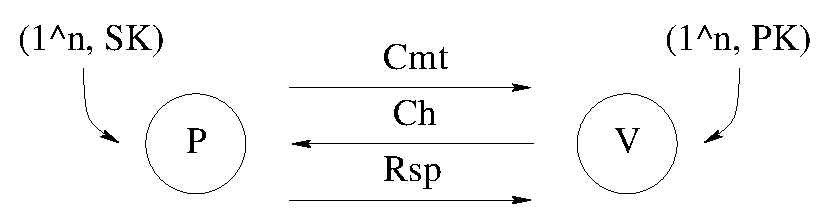
\includegraphics[width = 0.6\textwidth]{../figures/CanonicalIdScheme}
    \caption{The interaction between $P$ and $V$}
    \label{FIG:CanonicalID}
\end{figure}

%When run on input $1^n$, $G$ outputs a pair of keys $(PK,SK)$, where
%$PK$ is the public key and $SK$ is the private key.  
Since the behaviour of $V_{PK}$ is completely determined once his random tape
\textsc{Ch} is fixed, we may think of $V_{PK}$ as a deterministic function
accepting or rejecting ``transcripts'' of the form $(m_1,\textsc{Ch},m_2)$,
where $m_1$ and $m_2$ are the first and second messages received by $V_{PK}$,
respectively; $V_{PK}$ may interact with an adversary who is not $P_{SK}$, so these
need not equal \textsc{Cmt} and \textsc{Rsp}. We require that $P_{SK}$ always
convince $V_{PK}$ to accept, so that
$V_{PK}(\textsc{Cmt},\textsc{Ch},\textsc{Rsp}) = 1$ for all \textsc{Cmt} and
\textsc{Rsp} produced by $P_{SK}$. 

We are interested in two notions of security for identification
schemes: {\it passive security} and {\it active security}.

Informally, $ID$ is {\it passively secure} if no probabilistic polynomial-time
``impersonator'' $I$ who knows $PK$ (but not $SK$)
%given $1^n$ and a public key $PK$ (obtained by
%running $G$ on $1^n$ and some random bits) 
has a 
%non-negligible 
significant probability of convincing $V_{PK}$ to accept when interacting with
him in the role of $P_{SK}$, even after seeing polynomially many transcripts
of conversations between $P_{SK}$ and $V_{PK}$. This weak type of security for
identification schemes is called ``passive'' because $I_{PK}$ passively
monitors the conversation between $P_{SK}$ and $V_{PK}$ without interfering
with it.   

Formally, $I$ is equipped with a ``transcript oracle'' $\fant$. Every time
$\fant$ is queried, it generates a transcript
$(\textsc{Cmt},\textsc{Ch},\textsc{Rsp})$ by running $P_{SK}$ and $V_{PK}$ on
some random bits. $I_{PK}^{\fant}$ is given $1^n$ and a public key $PK$
(generated by running $G$ on $1^n$ and some random bits), together with some
random bits.  $I_{PK}^\fant$ first obtains polynomially many transcripts by
repeatedly querying $\fant$. Next, $I_{PK}^\fant$ sends a commitment
$\textsc{Cmt}'$ to $V_{PK}$, receiving a challenge \textsc{Ch} in reply.
$I_{PK}^\fant$ then responds to the challenge by sending $\textsc{Rsp}'$ to
$V_{PK}$. $ID$ is {\it passively secure} if, for every passive probabilistic
polynomial-time impersonator $I_{PK}^\fant$, the probability $p_I(n)$ that
$V_{PK}(\textsc{Cmt}',\textsc{Ch},\textsc{Rsp}') = 1$ is negligible in $n$;
$p_I(n)$ is taken over the random bits of $G$ (that is, the choice of
$(PK,SK)$), $I_{PK}^\fant$ and $V_{PK}$ (that is, the choice of \textsc{Ch}),
as well as the randomness of $\fant$ (that is, the random bits of $P_{SK}$ and
$V_{PK}$).

Informally, $ID$ is {\it actively secure}, or simply {\it secure}, if no
probabilistic polynomial-time ``impersonator'' $I$ who knows $PK$ (but not
$SK$)
%given $1^n$ and a public key $PK$ (obtained by running $G$ on $1^n$ and some
%random bits) 
has a significant probability of convincing $V_{PK}$ to accept when
interacting with him in the role of $P_{SK}$, even after arbitrarily
interacting with $P_{SK}$ in the role of $V_{PK}$ polynomially many times.
This strong type of security for identification schemes is called ``active''
because $I_{PK}$ actively interacts with $P_{SK}$ rather than merely
monitoring $P_{SK}$'s conversation with $V_{PK}$. 

Formally, we think of $I_{PK}$, who is given $1^n$ and a public key $PK$
(generated by running $G$ on $1^n$ and some random bits), together with some
random bits, as operating in two ``phases''. In the first phase, $I_{PK}$
interacts with $P_{SK}$ (in the role of $V_{PK}$) by sending him polynomially
many adaptively chosen challenges; note that $I_{PK}$ is not constrained to
choose his challenges randomly.
%, but can instead choose them in any way he likes
In the second phase, $I_{PK}$ interacts with $V_{PK}$ (in the role of
$P_{SK}$) as follows. $I_{PK}$ first sends a commitment $\textsc{Cmt}''$ to
$V_{PK}$, receiving a random challenge \textsc{Ch} in reply. $I_{PK}$ then
responds to the challenge by sending $\textsc{Rsp}''$ to $V_{PK}$. $ID$ is
{\it secure} if, for every active probabilistic polynomial-time impersonator
$I_{PK}$, the probability $p_I(n)$ that
$V_{PK}(\textsc{Cmt}'',\textsc{Ch},\textsc{Rsp}'') = 1$ is negligible in $n$;
$p_I(n)$ is taken over the random bits of $G$ (that is, the choice of
$(PK,SK)$), $I_{PK}$, $V_{PK}$ (that is, the choice of \textsc{Ch}) and
$P_{SK}$.

Note that if $V_{PK}$'s challenge $\textsc{Ch}$ is too short,
$|\textsc{Ch}| = \log_2(n)$ say, then the size of the challenge space is only
$2^{|\textsc{Ch}|} = n$. 
%This means that an active impersonator can determine the correct response to
%every possible challenge in polynomial (in fact, linear) time, whereas a
%passive impersonator will receive with non-negligible probability a challenge
%he has already seen the response to. 
An impersonator $I_{PK}$ in possession of even a single valid transcript
$(\textsc{Cmt},\textsc{Ch},\textsc{Rsp})$, obtained through either interacting
with $P_{SK}$ or querying $\fant$, can in this case break the security of $ID$ as
follows. $I_{PK}$ sends \textsc{Cmt} to $V_{PK}$, receives a challenge
$\textsc{Ch}'$ from $V_{PK}$ and sends \textsc{Rsp} to $V_{PK}$ in response. Since $V_{PK}$
accepts whenever $\textsc{Ch}' = \textsc{Ch}$, which happens with probability
$\frac{1}{n}$ (and possibly even if $\textsc{Ch}' \neq \textsc{Ch}$),
$I_{PK}$'s success probability is non-negligible.  In order for $ID$ to hope
to satisfy either of the above two definitions of security, the challenge
space must therefore be of size super-polynomial in $n$, meaning that
$|\textsc{Ch}| = \omega(\log n)$. 

Observe that passive security is strictly weaker than active security, since
every actively secure $ID$ is also passively secure, but not vice versa.
Active security implies passive security because, for every (passive)
impersonator $I_{PK}^\fant$ who breaks the passive security of $ID$, there is
a corresponding (active) impersonator $I_{PK}$ who breaks the active security
of $ID$: $I_{PK}$ simply simulates $I_{PK}^\fant$, taking care to accumulate
enough valid transcripts during the first phase (by choosing the challenges he
sends to $P_{SK}$ randomly) to answer all of $I_{PK}^\fant$'s $\fant$ queries; 
$I_{PK}$'s success probability is identical to that of $I_{PK}^\fant$. 

To see that passive security does {\it not} imply active security, consider
the following (admittedly rather contrived) modification $ID'$ of an arbitrary passively secure
identification scheme $ID$ (such identification schemes exist if one-way
functions do, as we'll see below); we may assume without loss of generality that
$|\textsc{Ch}| = n$. $ID'$ is identical to $ID$, except that whenever the new
prover $P_{SK}'$ receives the challenge $\bar{0} = 0^n$, he responds by
revealing the private key $SK$. $ID'$ remains passively secure, since a
passive impersonator $I_{PK}^\fant$ whose running time is bounded above by
some polynomial $p(\cdot)$ in the security parameter $n$ will see a transcript
containing $SK$ with probability at most $\frac{p(n)}{2^n}$, which is
negligible. However, it is completely trivial for an active impersonator
$I_{PK}$ to break the (active) security of $ID'$: $I_{PK}$ sends $\bar{0}$ to
$P_{SK}'$ to obtain the secret key $SK$ in the first phase, then simulates
$P_{SK}'$ in order to correctly respond to $V_{PK}'$'s challenge in the second phase.

Finally, observe that secure identification schemes exist if and only if
one-way functions do. To see that if secure identification schemes exist then
so do one-way functions, let $ID = (G,P,V)$ be an arbitrary secure canonical
identification scheme. The function $f_{G}$ mapping the random
bits $r$ of $G$ to the public key $PK$ must be one-way, since otherwise an
impersonator could completely break the security of $ID$ (see
Section~\ref{SEC:Signatures}). To see that secure canonical identification
schemes exist if one-way functions do, we need only show how to convert
an arbitrary secure signature scheme into a secure canonical identification
scheme (recall that secure signature schemes exist if one-way functions do). 

We can easily obtain a canonical identification scheme $ID = (G,P,V)$ from any
signature scheme $SIG = (GEN,SIGN,VER)$; $V$ simply challenges $P$ to sign a
random $n$-bit message \textsc{Ch} and accepts only if \textsc{Rsp} is a valid
signature of \textsc{Ch}. Specifically, $G$ is the same as
$GEN$ (so that $(pub,pri) = (PK,SK)$), \textsc{Cmt} = $\lambda$, \textsc{Rsp}
= $SIGN_{SK}(\textsc{Ch})$ and $V_{PK}(\lambda,\textsc{Ch},\textsc{Rsp}) =
VER_{PK}(\textsc{Ch},\textsc{Rsp})$. 

It's not too hard to see that if $SIG$ is secure (as a signature scheme) then
$ID$ is secure (as an identification scheme). An active
impersonator $I$ which successfully breaks the security of $ID$ first gets to
see the signatures of polynomially many messages of his choice and then
successfully signs a random message \textsc{Ch}, whose signature he almost
certainly hasn't already seen (because the challenge space is of
super-polynomial size); a polynomial-time forger $F^\fans$ with access to a
signature oracle $\fans$ can easily simulate $I$, thereby breaking the security
of $SIG$. 
%This means that if one-way functions exist then so do secure
%canonical identification schemes, because secure signature schemes exist if
%one-way functions do.

\section{Public-key encryption schemes}
\label{SEC:PKEPs}
A {\it public-key encryption scheme} $PKE$ consists of three 
polynomial-time algorithms: a key generator $GEN$, an encryptor $ENC$ and a
decryptor $DEC$. $GEN$ and $ENC$ are probabilistic (our definition of security
will crucially depend on the fact that $ENC$ is probabilistic), whereas
$DEC$ is deterministic. 

Informally, the setup is that a person $A$ wants to securely communicate with
some stranger $B$ he knows nothing about, except for his name and address.  To
this end, $A$ generates a pair of keys $(pub,pri)$ using $GEN$, sends the public
key $pub$ to $B$ and keeps the private key $pri$ for himself.  To communicate
a message $m$ to $A$, $B$ obtains an encryption $e_m$ of $m$ using $ENC$ and
sends $e_m$ to $A$; $A$ then decrypts $e_m$ using $DEC$. 
%Security in this
%setting means that no probabilistic polynomial-time adversary $ADV$ who is
%given $pub$ and $e_m$ (but not $pri$) can ``learn'' any information about $m$,
%even after seeing the decryptions of polynomially many messages of his choice.
%
%Observe that communication between $A$ and $B$ as we've defined it is
%unidirectional ($B$ only talks and $A$ only listens), whereas we would like
%$A$ and $B$ to have a normal conversation. One way to accomplish this is for
%$B$ to generate his own pair of keys $(pub',pri')$ using $GEN$ and send $pub'$
%to $A$.  However, that isn't necessary in practice, since $B$ can simply send
%an encryption of a random key $k$ to $A$. Once $A$ and $B$ share a random key,
%they can securely communicate using ``private-key encryption''. In other
%words, public-key encryption schemes can be used for ``secure key exchange''.
%, though the standard notions of security are in some sense ``overkill'' in that case.

For reasons of modularity and efficiency, public-key encryption schemes are in
practice almost always used solely to securely exchange a ``short'' private
key $k$, whose length we'll assume to be equal to the security parameter $n$
for convenience. Once both $A$ and $B$ are in possession of $k$, they can
securely communicate using highly efficient ``private-key encryption''. Thus,
unlike in the case of signature schemes, where we insisted that
$SIGN$ be able to sign messages of arbitrary length, here we will only require
$ENC$ to be able to encrypt $n$-bit messages.  

Formally, $GEN$, $ENC$ and $DEC$ work as follows.

\begin{itemize}

\item Given $1^n$ and some random bits, $GEN$ outputs a pair of keys
$(pub,pri)$, where $pub$ is the public key and $pri$ is the private key.

\item Given $1^n$, $pub$, a message $m \in \strs{n}$ and some random bits,
$ENC$ outputs an encryption $e_m \in \strs{p(n)}$ of $m$, where $p(\cdot)$ is
some polynomial.

\item Given $1^n$, $pri$ and a supposed encryption $\alpha$, $DEC$ either
outputs a message $m \in \strs{n}$ or a special symbol $\bot$ indicating a
failure to decrypt.

\end{itemize}
Denote the output of $ENC$ given $1^n$, $pub$, $m \in \strs{n}$ and some random
bits by $ENC_{pub}(m)$, and the output of $DEC$ given $1^n$, $pri$ and 
$\alpha \in \strs{p(n)}$ by $DEC_{pri}(\alpha)$.  We require that $DEC$
correctly decrypt all encryptions produced by $ENC$, so that for all $n$, all
key pairs $(pub,pri)$ generated by running $GEN$ on $1^n$ and some random bits,
all messages $m \in \strs{n}$ and all encryptions $e_m = ENC_{pub}(m)$,
$DEC_{pri}(e_m) = m$. 

We are interested in two notions of security for public-key encryption
schemes: {\it semantic security} and {\it chosen-ciphertext security}.

Informally, $PKE$ is {\it semantically secure} (\cite{goldwasser:probenc2}) if
no probabilistic polynomial-time ``eavesdropper'' $E$ who knows $pub$ (but not
$pri$) and passively monitors the channel between $A$ and $B$ can ``learn''
even a single bit of information about a message $m$ through seeing its
encryption $e_m$. 

Formally, $E$ is given $1^n$ and a public key $pub$ (generated by running
$GEN$ on $1^n$ and some random bits) and chooses two distinct $n$-bit
messages, $m_0$ and $m_1$. A bit $b$ is then chosen randomly (but not shown to
$E$), and $E$ is given an encryption $e_b = ENC_{pub}(m_b)$ of $m_b$. $E$ next
computes for a while, finally outputting a bit $b'$. Let $p_{E}(n)$ be the
probability that $b' = b$, meaning that $E$ correctly determined $b$;
$p_{E}(n)$ is taken over the random bits of $E$ and $GEN$ (that is, the choice
of $(pub,pri)$), as well as the choice of $b$.  $PKE$ is {\it semantically
secure} if, for every probabilistic polynomial-time eavesdropper $E$,
$|\frac{1}{2} - p_{E}(n)|$ is negligible in $n$ (in other words, $p_{E}(n)$
doesn't significantly differ from $\frac{1}{2}$, the probability of randomly
guessing $b$).

Note that $PKE$ cannot be semantically secure if $ENC$ is deterministic. In
order to break the semantic security of $PKE$, an eavesdropper
$E$ (who knows $pub$) simply computes $\eta_0 = ENC_{pub}(\bar{0})$ and
$\eta_1 = ENC_{pub}(\bar{1})$, where $\bar{0} = 0^n$ and $\bar{1} = 0^{n-1}1$,
then sets $m_0 = \bar{0}$ and $m_1 = \bar{1}$.  Once $E$ receives $e_b$, he
outputs 0 if $e_b = \eta_0$ and 1 if $e_b = \eta_1$ (these are the only two
possibilities because $ENC$ is deterministic). Since $E$ always outputs $b$
correctly (so that $b' = b$ with probability 1), $|\frac{1}{2} - p_E(n)| =
\frac{1}{2}$, which is certainly non-negligible.
 
Informally, $PKE$ is {\it secure against (adaptive) chosen-ciphertext attack}
or {\it CCA2-secure} (\cite{rackoff:cca2}) if no probabilistic polynomial-time
adversary $ADV$ who knows $pub$ (but not $pri$) and has complete control over
the channel between $A$ and $B$ can ``learn'' even a single bit of information
about a message $m$ through seeing its encryption $e_m$. What does it mean for
$ADV$ to have ``complete control'' over the channel between $A$ and $B$?
Intuitively, $ADV$ intercepts all encryptions or ``ciphertexts'' sent by $A$
to $B$ and sends $B$ whatever he likes instead.

Formally, $ADV$ is given $1^n$ and a public key $pub$ (generated by running
$GEN$ on $1^n$ and some random bits) and equipped with a ``decryption oracle''
$\fand$, which outputs $DEC_{pri}(\alpha)$ when queried on a ciphertext
$\alpha \in \strs{p(n)}$.  $\fand$ is meant to capture the intuition that
$ADV$ can effectively force $B$ to decrypt any ciphertext of his choosing (of
course the answer may well be $\bot$; we think of ``ciphertexts'' that decrypt
to $\bot$ as being malformed).

$ADV^\fand$ queries $\fand$ on $\alpha_0$ and receives $DEC_{pri}(\alpha_0)$,
queries $\fand$ on $\alpha_1$ and receives $DEC_{pri}(\alpha_1)$, and so on.
Since $ADV^\fand$ may in general choose his queries based on $\fand$'s
previous answers, this is an adaptive attack.  Eventually, $ADV^\fand$ chooses
two distinct $n$-bit messages, $m_0$ and $m_1$. A bit $b$ is then chosen
randomly (but not shown to $ADV^\fand$), and $ADV^\fand$ is given an
encryption $e_b = ENC_{pub}(m_b)$ of $m_b$. 

$ADV^\fand$ now gets to query $\fand$ on some additional ciphertexts, whose
choice may in general depend on $e_b$.  Naturally, we don't allow $ADV^\fand$
to query $\fand$ on $e_b$ itself, since $DEC_{pri}(e_b)$ uniquely determines
$b$ (because $m_0 \neq m_1$). Alternatively, once $ADV^\fand$ receives $e_b$
we could forbid him from querying $\fand$ altogether; security against this
type of ``lunchtime attack'' is called {\it CCA1 security} (\cite{naor:cca1}).
However, that would arguably be too restrictive, since in practice CCA2
security is almost always broken by querying $\fand$ on ciphertexts ``related
to'' (though not the same as) $e_b$.

$ADV^\fand$ next computes for a while, finally outputting a bit $b'$.  Let
$p_{ADV}(n)$ be the probability that $b' = b$, meaning that $ADV^\fand$
correctly determined $b$; $p_{ADV}(n)$ is taken over the random bits of
$ADV^\fand$ and $GEN$ (that is, the choice of $(pub,pri)$), as well as the
choice of $b$ (the decryption oracle $\fand$ is deterministic).
$PKE$ is {\it CCA2 secure} if, for every probabilistic polynomial-time
adversary $ADV^\fand$, $|\frac{1}{2} - p_{ADV}(n)|$ is negligible in $n$ (in
other words, $p_{ADV}(n)$ doesn't significantly differ from $\frac{1}{2}$, the
probability of randomly guessing $b$).

Observe that semantic security is strictly weaker than CCA2 security, since
every CCA2-secure $PKE$ is also semantically secure, but not vice versa. CCA2
security implies semantic security because, for every eavesdropper $E$ who
breaks the semantic security of $PKE$, there is a corresponding adversary
$ADV^\fand$ who breaks the CCA2 security of $PKE$: $ADV^\fand$ simply
simulates $E$, ignoring the decryption oracle $\fand$; $ADV^\fand$'s success
probability is identical to that of $E$. This implies that $PKE$ cannot be
CCA2-secure if $ENC$ is deterministic --- we already know that such a $PKE$ is
not semantically secure, and we just showed every CCA2-secure public-key
encryption scheme is.

To see that semantic security does {\it not} imply CCA2 security, consider the
following (admittedly rather contrived) modification $PKE'$ of an arbitrary
semantically secure public-key encryption scheme $PKE$. $PKE'$ is identical to
$PKE$, except that the new encryptor $ENC'$ appends an additional bit, say 0
for concreteness, to every encryption; this bit is ignored by the new
decryptor $DEC'$. $PKE'$ remains semantically secure, since, for every
eavesdropper $E'$ who breaks the semantic security of $PKE'$, there is a
corresponding eavesdropper $E$ who breaks the semantic security of $PKE$: $E$
simulates $E'$ to obtain a pair of messages $(m_0,m_1)$, receives
an encryption $e_b$ and gives $e_b 0$ to $E'$, accepting if and only if $E'$
accepts; $E$'s success probability is identical to that of $E'$. 

However, it is completely trivial for an adversary $ADV^\fand$ to break the
CCA2 security of $PKE'$: $ADV^\fand$ sets $m_0 = \bar{0}$ and $m_1 = \bar{1}$,
receives $e_b = ENC'_{pub}(m_b)$, and queries $\fand$ on $e_b 1$ to obtain a
decryption $m'$. He then outputs $0$ if $m' = \bar{0}$ and $1$ if $m' =
\bar{1}$ (these are the only two possibilities, since $DEC'$ ignores the
trailing bit). Since $ADV^\fand$ always outputs $b$ correctly (so that $b' =
b$ with probability 1), $|1 - p_{ADV}(n)| = \frac{1}{2}$, which is certainly
non-negligible.  Although our highly artificial modification of $PKE$ may seem
like a cheat, in practice public-key encryption schemes fail to be CCA2-secure
for the same reason as $PKE'$. Namely, they are ``malleable'', which
informally means that an adversary $ADV^\fand$ can ``malleate'' (that is,
modify) $e_b$ into some related encryption $e'_b$ such that $b$ can be
computed from $\fand(e'_b)$ ($ADV^\fand$ is allowed to query $\fand$ on $e_b'$
since $e_b' \neq e_b$).

\section{The Random Oracle Model (ROM)}
\label{SEC:ROM}
The Random Oracle Model, or ROM for short, is a setting where all parties have
access to a ``random oracle'' $\fanr$. The ROM was formally introduced
in the context of cryptography in \cite{bellare:rompractical}. 

One way to think of $\fanr$ is as a randomly chosen function mapping
$\strs{*}$ to $\strs{n}$\symbolfootnote[2]{In general, $\fanr$ maps $\strs{*}$
to $\strs{\ell(n)}$, where $\ell(n) \leq n^c$ for some $c$. However, we will
usually assume that $\ell(n) \equiv n$ to simplify the presentation.}.
%, where $p(\cdot)$ is some polynomial in the security
%parameter $n$ (for convenience, we often assume that
%assume without loss of generality
%$p(n) \equiv n$). 
However, the set of all such functions is (countably)
infinite, and we prefer not to talk about sampling such sets.
%it doesn't formally make sense to talk about sampling infinite sets in this
%case. 
Instead, we view $\fanr$ as choosing his answers ``on-line''.  When
queried on $q \in \strs{*}$, $\fanr$ first checks whether $q$ is a ``new
query'', meaning that he hasn't been queried on $q$ before. If so, he randomly
chooses a response $ans \in \strs{n}$ to $q$, writes $ans$ down somewhere
and then outputs it.  Otherwise (namely in the case that $\fanr$ has been
queried on $q$ already), he looks up and outputs his previous response to $q$;
this ensures that identical queries receive an identical response (which is
the case when $\fanr$ is viewed as a function).  
%Although in this way $\fanr$'s responses are not ``filled-in'' until the
%corresponding queries are asked, the resulting distribution over responses
%agrees with our intuition about randomly choosing $\fanr$ from among all
%functions mapping $\strs{*}$ to $\strs{p(n)}$.

We next show that, in some appropriate sense at least, random oracles are
one-way (see Section~\ref{SEC:Oneway} for a definition of one-wayness).  Let
$p_{INV}(n)$ denote the probability that a probabilistic polynomial-time
inverter $INV^\fanr$ who 
%has oracle access to $\fanr$ and 
is given $y = \fanr(x) \in \strs{n}$ for a randomly chosen $x \in \strs{n}$
outputs an $x' \in \strs{n}$ such that $\fanr(x') = y$; $p_{INV}(n)$ is taken
over the choice of $x$, the random bits of $INV^\fanr$ and the randomness of
$\fanr$. Observe that $y$ yields no information about $x$, since it is
distributed uniformly over $\strs{n}$ no matter what $x$ is. Denote the
strings $INV^\fanr$ queries $\fanr$ on by $x_1,\ldots,x_{q_\fanr}$, and set
$y_i = \fanr(x_i)$ for $1 \leq i \leq q_\fanr$;
%$INV^\fanr$'s best strategy is therefore to choose as many distinct strings
%$x_i \in \strs{n}$ as possible, query $\fanr$ on each $x_i$ to obtain $y_i =
%\fanr(x_i)$, and hope that there exists an $i$ such that $y_i = y$.  Denote
%the number of times $INV^\fanr$ queries $\fanr$ by $q_\fanr$, 
notice that $q_\fanr \leq n^c$ for some $c$,
because $INV^\fanr$ runs in (strict) polynomial time. $INV^\fanr$ wins if
there is an $1 \leq i \leq q_\fanr$ such that either $x_i = x$ or $x_i \neq x$
but $y_i = y$ anyway. Applying the union bound, we see that this happens with probability at most
$\frac{2q_\fanr}{2^n} \leq \frac{2n^c}{2^n}$, which is negligible.
%For every $1 \leq j \leq
%q_\fanr$, we have:
%\begin{align*}
%\text{Pr}[y_j = y] &= \text{Pr}[y_j = y \mid x_j = x]\cdot\text{Pr}[x_j = x] 
%+ \text{Pr}[y_j = y \mid x_j \neq x]\cdot\text{Pr}[x_j \neq x] \\ &=
%\frac{1}{2^n - (j-1)} + \frac{1}{2^n}\left(1 - \frac{1}{2^n - (j-1)}\right)
%\leq \frac{1}{2^n - (j-1)} + \frac{1}{2^n} \\ &\leq \frac{2}{2^n - j + 1}
%\leq \frac{2}{2^n - q_\fanr + 1} \end{align*} Applying the union bound then
%gives $p_{INV}(n) \leq \frac{2q_\fanr}{2^n - q_\fanr + 1} \leq
%\frac{2n^c}{2^n - n^c + 1}$, which is negligible in $n$.  \[ \text{Pr}[x = x'
%\mid y = y'] = \frac{1}{2^{p(n)}} \text{ for all } x' \in \strs{n} \text{ and
%}y' \in \strs{p(n)},
%\]
%so that $y$ yields no information about $x$ (here the probability is taken
%over the choice of $x$ and the randomness of $\fanr$). 
%This means that $p_{INV}(n) \leq
%\frac{q_\fanr}{2^{p(n)}} \leq \frac{n^c}{2^{p(n)}}$, which is negligible in
%$n$.


\chapter{On the security of Fiat-Shamir signature schemes in the ROM}
\label{CH:Fiatshamir}

\section{Fiat-Shamir signature schemes: an overview} 
\label{SEC:Overview}
In their seminal 1986 paper (\cite{fiat:fsparadigm}), Amos Fiat and Adi Shamir
proposed a new, highly efficient signature scheme based on a certain canonical
identification scheme closely related to the protocols presented in
\cite{goldwasser:ips1} and \cite{fischer:obtransfer} (for definitions of
signature schemes and canonical identification schemes, see
Sections~\ref{SEC:Signatures} and \ref{SEC:IDschemes} of
Chapter~\ref{CH:Preliminaries}). Such signature schemes are now called
``Fiat-Shamir signature schemes'', whereas Fiat and Shamir's approach itself
is referred to as the ``Fiat-Shamir paradigm''. Essentially, their idea was as
follows.
%to eliminate the
%verifier's random move using a ``cryptographic hash function'' $h$. 
In order to sign a message $m$, simply simulate the prover, replacing the
verifier's random challenge with $h(m)$, where $h$ is some ``cryptographic
hash function'' (actually, this isn't quite right, as we'll see below). The
resulting transcript then serves as a signature of $m$.
%enabling valid transcripts to serve as signatures.  To sign a message $m$,
%one first obtains a commitment \textsc{Cmt} by simulating the prover, then
%computes a challenge $\textsc{Ch}_m = h(\textsc{Cmt},m)$ (here and below ','
%doubles as the string concatenation operator), and finally obtains a response
%\textsc{Rsp} by simulating the prover (who is assumed to ``remember''
%\textsc{Cmt}) on $\textsc{Ch}_m$. The transcript $(\textsc{Ch},\textsc{Rsp})$
%is then used a signature of $m$.

Fiat and Shamir showed that the signature scheme in question is secure if $h$
is ``truly random'', provided that taking square roots modulo $N = pq$, where
$p$ and $q$ are unknown ``large'' primes, is hard (a standard hardness
assumption). In modern terminology, Fiat and Shamir effectively showed that
the signature scheme is secure in the Random Oracle Model, or ROM (see
Chapter~\ref{CH:Preliminaries}, Section~\ref{SEC:ROM} for a discussion of the
ROM), under a standard hardness assumption. Although this may strike one as a
rather weak security guarantee, no practical signature schemes provably secure
under standard hardness assumptions were known at the time.  Today, a number
of highly efficient signature schemes provably secure under such
``non-standard-yet-plausible'' hardness assumptions as the ``strong RSA
assumption'' and the ``strong Computational Diffie-Hellman assumption'' are
available (\cite{gennaro:fastsigs}, \cite{cramer:signatures2},
\cite{fischlin:cramershoup}, \cite{boneh:shortsigsnorom}). 

Various other Fiat-Shamir signature schemes which are provably secure in the
ROM under standard hardness assumptions have been described over the years
(\cite{micali:betterfs}, \cite{okamoto:discretelogfs}, \cite{shoup:practid},
\cite{goh:romcdh}), but until fairly recently it was not known whether {\it
every} (actively) secure canonical identification scheme yields a Fiat-Shamir
signature scheme secure in the ROM. While Abdalla et al. showed in
\cite{abdalla:fiatshamirrom} that secure ``non-trivial'' canonical
identification schemes yield Fiat-Shamir signature schemes secure in the ROM
(informally, a canonical identification scheme is ``non-trivial'' if the
prover's commitment distribution has ``high entropy''), they left open the
question of whether secure ``trivial'' canonical identification schemes do. In
Section~\ref{SEC:OurResult}, we prove that every secure canonical
identification scheme, trivial or not, does indeed yield a Fiat-Shamir
signature scheme secure in the ROM.

However, as we will see in Chapter~\ref{CH:Uninstantiability}, security in the
ROM is no guarantee of real-world security. In
\cite{goldwasser:fsparadigmfails}, Goldwasser and Tauman show that there exist
Fiat-Shamir signature schemes which, although secure in the ROM, are
``uninstantiable'' (see Chapter~\ref{CH:Uninstantiability},
Section~\ref{SEC:FiatShamir}). Such schemes are not secure in the ``real
world'', no matter what hash function ensemble is used to ``instantiate'' the
random oracle.
%
%Given a canonical identification scheme $ID$ and a ``cryptographic hash
%function'' $h$ (or, more properly, an ensemble $\{\fanh_n\}_{n \in \nats}$ of
%such functions), denote the resulting Fiat-Shamir signature scheme by
%$SIG_h(ID)$. A fundamental question is whether, for every (actively) secure
%$ID$, there exists an $h$ such that $SIG_h(ID)$ is secure in the ``real
%world'' (as opposed to merely in the ROM). Building on the pioneering work of
%Canetti, Goldreich and Halevi (\cite{canetti:romfails}), Goldwasser and
%Tauman gave a negative answer in \cite{goldwasser:fsparadigmfails}. Although
%Goldwasser and Tauman's result does not imply that any of the Fiat-Shamir
%signature schemes actually used in practice are insecure, it fatally
%undermines the validity of the ``Fiat-Shamir paradigm''.

\section{The Fiat-Shamir transform}
\label{SEC:FiatShamirTransform}
Let $ID = (G,P,V)$ be a canonical identification scheme and $h$ be a
``cryptographic hash function''. The function mapping $ID$ and $h$ to the
corresponding Fiat-Shamir signature scheme $SIG_h(ID)$ is sometimes called the
``Fiat-Shamir transform''. Since this thesis is primarily concerned with
security in the ROM, 
%here 
we will only present the transform's ROM version,
which maps $ID$ to $SIG(ID) = (G,SIGN^\fanr,VER^\fanr)$.

Given $1^n$, a private key $SK$ (generated by running $G$ on $1^n$ together
with some random bits), a message $m \in \strs{*}$ and some random bits, the
signer $SIGN^\fanr$ proceeds as follows. He first simulates $P_{SK}$ to obtain
a commitment \textsc{Cmt} and computes a challenge $\textsc{Ch}_m =
\fanr(\textsc{Cmt}, m)$ by querying $\fanr$;
note that the challenge depends on the message to be signed.  $SIGN^\fanr$
then simulates $P_{SK}$ on $\textsc{Ch}_m$ to obtain a response $\textsc{Rsp}$
and outputs $\sigma_m = (\textsc{Cmt},\textsc{Rsp})$ as the signature of $m$.
(Recall that $P_{SK}$ denotes the behaviour of $P$ when given $1^n$, $SK$ and
some random bits $r$. Specifically, $P$ computes a commitment
\textsc{Cmt} as a function of $1^n$, $SK$ and $r$, receives a challenge
\textsc{Ch}, and then computes a response \textsc{Rsp} as a function of $1^n$,
$SK$, $r$ and \textsc{Ch}).

Given $1^n$, a public key $PK$ (generated by running $G$ on $1^n$ together
with some random bits), a message $m \in \strs{*}$ and a supposed signature
$(\alpha,\gamma)$ of $m$, the verifier $VER^\fanr$ simply computes $\beta =
\fanr(\alpha,m)$ by querying $\fanr$ and outputs
$V_{PK}(\alpha,\beta,\gamma)$ (Recall that $V_{PK}$ is a deterministic
function of $(\alpha,\beta,\gamma)$).

Our goal is to show that if $ID$ is secure then $SIG(ID)$ is secure in the
ROM. By security in this setting we mean the ordinary security for signature
schemes (that is, security against existential forgery under adaptive
chosen-message attack), except that the forger $F$ now has access to
the random oracle $\fanr$ in addition to the signature oracle $\fans$, and
his success probability is also taken over the randomness of $\fanr$.

\section{An earlier result}
\label{SEC:OldResult}
Abdalla, An, Bellare and Namprempre present several results concerning the
Fiat-Shamir transform in \cite{abdalla:fiatshamirrom}, including a randomized
version of the transform and applications to ``forward-secure signature
schemes''. However, we are only interested in the following result of theirs:
%the only result of interest to us is the following: 
for every passively secure ``non-trivial'' canonical identification scheme
$ID$, the corresponding Fiat-Shamir signature scheme $SIG(ID)$ is secure in
the ROM. Since active security implies passive security for identification
schemes, this means that every secure ``non-trivial'' canonical identification
scheme yields a Fiat-Shamir signature scheme secure in the ROM. 

Informally, $ID$ is ``non-trivial'' if the prover's commitment distribution
has ``high entropy''. Formally, let $\fanp_{SK} = \{p_i\}_{i=0}^k$ denote
$P_{SK}$'s commitment distribution and define the {\it min-entropy} of
$\fanp_{SK}$ by $H_{\min}(\fanp_{SK}) = -\log_2(p_{\max})$, where
$p_{\max} = \max\{p_i\}_{i=0}^k$ is the largest probability mass in
$\fanp_{SK}$.  $ID$ is {\it non-trivial} if $\min\{H_{\min}(\fanp_{SK}) : SK
\gets G(1^n)\} = \omega(\log n)$, meaning that the minimum min-entropy of
$\fanp_{SK}$, taken over all private keys $SK$ (generated by running $G$ on
$1^n$ and some random bits), is super-logarithmic in the security parameter
$n$. It can be shown that in this case the probability of seeing the same
commitment more than once in polynomially many trials is negligible, so that,
for all practical purposes, $P_{SK}$'s commitments don't repeat. Canonical
identification schemes which are not non-trivial are said to be {\it trivial}.

Let $ID$ be a non-trivial canonical identification scheme. Suppose that
$F^{\fanr,\fans}$ is a polynomial-time forger who breaks the security of
$SIG(ID)$ in the ROM, and denote his (non-negligible) success probability by
$p_F(n)$.  $F^{\fanr,\fans}_{PK}$ is given $1^n$, $PK$ and some random bits,
and his goal is to output a new message $m^*$ (i.e. one he hasn't
queried $\fans$ on) together with a valid signature $\sigma^* =
(\textsc{Cmt}^*,\textsc{Rsp}^*)$ of $m^*$.

We may assume, without loss of generality, that $F^{\fanr,\fans}_{PK}$ doesn't
query $\fanr$ on any string more than once, since that would yield no new
information (because $\fanr$'s responses would all be identical).  We may
additionally assume, again wlog, that $F^{\fanr,\fans}_{PK}$ doesn't query
$\fanr$ on strings whose length is less than $\ell(n)$; recall that all of
$P_{SK}$'s commitments are of length $\ell(n)$.  $\fanr$ queries involving
such ``short strings'' can safely be answered randomly, since there is no
interplay between them and $\fans$ queries (more on this interplay later).
This assumption ensures that every $s \in \strs{*}$ $F^{\fanr,\fans}_{PK}$
queries $\fanr$ on can be parsed as $(\textsc{Cmt},m)$, where $\textsc{Cmt}
\in \strs{\ell(n)}$ and $m \in \strs{*}$.  Finally, it will be convenient for
us to assume that $F^{\fanr,\fans}_{PK}$ queries $\fanr$ on
$(\textsc{Cmt}^*,m^*)$ at some point during his execution; following the
terminology of \cite{abdalla:fiatshamirrom}, we refer to this special $\fanr$
query as the ``crucial query''. There is no loss of generality in assuming
that the forger makes the crucial query, since every $F^{\fanr,\fans}$ who
doesn't can easily be converted into a corresponding forger
$\hat{F}^{\fanr,\fans}$ who does: $\hat{F}^{\fanr,\fans}_{PK}$ obtains $m^*$
and $\sigma^* = (\textsc{Cmt}^*,\textsc{Rsp}^*)$ by simulating
$F^{\fanr,\fans}_{PK}$, queries $\fanr$ on $(\textsc{Cmt}^*,m^*)$ and then
outputs $(m^*,\sigma^*)$.  Since the additional $\fanr$ query doesn't affect
the choice of $m^*$ and $\sigma^*$, $\hat{F}^{\fanr,\fans}$'s success
probability is identical to that of $F^{\fanr,\fans}$.
%Observe that the
%total number of queries asked by $F^{\fanr,\fans}$, and in particular the
%number of his $\fanr$ queries, is bounded above by $n^c$ for some $c$ (where
%$n$ is the security parameter), since $F^{\fanr,\fans}$ runs in (strict)
%polynomial time.  
%
%Let $q_\fanr(n)$ denote the number of times $F^{\fanr,\fans}$ queries $\fanr$,
%and consider the following passive impersonator $I^\fant$. Given $1^n$, $PK$
%and some random bits, $I^\fant$ first guesses the index of $F^{\fanr,\fans}$'s
%crucial query by randomly choosing $i \in \{1,\ldots,q_\fanr(n)\}$, and then
%simulates $F^{\fanr, \fans}$ on $1^n$ and $PK$, answering all of his $\fanr$
%queries but the $i^{th}$ randomly (the $i^{th}$ query is treated specially)
%and his $\fans$ queries using $\fant$. Specifically, $I^\fant$ responds to all
%
%Whenever $F^{\fanr,\fans}$ queries $\fanr$ on some string $q$, $I^\fant$
%randomly chooses a response $ans \in \strs{n}$ and gives it to
%$F^{\fanr,\fans}$ (recall that $F^{\fanr,\fans}$ doesn't query $\fanr$ on the
%same string more than once, by assumption). Whenever $F^{\fanr,\fans}$
%queries $\fans$ on some message $m \in \strs{*}$, $I^\fant$ obtains a new
%transcript $(\textsc{Cmt},\textsc{Ch},\textsc{Rsp})$ from $\fant$ and gives
%$(\textsc{Cmt},\textsc{Rsp})$ to $F^{\fanr,\fans}$ as the signature of $m$.
%
%Denote $I^\fant$'s success probability (i.e. the probability that he breaks the
%security of $ID$) by $p_I(n)$, and $F^{\fanr,\fans}$'s success probability
%(i.e. the probability that he breaks the security of $SIG(ID)$) by
%$p_F(n)$. We'll see below that, although $p_I(n)$ is not identical to
%$p_F(n)$, the difference between the two is negligible. Since $p_F(n)$ is
%non-negligible by assumption, this means that $p_I(n)$ is also non-negligible,
%so that $I^\fant$ breaks the security of $ID$. 
%
%Recall that signing in $SIG(ID)$ is probabilistic, so it makes sense for
%$F^{\fanr,\fans}$ to ask to see multiple signatures of the same message $m$.
%Suppose that $F^{\fanr,\fans}$ queries  $\fans$ on $m$ twice, and $I^\fant$
%responds to the first query using the transcript $T_1 =
%(\textsc{Cmt},\textsc{Ch},\textsc{Rsp})$ and to the second using $T_2 =
%(\textsc{Cmt}',\textsc{Ch}',\textsc{Rsp}')$. Since $T_1$ and $T_2$ are valid
%transcripts, we have $V_{PK}(\textsc{Cmt},\textsc{Ch},\textsc{Rsp}) = 1$ and
%$V_{PK}(\textsc{Cmt}',\textsc{Ch}',\textsc{Rsp}') = 1$. In order for both
%$\sigma_1 = (\textsc{Cmt},\textsc{Rsp})$ and $\sigma_2 =
%(\textsc{Cmt}',\textsc{Rsp}')$ to be legitimate signatures of $m$, 
%
%$ID$ is {\bf passively secure} and {\bf nontrivial} $\Rightarrow SIG(ID)$ is
%{\bf secure in the ROM}
%
%\textsc{Proof Sketch}: The proof is by a standard black-box reducibility 
%argument. We show how to convert a forger $F$ which breaks the security of
%$SIG(ID)$ in the ROM into an impersonator $I$ which breaks the passive
%security of $ID$.
%Suppose that we are given a probabilistic polytime forger $F$ which breaks the
%security of $SIG(ID)$ in the ROM. $F$ is given the public key $pub$ and has 
%access to both a random oracle $\fanr$ and a signing oracle $\fans$: every time 
%$\fans$ is queried on a message $m' \in \strs{*}$, it outputs a signature 
%$\sigma' = (\textsc{Cmt}',\textsc{Rsp}')$ of $m'$ such that 
%$V_{pub}(\textsc{Cmt}',\textsc{Ch}',\textsc{Rsp}') = 1$, where 
%$\textsc{Ch}' = \fanr(\textsc{Cmt}',m')$. 
%The probability that $F_{pub}^{\fanr,\fans}$ eventually outputs a new message 
%$m$ together with a signature $\sigma = (\textsc{Cmt},\textsc{Rsp})$ 
%such that $V_{pub}(\textsc{Cmt},\textsc{Ch},\textsc{Rsp}) = 1$, where 
%$\textsc{Ch} = \fanr(\textsc{Cmt},m)$, taken over $(pub,pri) \gets G(1^n)$, 
%the randomness of $\fanr$ and $\fans$ and the coins of $F_{pub}^{\fanr,\fans}$,
%is non-negligible in $n$. 
%Notice that signing in $SIG(ID)$ is probabilistic, so it makes sense for
%$F^{\fanr,\fans}_{pub}$ to query $\fans$ on the same string multiple times. 
%On the other hand, there's nothing to gain from querying $\fanr$ on the same
%string more than once, so we may assume (wlog) that $F^{\fanr,\fans}_{pub}$ 
%does no such thing. 
%We can also safely assume that $F_{pub}^{\fanr,\fans}$ queries $\fanr$ on
%$(\textsc{Cmt},m)$ before outputting $m$ and $\sigma$. If it doesn't, we can
%easily construct another forger, $F_{pub}^{'\fanr,\fans}$, that does: 
%$F_{pub}^{'\fanr,\fans}$ simply simulates $F_{pub}^{\fanr,\fans}$ until the 
%latter outputs a message $m$ and a signature $\sigma)$, then queries $\fanr$ on 
%$(\textsc{Cmt},m)$ and outputs $(m,\sigma)$. This additional random oracle 
%query, which we'll call the ``crucial query'', has no effect on 
%$F_{pub}^{'\fanr,\fans}$'s success probability, since it does not affect the 
%choice of $m$ or $\sigma$. 

We now describe a polynomial-time impersonator $I^\fant$ who, given $1^n$,
$PK$ and some random bits, breaks the passive security of $ID$ (in the real
world) by simulating $F^{\fanr,\fans}_{PK}$.
%key $pub$ and access to a transcript-generating oracle $\fant$, gets
%$V_{pub}$ to accept with probability non-negligible in the security parameter
%$n$. Here the probability is taken over $(pub,pri) \gets G(1^n)$, the
%randomness of $\fant$ and the coins of $I_{pub}^\fant$.  Say that the running
%time of $F_{pub}^{\fanr,\fans}$ is bounded above by $n^c$, no matter what the
%outcome of its coin tosses is; such a $c$ exists since
%$F_{pub}^{\fanr,\fans}$ is assumed to run in strict polynomial time. This
%means that for any random tape, $F_{pub}^{\fanr,\fans}$ makes at most $n^c$
%random oracle queries, which we'll number from 1 to $n^c$. 
Let $q_\fanr(n)$ denote the number of times $F^{\fanr,\fans}_{PK}$ queries
$\fanr$. Since $F^{\fanr,\fans}_{PK}$ runs in (strict) polynomial time,
$q_\fanr(n) \leq n^c$ for some $c$ (in the worst case, $F^{\fanr,\fans}_{PK}$
does nothing but query $\fanr$, each query taking a single step).

$I_{PK}^{\fant}$ begins 
%his simulation of $F_{PK}^{\fanr,\fans}$ 
by 
%guessing the index of the ``crucial query'': he 
randomly choosing an index $i \in \{1,\ldots,q_\fanr(n)\}$; as we'll see later,
$i$ is not revealed to $F^{\fanr,\fans}_{PK}$ in the course of the simulation.  
%and hopes that $F_{PK}^{\fanr,\fans}$'s $i^{th}$ random oracle query is about
%$(\textsc{Cmt}^*,m^*)$. 
Since we've assumed both that $F_{PK}^{\fanr,\fans}$ makes the crucial query
and that he never queries $\fanr$ on the same string more than once, $i$ is
the index of the crucial query with probability $\frac{1}{q_\fanr(n)} \geq
\frac{1}{n^c}$. A technical but important point is that the distribution of
$F^{\fanr,\fans}$'s views (namely what he ``sees'' during the simulation,
including his random bits and the answers to his oracle queries) is
independent of the choice of $i$, so that he gets no information about $i$. If
that were not the case, $F^{\fanr,\fans}_{PK}$ could exploit his knowledge of
$i$ to ensure that $I^\fant_{PK}$ never guesses the index of the crucial query
correctly.
%What does $I_{PK}^\fant$ gain by
%correctly guessing the index of the crucial query? It enables him to parse
%$F^{\fanr,\fans}_{PK}$'s $i^{th}$ $\fanr$ query as $(\textsc{Cmt}^*,m^*)$
%(recall that we're assuming commitments have a fixed length of $\ell(n)$),
%thereby learning the value of $\textsc{Cmt}^*$. The latter can then be sent to
%$V$ to obtain a challenge $\textsc{Ch}$, which can in turn be given to
%$F_{PK}^{\fanr,\fans}$ as the answer to the crucial query. This ensures that 
%$\textsc{Rsp}^*$ is a correct answer to \textsc{Ch}, so that
%$(\textsc{Cmt}^*,\textsc{Ch},\textsc{Rsp}^*)$ is a valid transcript.

During the simulation, $I_{PK}^\fant$ responds to all of
$F_{PK}^{\fanr,\fans}$'s random oracle queries but the $i^{th}$ with a
randomly chosen $n$-bit string (since $F_{PK}^{\fanr,\fans}$ never queries
$\fanr$ on the same string more than once, there is no risk of giving
inconsistent answers). The $i^{th}$ query is handled as follows.  Suppose
that, for his $i^{th}$ random oracle query, $F_{PK}^{\fanr,\fans}$ queries
$\fanr$ on some $s \in \strs{*}$ (recall that $|s| \geq \ell(n)$, since
$F^{\fanr,\fans}_{PK}$ doesn't query $\fanr$ on ``short strings'').
$I_{PK}^{\fant}$ parses $s$ as $(\textsc{Cmt}^*,m^*)$, sends $\textsc{Cmt}^*
\in \strs{\ell(n)}$ to $V_{PK}$, and receives a challenge $\textsc{Ch}^* \in
\strs{n}$ in reply.
%; if $|s| < \ell(n)$ then $I_{PK}^\fant$ sets $m^*$
%to $\lambda$ and pads $s$ with an appropriate number of zeros to obtain a valid
%commitment $\textsc{Cmt}^*$ 
He then gives $\textsc{Ch}^*$ to $F_{PK}^{\fanr,\fans}$ as the answer to
$\fanr(s)$ and continues his simulation. This ensures that $\textsc{Rsp}^*$ is
a correct answer to $\textsc{Ch}^*$, so that
$(\textsc{Cmt}^*,\textsc{Ch}^*,\textsc{Rsp}^*)$ is a valid transcript.

Whenever $F_{PK}^{\fanr,\fans}$ asks to see a signature of a message $m$,
$I_{PK}^\fant$ queries $\fant$ to obtain a valid transcript
$(\textsc{Cmt},\textsc{Ch},\textsc{Rsp})$ and gives
$(\textsc{Cmt},\textsc{Rsp})$ to $F_{PK}^{\fanr,\fans}$. To ensure that future
$\fanr$ queries are answered consistently, $I^\fant$ then sets
$\fanr(\textsc{Cmt},m)$ to \textsc{Ch}.
%There is a problem with this approach if $F_{pub}^{\fanr,\fans}$ queries
%$\fans$ on the same message $m'$ many times, which is a reasonable thing to
%do because signing in $SIG(ID)$ is probabilistic. In order for the resulting
%transcripts to be legitimate signatures of $m'$, it must be the case that
%$\fanr(\textsc{Cmt}',m') = \textsc{Ch}'$ for all of them. $\fant$, however,
%generates $\textsc{Ch}'$ randomly.  If the commitments $\textsc{Cmt}'$ are
%distinct then $\textsc{Cmt}'\circ m'$ is a new message, so that
%$\fanr(\textsc{Cmt}',m')$ is distributed uniformly over $\strs{c(n)}$ and
%we're fine. If the commitments match, on the other hand, then we will likely
%run into trouble: should the challenges $\textsc{Ch}'$ differ, as they almost
%certainly will (since they're chosen randomly from $\strs{c(n)}$),
%$\fanr(\textsc{Cmt}',m')$ will appear to have multiple values, preventing
%$\fanr$ from being a well-defined function. Therefore a new commitment
%$\textsc{Cmt}'$ is added to the (notional) set of ``forbidden commitments''
%every time $\fans$ is queried on $m'$. In the worse case,
%$F_{pub}^{\fanr,\fans}$ does nothing but query $\fans$ on some message $m'$,
%which means that the size of the ``forbidden commitment set'' is bounded
%above by $n^c$.  A similar situation can occur even if
%$F_{pub}^{\fanr,\fans}$ doesn't query $\fans$ on the same message more than
%once. 
Observe that if $(\textsc{Cmt},\textsc{Rsp})$ is to be a legitimate signature
of $m$, we must have $\fanr(\textsc{Cmt},m) = \textsc{Ch}$, so that every
$\fans$ query effectively involves an implicit $\fanr$ query. But what if
$\fanr$ has been queried on $(\textsc{Cmt},m)$ already? Unless we are very
lucky and $\textsc{Ch}$ matches the value previously assigned to
$\fanr(\textsc{Cmt},m)$ (which happens with probability $\frac{1}{2^n}$, since
$\textsc{Ch} \in \strs{n}$ is chosen randomly), this prevents $\fanr$ from
being well-defined. We may thus view a new commitment $\textsc{Cmt}$ as
being added to the (notional) set of ``forbidden commitments'' every time
$\fanr$ is queried on $s \in \strs{*}$ --- simply parse $s$ as
$(\textsc{Cmt},m)$. Notice that the size of this ``forbidden commitment set''
is polynomial in the security parameter $n$, because $q_\fanr(n) \leq n^c$.
%In the worst case, $F_{PK}^{\fanr,\fans}$ queries $\fanr$ on as many strings
%$x_1,x_2,x_3,\ldots$, which parse as $\textsc{Cmt}_1'\circ m'$,
%$\textsc{Cmt}_2'\circ m'$, $\textsc{Cmt}_3'\circ m'$,\ldots, as possible, and
%then queries $\fans$ on $m'$. Here the size of the ``forbidden commitment
%set'' is bounded above by $n^c - 1$, because the signing query contributes no
%forbidden commitment.  Both of these difficulties can be resolved by
%appealing to the non-triviality assumption: 
Since $ID$ is non-trivial (which informally means that the number of
commitments is super-polynomial in $n$), the probability that a randomly
chosen commitment belongs to the ``forbidden commitment set'' is therefore
negligible in $n$, so this event can be safely ignored for the purposes of our
analysis. 

Eventually, $F_{PK}^{\fanr,\fans}$ outputs a message $m^*$ together with a
purportedly valid signature $\sigma^* = (\textsc{Cmt}^*,\textsc{Rsp}^*)$ of
$m^*$. $I^\fant_{PK}$ then sends $\textsc{Rsp}^*$ to $V_{PK}$ as the answer to
the challenge $\textsc{Ch}^*$.
%This only happens once all of his random oracle queries (and, in particular,
%the $i^{th}$) have been answered, so y challenged $I_{PK}^{\fant}$ by this
%point. $I_{PK}^{\fant}$ responds to the challenge with $\textsc{Rsp}^*$.
%What is the probability that $V_{pub}$ accepts?  $F_{pub}^{\fanr,\fans}$
%succeeds in outputting a legitimate signature $\sigma^*$ is a valid signature
%of $m^*$ with non-negligible probability (because $F^{\fanr,\fans}_{PK}$
%breaks the security of $SIG(ID)$ in the ROM, there is a $d$ such that
Since $p_F(n)$ is non-negligible, 
%by assumption, 
there is a $d$ such that
%\[ 
%p_F(n) = \text{Pr}[V_{PK}(\textsc{Cmt}^*,\fanr(\textsc{Cmt}^*,m^*),
%\textsc{Rsp}^*) = 1] > \frac{1}{n^d} \text { for infinitely many } n.
%\] 
%where the probability is taken over the coins of $F_{PK}^{\fanr,\fans}$,  
%the randomness of $\fans$ -- recall that signing in $SIG(ID)$ is probabilistic
%-- and the randomness of $\fanr$. 
$p_F(n) > \frac{1}{n^d}$ for infinitely many $n$.
What is the probability that $I_{PK}^{\fant}$ breaks the security of $ID$,
namely that $V_{PK}(\textsc{Cmt}^*,\textsc{Ch}^*,\textsc{Rsp}^*) = 1$?
%gets $V_{pub}$ to accept after sending it $\textsc{Cmt}$ and $\textsc{Rsp}$,
%i.e. that , taken over $V_{pub}$'s coins (\textsc{Ch}), the randomness of the
%transcript oracle $\fant$ and the coins of $I_{pub}^\fant$ 
If $I_{PK}^\fant$ correctly guesses the index of the crucial query 
%so that $\fanr(\textsc{Cmt}^*,m^*) = \textsc{Ch}^*$, 
and there are no ``commitment collisions'' (recall that these only occur with
negligible probability), then his simulation of $F^{\fanr,\fans}_{PK}$ is
perfect; in that case his success probability is just $p_F(n)$. 
%provided that $I_{PK}^\fant$'s simulation of $F_{PK}^{\fanr,\fans}$ is not
%plagued by any ``commitment collisions''. Since these only occur with
%negligible probability (and can thus be safely ignored, informally at least),
Since the choice of $i$ is independent of the simulation, we get:
\begin{align*}
\text{Pr}[V_{PK}(\textsc{Cmt}^*,\textsc{Ch}^*,\textsc{Rsp}^*) = 1] &\approx
\frac{1}{q_\fanr(n)}\cdot p_F(n) \geq \frac{1}{n^c}\cdot p_F(n) \\ 
& > \frac{1}{n^c}\cdot \frac{1}{n^d} = \frac{1}{n^{c+d}}
\text{ for infinitely many } n.
\end{align*}
$I_{PK}^\fant$ therefore breaks the passive security of $ID$, 
so that $SIG(ID)$ is secure in the ROM if $ID$ is passively secure.
$\blacksquare$
% and we are done. 
%\textsc{Remarks}: Observe that the interaction between $\fans$ and $\fanr$ -- 
%namely the whole implicit queries business -- forced us to invoke the 
%non-triviality assumption even in the case that $F_{pub}^{\fanr,\fans}$ did not 
%query $\fans$ on the same message more than once. More precisely, we required 
%{\it some} assumption strong enough to guarantee that the probability of 
%landing in the forbidden commitment set when sampling the commitment space is 
%negligible in $n$.
%However, there would be no need for this type of assumption if $F_{pub}$
%were not allowed to query $\fans$ at all, which yields the following result:
%\[
%ID \text{ passively secure } \Rightarrow SIG(ID) \text{ passively secure in 
%the ROM,} 
%\]
%where a signature scheme is deemed {\bf passively secure in the ROM} if it is
%secure in the ROM against adversaries not allowed any $\fans$ queries; note
%that ordinary ROM security implies passive ROM security. 
%\item $ID$ is {\bf passively secure} $\Leftarrow SIG(ID)$ is {\bf secure in 
%the ROM}
%\textsc{Proof Sketch}: The proof is again by a black-box reducibility
%argument. We show how to convert an impersonator that breaks the passive
%security of $ID$ into a forger that breaks the security of $SIG(ID)$ in the
%ROM. 
%Suppose that we are given a probabilistic polytime impersonator $I$ that
%breaks the passive security of $ID$: a key pair $(pub,pri)$ is generated by
%running $G$ on $1^n$ together with random bits; $I$ is given the public key
%$pub$ and has access to a transcript-generating oracle $\fant$ which
%probabilistically simulates the interaction between $P_{pri}$ and $V_{pub}$
%to produce a transcript \textsc{Tr} = $(\textsc{Cmt},
%\textsc{Ch},\textsc{Rsp})$ every time it's queried; the probability that
%$I_{pub}^\fant$ gets $V_{pub}$ to accept after being shown a bunch of
%legitimate 
%transcripts by $\fant$, taken over the choice of $(pub,pri)$, the randomness 
%of $\fant$ and the coins of $I_{pub}^\fant$, is non-negligible in $n$.
%We construct a probabilistic polytime forger $F$ which, given a public key
%$pub$ and access to a random oracle $\fanr$ and a signing oracle $\fans$, 
%produces a signature $\sigma_m = (\textsc{Cmt},\textsc{Rsp})$ such that 
%Pr$[V_{pub}(\textsc{Cmt},\fanr(\textsc{Cmt},m),\textsc{Rsp}) = 1]$ is 
%non-negligible in $n$, for any message $m \in \strs{*}$; here the probability
%is taken over $(pub,pri) \gets G(1^n)$, the randomness of $\fanr$ and
%$\fans$, and the coins of $F_{pub,m}^{\fanr,\fans}$. 
%Given a public key $pub$ and a message $m$ to sign, $F^{\fanr,\fans}_{pub,m}$ 
%simulates $I_{pub}^\fant$ as follows: whenever $I_{pub}^\fant$ queries $\fant$,
%$F^{\fanr,\fans}_{pub,m}$ computes $(\textsc{Cmt}',\textsc{Rsp}') = \fans(m')$, 
%$\textsc{Ch}' = \fanr(\textsc{Cmt}',m')$ and gives the transcript 
%$\textsc{Tr} = (\textsc{Cmt}',\textsc{Ch}',\textsc{Rsp}')$ to $I_{pub}^\fant$. 
%The choice of messages $m' \in \strs{*}$ is immaterial as long as they are 
%distinct and different from $m$. We need them to be distinct so that $\fanr$ is 
%queried on a new string every time, ensuring that $\fanr(\textsc{Cmt}',m')$ is 
%uniformly distributed over $\strs{c(n)}$ and $\textsc{Tr}$ is distributed 
%exactly like a random transcript. They should differ from $m$ because $F$ can't 
%win by forging the signatures of messages it queried $\fans$ on.
%Eventually, $I_{pub}^\fant$ outputs a commitment $\textsc{Cmt}$ and awaits 
%$V_{pub}$'s challenge. At this point, $F_{pub,m}^{\fanr,\fans}$ computes 
%$\textsc{Ch} = \fanr(\textsc{Cmt},m)$ and gives $\textsc{Ch}$ to
%$I_{pub}^\fant$, which responds with $\textsc{Rsp}$; notice that up till now 
%$\fanr$ has only been queried on strings of the form $\textsc{Cmt}' \circ m'$, 
%where $m' \neq m$, so $\textsc{Cmt}\circ m$ is a new string and 
%$\fanr(\textsc{Cmt},m)$ is distributed uniformly over $\strs{c(n)}$. 
%$F_{pub,m}^{\fanr,\fans}$ then outputs $\sigma = (\textsc{Cmt},\textsc{Ch},
%\textsc{Rsp})$ as the signature of $m$.
%The probability that $\sigma$ is a legitimate signature of $m$ with respect to
%$(pub,pri)$ is equal to the probability that $I_{pub}^\fant$ gets $V_{pub}$ to
%accept, which is non-negligible by assumption. Hence $F_{pub,m}^{\fanr,\fans}$ 
%breaks the security of $SIG(ID)$ in the ROM.

\section{The non-triviality assumption}
\label{SEC:NonTriviality}

It's not hard to show that passive security of $ID$ is a necessary condition
for $SID(ID)$ to be secure in the ROM, meaning that $ID$ is passively secure
whenever $SIG(ID)$ is secure in the ROM; Abdalla et al. claim that
non-triviality is also necessary. To support this claim, they show that,
subject to an assumption, there exists a passively secure trivial
identification scheme which yields a Fiat-Shamir signature scheme that is
{\it not} secure in the ROM.
%, as opposed to showing that {\it for every} passively secure trivial canonical
%identification scheme, the corresponding Fiat-Shamir signature scheme is not
%secure in the ROM. 
However, below we show that, subject to a different assumption, there exists a
passively secure trivial canonical identification scheme $ID'$
such that $SIG(ID')$ {\it is} secure in the ROM. 
Thus, in some sense at least, the non-triviality assumption is {\it not} 
necessary. 
%Although the following isn't directly related to our main result (which
%concerns {\it actively} secure canonical identification schemes), it helps
%motivate it and involves similar techniques.

%We now describe a trivial canonical identification scheme $ID$ which is
%passively secure if trapdoor permutation is one-way. 
Let $\fanf = (G,f,f')$ be a trapdoor permutation (see
Chapter~\ref{CH:Preliminaries}, Section~\ref{SEC:Trapdoor} for the relevant
definitions), and consider the following identification scheme $ID' =
(G,P',V')$. $ID'$'s key generator $G$ is identical to that of $\fanf$, so $PK
= k$ and $SK = k'$.  Informally, we think of $ID'$ as a two-round scheme: the
verifier $V'$ challenges the prover $P'$ to invert $f_k$ on a random string
$\textsc{Ch}$, accepting if and only if $P'$ does so successfully.  Formally,
$ID'$ is a canonical (three-round) scheme where $P'$'s commitment
$\textsc{Cmt}$ is fixed, say $\textsc{Cmt} = \lambda$ for concreteness. The
verifier $V'$, who knows $k$, accepts a transcript
$(\textsc{Ch},\textsc{Rsp})$  if and only if $f_{k}(\textsc{Rsp}) =
\textsc{Ch}$ (since the commitment $\lambda$ is fixed, it may be omitted from
the transcript).
%, so that $\textsc{Rsp} = f_{k'}(\textsc{Ch})$. 
We refer to such schemes as
``hyper-trivial'', since not only is the entropy of their commitment
distribution ``low'', it's actually zero.
%
%We show the following:
%\begin{enumerate}[(i)]
%
%\item $ID'$ is passively secure.
%\item $SIG(ID')$ is secure in the ROM.

%\end{enumerate}
First, we show that $ID'$ is passively secure. Observe that, although for
completeness we establish it directly, the passive security of $ID'$ also
follows from the fact that $SIG(ID')$ is secure in the ROM (as shown below).
Suppose that $I^\fant$ is a polynomial-time passive impersonator who breaks
the security of $ID'$, and denote his (non-negligible) success probability by
$p_I(n)$. We use $I^\fant$ to construct a polynomial-time inverter $INV$ who
breaks the one-wayness of $f_k$. 

Recall that $INV$ is given $1^n$, $k$, $y \in \strs{n}$ and some random
bits, and his goal is to output an $x \in \strs{n}$ such that 
%$x = f_{k'}(y)$ (or, equivalently, 
$f_k(x) = y$. 
%with non-negligible probability. 
$INV_k$ simulates $I_k^\fant$ as follows. Whenever $I_k^\fant$ queries the
transcript oracle $\fant$, $INV_k$ randomly chooses $x' \in \strs{n}$,
computes $y' = f_k(x') \in \strs{n}$ and gives $(y',x')$ to $I_k^\fant$.
%Clearly, $f_{k'}(y') = x'$.  
Since $f_k$ is a bijection, setting $y'$ to $f_k(x')$ for a random $x'$ is
equivalent to setting $x'$ to 
%$f_k^{-1}(y')$ 
$f_{k'}'(y')$ for a random $y'$, so $(y',x')$
has exactly the right distribution. Once $I^\fant_k$ outputs $\lambda$ to
signal he is ready to be challenged, $INV_k$ gives him $y$, receiving
$\textsc{Rsp}'$ in reply. $INV_k$ then outputs $\textsc{Rsp}'$ 
as his guess at 
%$f^{-1}_k(y)$. 
$f_{k'}'(y)$. Since $INV_k$'s simulation of $I^\fant_k$ is
perfect, $f_k(\textsc{Rsp}') = y$ with probability $p_I(n)$, which is
non-negligible. $INV_k$ therefore breaks the one-wayness of $f_k$, so
that $ID'$ is passively secure.
%contradicting the assumption that $\fanf$ is a trapdoor permutation, 

Next, we show that $SIG(ID')$ is secure in the ROM.  Suppose that
$F^{\fanr,\fans}$ is a polynomial-time forger who breaks the security of
$SIG(ID')$ in the ROM, and denote his (non-negligible) success probability by
$p_F(n)$. We use $F^{\fanr,\fans}$ to construct a polynomial-time inverter
$INV$ who breaks the one-wayness of $f_k$. 

Recall that $F^{\fanr,\fans}$ is given $1^n$, $k$ and some random bits, and
his goal is to output a new message $m^*$ 
%(i.e. one he hasn't queried $\fans$ on) 
together with a signature $\textsc{Rsp}^*$ such that $f_k(\textsc{Rsp}^*) =
\fanr(m^*)$.  Whenever $F^{\fanr,\fans}_k$ queries $\fans$ on a message $m \in
\strs{*}$, he is given 
%$f_k^{-1}(\fanr(m))$
$f_{k'}'(\fanr(m))$. As in Section~\ref{SEC:OldResult}, we assume, without
loss of generality, that $F^{\fanr,\fans}_{k}$ doesn't query $\fanr$ on
``short strings'' (i.e. strings whose length is less than $\ell(n)$), doesn't
query $\fanr$ on the same string more than once, and makes the ``crucial
query'' $\fanr(m^*)$.  We additionally assume that $F^{\fanr,\fans}_{k}$
doesn't query $\fans$ on the same message more than once. There is no loss of
generality in making this assumption, because signing in $SIG(ID')$ is
deterministic (since $P'$ is deterministic).
%Recall that $F^{\fanr,\fans}$ is given $1^n$, $PK$ and some random bits, and
%his goal is to output a new message (i.e. one he hasn't queried $\fans$ on)
%$m^*$ together with a valid signature $\textsc{Rsp}^*$ of $m^*$; notice that
%we have omitted the commitment $\lambda$ (which is fixed) and the challenge
%$\fanr(m^*)$ (which can be computed from $m^*$ itself) from the signature. As
%per the definition of $SIG(ID)$, $SIGN^{\fanr}$ is given $1^n$, $SK$ (that is,
%$k'$), a message $m$ and some random bits, and outputs $\textsc{Rsp} =
%f_{k'}(\fanr(m))$ as the signature of $m$. $VER^\fanr$ is given $1^n$, $PK$
%(that is, $k$) and a pair $(m,\alpha)$. He accepts if $f_k(\alpha) = \fanr(m)$
%(so that $\alpha = f_{k'}(\fanr(m))$), and rejects otherwise. 
%Now that we've described $SIG(ID')$ solely in terms of $\fanf$, we can forget
%%about $ID'$.  
%We use $F^{\fanr,\fans}$ to construct a polynomial-time inverter
%$INV$ who breaks the one-wayness of $f_k$. Once again, $INV$ is given $1^n$,
%$k$, $y \in \strs{n}$ and some random bits, and his goal is to output an $x
%\in \strs{n}$ such that $x = f_{k'}(y)$. 
Let $q_\fanr(n)$ and $q_\fans(n)$ denote the number of times
$F^{\fanr,\fans}_k$ queries $\fanr$ and $\fans$, respectively, and suppose
that the running time of $F^{\fanr,\fans}_k$ is bounded above by $n^c$; such a
$c$ must exist because $F^{\fanr,\fans}_k$ runs in strict polynomial time.
Observe that $q_\fanr(n) + q_\fans(n) \leq n^c$, since in the worst case
$F^{\fanr,\fans}_{k}$ queries an oracle at every step of his execution.  

Recall that $INV$ is given $1^n$, $k$, $y \in \strs{n}$ and some random bits,
and his goal is to output an $x \in \strs{n}$ such that $f_k(x) = y$.  As in
Section~\ref{SEC:OldResult}, $INV_k$ first randomly chooses an index 
%his simulation of $F^{\fanr,\fans}_{k}$ by randomly choosing 
$i \in \{1,\ldots,q_\fanr(n)\}$; $i$ represents $INV_k$'s guess at the index of
the crucial query, and won't be revealed to $F^{\fanr,\fans}_{k}$ in the
course of the simulation. Since $F^{\fanr,\fans}_{k}$ gets no information
about $i$, $INV_k$ guesses the index of the crucial query correctly with
probability $\frac{1}{q_\fanr(n)} \geq \frac{1}{n^c}$.
%, where $n^c$ is an upper bound on the worst-case running time of
%$F_{k}^{\fanr,\fans}$. 

%Let $q_\fans(n)$ denote the number of times $F^{\fanr,\fans}_{k}$ queries
%$\fans$. 
Before beginning the simulation proper, $INV_k$ generates $n^c$
``transcripts'' $(y_1,x_1), \ldots, \\(y_{n^c},x_{n^c})$ by randomly choosing $x_j
\in \strs{n}$ and setting $y_j = f_k(x_j)$ for $1 \leq j \leq n^c$; since
$f_k$ is a bijection, this is equivalent to randomly choosing $y_j$ and
setting $x_j$ to 
%$f_k^{-1}(y_j)$
$f_{k'}'(y_j)$.  The idea of generating transcripts ahead of time is key,
since it later enables $INV_k$ to consistently answer $F^{\fanr,\fans}_{k}$'s
oracle queries; recall from Section~\ref{SEC:OldResult} that every $\fans$
query effectively involves an implicit $\fanr$ query, and this time we can't
rely on the non-triviality assumption to bail us out. A similar technique is
used to prove our main result in Section~\ref{SEC:OurResult}.  

$INV_k$ now begins his simulation of $F^{\fanr,\fans}_{k}$. As in
Section~\ref{SEC:OldResult}, the $i^{th}$ random oracle query is treated
specially.  Since in this case the commitment $\lambda$ is fixed, $INV_k$
simply answers the query with $y$ (the string he is trying to invert $f_k$
on). The rest of $F^{\fanr,\fans}_{k}$'s oracle queries are handled as
follows. Each time $F^{\fanr,\fans}_{k}$ queries an oracle on a new message 
%(i.e. a message he hasn't yet queried an oracle on) 
$m \in \strs{*}$, $INV_k$ associates an unused transcript $(y_j,x_j)$ with
$m$; all oracle queries regarding $m$ are answered using $(y_j,x_j)$.
Specifically, $INV_k$ sets $\fanr(m)$ to $y_j$ and  $\fans(m)$ to $x_j$.
%responds with $y_j$ and $x_j$ when $F^{\fanr,\fans}_k$ queries $\fanr$ and
%$\fans$ on $m$, respectively (recall that $F^{\fanr,\fans}_{k}$ doesn't query
%$\fanr$ or $\fans$ on any message more than once, by assumption).  %Because
%of how the transcripts were generated, this ensures that Because $y_j =
%f_k(x_j)$, $x_j$ was chosen randomly and $f_k$ is a bijection, so that Our
%way of generating the transcripts ensures that $x_j$ is a valid signature of
%$m$, as well as that . Because $x_j$ is chosen randomly and $f_k$ is a
%bijection, both $x_j$ and $y_j$ are distributed correctly. 
Note that $INV_k$ won't run out of
transcripts, because $F^{\fanr,\fans}_{k}$ queries his oracles on at most $n^c$
distinct messages. 
%Since $f_k$ is a bijection, $x_j$ and $y_j$ have exactly the right
%distribution.  Also note that, since $f_k$ is a bijection and $x_j$ was
%chosen randomly, $x_j$ is a valid signature of $m$ and both $x_j$ and $y_j$
%have the right distribution.  What, then, is the advantage of generating the
%transcripts in advance, as opposed to answering $F^{\fanr,\fans}_{k}$'s
%queries ``on-line''? As in Section~\ref{SEC:OldResult}, every $\fans$ query
%involves an implicit $\fanr$ query: if $x$ is to be   

$F^{\fanr,\fans}_{k}$ eventually outputs $\textsc{Rsp}^*$
%, which is
(purportedly a signature of $m^*$), which $INV_k$ then outputs 
%$\textsc{Rsp}^*$ 
as his guess at 
%$f_k^{-1}(y)$
$f_{k'}'(y)$. Since $INV_k$'s simulation of $F^{\fanr,\fans}_k$ is
perfect and the choice of $i$ is independent of it,
%the simulation
$INV_k$ succeeds with probability at least $\frac{1}{n^c}\cdot p_F(n)$, which
is non-negligible. $INV_k$ therefore breaks the one-wayness of $f_k$, 
%contradicting the assumption that $\fanf$ is a trapdoor permutation,
so that $SIG(ID')$ is secure in the ROM.

Here we have only shown that $ID'$, which is hyper-trivial, yields a
Fiat-Shamir signature scheme that is secure in the ROM. However, a similar
argument demonstrates that every passively secure canonical identification
scheme whose prover is deterministic (trivial or not) does. 
%While we were unable to directly extend this result to passively secure
%schemes where the prover isn't deterministic, in the next section we use a
%similar approach to show that all actively secure canonical identification
%schemes yield Fiat-Shamir signature schemes secure in the ROM.  
%
%A natural generalization of Fiat and Shamir's approach, often called the
%``Fiat-Shamir paradigm'', involves converting an arbitrary secure canonical
%identification scheme into a signature scheme using a hash function $h$ (or,
%more properly, an ensemble $\ens{\fanh}{n}$ of such functions).  method for
%efficiently converting canonical identification schemes (see
%Chapter~\ref{CH:Preliminaries}, Section~\ref{SEC:IDschemes}) into signature
%schemes (see Chapter~\ref{CH:Preliminaries}, Section~\ref{SEC:Signatures}),
%which later came to be known as the ``Fiat-Shamir paradigm''. Informally, the
%idea is to remove interaction from a canonical identification scheme $ID =
%(G,P,V)$ using a hash function $h$ (or, more properly, an
%efficiently-samplable ensemble $\ens{\fanh}{n}$ of such functions). The
%function mapping $ID$ and $h$ to $SIG_h(ID)$ is sometimes called the
%``Fiat-Shamir transform''.
\section{Our result}
\label{SEC:OurResult}
In this section, we prove the following theorem.

\begin{thm}
For every (actively) secure canonical identification scheme $ID = (G,P,V)$,
the corresponding Fiat-Shamir signature scheme, $SIG(ID) =
(G,SIGN^\fanr,VER^\fanr)$, is secure in the ROM.
\end{thm}
\begin{proof}
Suppose that $F^{\fanr,\fans}$ is a polynomial-time forger who breaks the
security of $SIG(ID)$ in the ROM, and denote his (non-negligible) success
probability by $p_F(n)$. We use $F^{\fanr,\fans}$ to construct an active
impersonator $I$ who breaks the security of $ID$. 

Recall that $F^{\fanr,\fans}$ is given $1^n$, $PK$
and some random bits, and his goal is to output a new message 
%(i.e. one he hasn't queried $\fans$ on) 
$m^*$ together with a valid signature
$(\textsc{Cmt}^*,\textsc{Rsp}^*)$ of $m^*$.
%Let $F$ be a forger who breaks the security of $SIG(ID)$ in the $ROM$. $F$
%has access to a random oracle $\fanr : \strs{*} \to \strs{n}$ and a signature
%oracle $\fans$.  When queried on a string $s$ for the first time, $\fanr$
%chooses $r \in \strs{n}$ uniformly at random and sets $\fanr(s) = r$.
%Subsequently, $\fanr$ responds with $r$ whenever queried on $s$. To produce a
%signature $\sigma = (\textsc{Cmt},\textsc{Rsp})$ of message $m$, $\fans$
%first obtains a commitment \textsc{Cmt} from $P_{SK}$ and then gives him a
%challenge $\fanr(\textsc{Cmt},m)$, to which $P_{SK}$ responds with
%\textsc{Rsp}. Observe that $\fanr$'s replies must be consistent with those of
%$\fans$. For instance, if $\fans(m) = (\textsc{Cmt},\textsc{Rsp})$ it should
%be the case that $V_{PK}(\textsc{Cmt},\fanr(\textsc{Cmt},m),\textsc{Rsp}) =
%1$.  Also, denote the message whose signature $F$ tries to forge by $m^*$,
%and its supposed signature by $\sigma^* = (\textsc{Cmt}^*, \textsc{Rsp}^*)$.
%Let $\varnothing \subset \fanc \subset \strs{*}$ denote $P$'s  commitment
%space ($\fanc = \strs{n}$ and $\fanc = \{\lambda\}$ are both legitimate
%choices).  
As in previous sections, we make a number of ``regularity assumptions'' about
$F^{\fanr,\fans}_{PK}$, without loss of generality:
%, insisting that he have the following ``normal form'': 
%\begin{enumerate}[(i)] \item 
$F^{\fanr,\fans}_{PK}$ doesn't query $\fanr$ on ``short strings'' (i.e.
strings whose length is less than $\ell(n)$), doesn't query $\fanr$ on the
same string more than once, and makes the ``crucial query''
$\fanr(\textsc{Cmt}^*,m^*)$ at some point during his execution. Note, however,
that $F^{\fanr,\fans}_{PK}$ may query $\fans$ on the same message more than
once.  Since signing in $SIG(ID)$ is probabilistic, this makes perfect sense
and could yield useful information.
%\item  All of $F^{\fanr,\fans}_{PK}$'s random oracle queries are of the form
%$\fanr(\textsc{Cmt},m)$, where $\textsc{Cmt} \in \fanc$ and $m \in \strs{*}$.
%\item $F^{\fanr,\fans}_{PK}$ queries $\fanr$ on $(\textsc{Cmt}^*,m^*)$ at
%some point during his execution. This special $\fanr$ query is called the
%``crucial query''.  \end{enumerate} It isn't too hard to show that if a
%successful forger exists, then there exists one satisfying the above three
%properties.  Suppose that $F$ fails to have property $(i)$, so that he
%queries $\fanr$ on some string $s$ multiple times. Let $F'$ be the same as
%$F$, except that $F'$ writes $ans = \fanr(s)$ down on an unused portion of
%his working tape the first time $\fanr$ is queried on $s$, and all subsequent
%random oracle queries about $s$ are answered by looking $ans$ up. Since
%$\fanr$ is a function, $F'$'s success probability is unchanged, yet he only
%queries $\fanr$ on $s$ once.  If there is another string $s'$ on which $F'$
%queries $\fanr$ multiple times, we can repeat the above process to get a new
%forger $F''$ which queries $\fanr$ on $s'$ once. Proceeding in this fashion,
%we eventually obtain a forger who doesn't query $\fanr$ on any string more
%than once, and whose success probability is identical to that of $F$. This
%assumption guarantees that $F$ doesn't repeat random oracle queries, so that
%$\fanr$'s answers are always random.  Now suppose that $F$ fails to have
%property $(ii)$, so that at least one of his random oracle queries is not of
%the form $\fanr(\textsc{Cmt},m)$. Let $F'$ be the same as $F$, except that
%all malformed $\fanr$ queries are answered randomly. Since $\fanr$'s replies
%are also random, these answers have exactly the right distribution. Notice
%that there is no interplay between answers to $\fans$ queries and malformed
%$\fanr$ queries, so no inconsistencies are introduced. The new forger's
%success probability is therefore identical to that of $F$, and all of his
%$\fanr$ queries are well-formed.  Finally, suppose that $F$ fails to have
%property $(iii)$, namely that he never queries $\fanr$ on
%$(\textsc{Cmt}^*,m^*)$. Let $F'$ be the same as $F$, except that instead of
%outputting $(m^*,\sigma^*)$ right away, $F'$ first queries $\fanr$ on
%$(\textsc{Cmt}^*,m^*)$. $F'$'s success probability is identical to that of
%$F$, since the extra $\fanr$ query does not affect his output. It is also
%worth noting that the new forger doesn't violate assumptions $(i)$ and
%$(ii)$, because the extra $\fanr$ query is both new and well-formed.

Recall that $I$ is given $1^n$, $PK$ and some random bits. As per the
definition of active security (see Chapter~\ref{CH:Preliminaries},
Section~\ref{SEC:IDschemes}), $I_{PK}$ first gets to interact with $P_{SK}$
polynomially many times in the role of $V_{PK}$. Each time, $I_{PK}$ receives
a commitment $\textsc{Cmt} \in \strs{\ell(n)}$ from $P_{SK}$, sends a
(not necessarily random) challenge $\textsc{Ch} \in \strs{n}$ to $P_{SK}$, and
then receives a response $\textsc{Rsp}$ from $P_{SK}$. Next, $I_{PK}$ sends
a commitment $\textsc{Cmt}'$ to $V_{PK}$ --- this marks the end of his
``interactive'' phase --- receiving a random challenge $\textsc{Ch}'$ in
reply. His goal is to output a response $\textsc{Rsp}'$ such that
$V_{PK}(\textsc{Cmt}',\textsc{Ch}',\textsc{Rsp}') = 1$.
%His goal is to then  $I$ is allowed to first interact with $P$ in the role of
%$V$ polynomially many times. Since $I$ is trying to break the \emph{active}
%security of $ID$, he can send $P$ whatever messages he likes.  Consider the
%experiment where a pair of keys $(PK,SK)$ is generated by running $G$ on
%$1^n$, and $I$ is given the public key $PK$.

Let $q_\fanr(n)$ and $q_\fans(n)$ denote the number of times
$F^{\fanr,\fans}_{PK}$ queries $\fanr$ and $\fans$, respectively, and set
$q(n) = q_\fanr(n) + q_\fans(n)$. Also, suppose that the running time of
$F^{\fanr,\fans}_{PK}$ is bounded above by $n^c$; such a $c$ must exist since
$F^{\fanr,\fans}_{PK}$ runs in strict polynomial time. Observe that $q(n) \leq
n^c$, since in the worst case $F^{\fanr,\fans}_{PK}$ queries an oracle at
every step of his execution.

Before beginning his simulation of $F^{\fanr,\fans}_{PK}$, our impersonator
$I_{PK}$ obtains $q(n)$ ``transcript blocks'' $\fanb_1,\ldots,\fanb_{q(n)}$,
each consisting of $q_\fans(n)$ transcripts, by interacting with $P_{SK}$. 
%of the form
A new transcript is added to a given block $\fanb_k$ as follows.  $I_{PK}$
first receives a commitment $\textsc{Cmt} \in \strs{\ell(n)}$ from $P_{SK}$
(it's chosen according to $P_{SK}$'s commitment distribution, $\fanp_{SK}$).
$I_{PK}$ next needs to decide what challenge $\textsc{Ch} \in \strs{\ell(n)}$
to send to $P_{SK}$.
%, sending him a challenge $r \in \strs{n}$ in reply. 
If \textsc{Cmt} does not appear in any of the transcripts already contained in
$\fanb_k$, $I_{PK}$ chooses $\textsc{Ch}$ randomly. Otherwise, he sets
$\textsc{Ch}$ to the challenge associated with $\textsc{Cmt}$ (since
$\textsc{Ch}$ repeats whenever $\textsc{Cmt}$ does, every commitment in
$\fanb_k$ is associated with some particular challenge).  After sending
$\textsc{Ch}$ to $P_{SK}$, $I_{PK}$ receives a response $\textsc{Rsp}$;
%and sends it to $P_{SK}$. Otherwise, $r$ is set to the challenge associated
%with \textsc{Cmt}.  $P_{SK}$ responds with \textsc{Rsp}, and 
the transcript $(\textsc{Cmt},\textsc{Ch},\textsc{Rsp})$ is then added to
$\fanb_k$.  Once the transcript blocks have been generated, $I_{PK}$ 
%next guesses the index of $F$'s ``crucial query'' by randomly choosing $k \in
%\{1,\ldots,q_\fanr(n)(n)\}$. 
randomly chooses an index 
%his simulation of $F^{\fanr,\fans}_{k}$ by randomly choosing 
$i \in \{1,\ldots,q_\fanr(n)\}$; $i$ represents $I_{PK}$'s guess at the index
of the crucial query, and won't be revealed to $F^{\fanr,\fans}_{PK}$ in the
course of the simulation. 
%Since $F^{\fanr,\fans}_{PK}$ gets no information
%about $i$, $I_{PK}$ guesses the index of the crucial query correctly with
%probability $\frac{1}{q_\fanr(n)} \geq \frac{1}{n^c}$.

$I_{PK}$ now begins his simulation of $F^{\fanr,\fans}_{PK}$. 
%Note that assumption $(ii)$ above
%enables us to associate a unique message with every $\fanr$ query 
%$F$ makes. Since $\fans$ queries explicitly reference a message, every oracle
%query made by $F$ therefore has a message unambiguously associated with it. 
Notice that, thanks to our ``regularity assumptions'' above, every
oracle query made by $F^{\fanr,\fans}_{PK}$ can be unambiguously associated with
some message $m \in \strs{*}$. Let $m_1,m_2,m_3,\ldots$ be the \emph{distinct}
messages associated with $F^{\fanr,\fans}_{PK}$'s
oracle queries (there are at most $q(n)$ such messages).
%, since in the worst case every query concerns a different message. 
$I_{PK}$ answers $\fanr$ and $\fans$ queries associated with the $k^{th}$
distinct message $m_k$ using transcripts contained in the $k^{th}$ block
$\fanb_k$. The idea is to ensure that $I_{PK}$ can answer as many $\fans(m_k)$
queries as necessary --- there will be at most $q_\fans(n)$ --- in a way that
is consistent with his answers to queries of the form
$\fanr(\textsc{Cmt},m_k)$, $\textsc{Cmt} \in \strs{\ell(n)}$. Specifically,
$I_{PK}$ answers $F^{\fanr,\fans}_{PK}$'s $j^{th}$ 
%the answer to the $j^{th}$ 
$\fans(m_k)$ query with $(\textsc{Cmt},\textsc{Rsp})$, where
$(\textsc{Cmt},\textsc{Ch},\textsc{Rsp})$ is the $j^{th}$ transcript contained
in $\fanb_k$. His answer to queries of the form $\fanr(\textsc{Cmt},m_k)$
depends on whether the commitment $\textsc{Cmt} \in \strs{\ell(n)}$ appears in
any of the transcripts in $\fanb_k$. If so, $I_{PK}$ sets
$\fanr(\textsc{Cmt},m_k)$ to $\textsc{Ch} \in \strs{n}$, the challenge
associated with \textsc{Cmt}. Otherwise, he randomly chooses an $r \in
\strs{n}$ and sets $\fanr(\textsc{Cmt},m_k)$ to $r$. 

As in previous sections, the $i^{th}$ random oracle query is handled
specially. 
%$I$ sends $\textsc{Cmt}^*$ to $V_{PK}$, receives a challenge $\textsc{Ch}^*$
%in reply and gives $\textsc{Ch}^*$ to $F^{\fanr,\fans}_{PK}$ as the answer to
%$\fanr(\textsc{Cmt}^*,m^*)$. 
Suppose that, for his $i^{th}$ random oracle query, $F_{PK}^{\fanr,\fans}$
queries $\fanr$ on some $s \in \strs{*}$ (recall that $|s| \geq \ell(n)$,
since $F^{\fanr,\fans}_{PK}$ doesn't query $\fanr$ on ``short strings'').
$I_{PK}^{\fant}$ parses $s$ as $(\textsc{Cmt}',m')$, sends $\textsc{Cmt}' \in
\strs{\ell(n)}$ to $V_{PK}$, and receives a challenge $\textsc{Ch}' \in
\strs{n}$ in reply.  He then gives $\textsc{Ch}'$ to $F_{PK}^{\fanr,\fans}$ as
the answer to $\fanr(s)$ and continues his simulation.
%Let $i^*$ be the true index of the ``crucial query'' and observe that, if  $i
%\neq i^*$, then $I_{PK}$'s simulation of $F^{\fanr,\fans}_{PK}$ may break
%down. What if $F^{\fanr,\fans}_{PK}$ requests to see some signatures of
%$m^*$? One of these could well  involve $\textsc{Cmt}^*$. In that case, the
%correct answer to $\fanr(\textsc{Cmt}^*,m^*)$ is the corresponding challenge,
%$r$, which almost certainly differs from \textsc{Ch}.  On the other hand, if
%$i = i^*$ then $m' = m^*$ and $\textsc{Cmt}' = \textsc{Cmt}^*$. $F$ won't
%query $\fans$ on $m^*$ since that is the message whose signature he is trying
%to forge, and $I$'s simulation of $F$ is perfect.

Eventually, $F^{\fanr,\fans}_{PK}$ outputs a message $m^*$ together with a
purported signature $(\textsc{Cmt}^*,\\ \textsc{Rsp}^*)$ of $m^*$.  $I_{PK}$ then
sends $\textsc{Rsp}^*$ to $V_{PK}$ as the answer to the challenge
$\textsc{Ch}'$. If $I_{PK}$ guessed the index of the crucial query correctly,
then $m^* = m'$ and $\textsc{Cmt}^* = \textsc{Cmt}'$, so that
$\fanr(\textsc{Cmt}^*,m^*) = \textsc{Ch}'$. In that case, $I_{PK}$'s
simulation of $F^{\fanr,\fans}_{PK}$ is perfect. 
%Denote the true index of the crucial query by $i^*$. 
Let $A$ denote the event that 
$V_{PK}(\textsc{Cmt}',\textsc{Ch}',\textsc{Rsp}^*) = 1$ and $B$ denote
the event that $i=i^*$, where $i^*$ is the true index of the crucial query. 
Since
%, who either accepts or rejects the transcript
%$(\textsc{Cmt}^*,\textsc{Ch}^*,\textsc{Rsp}^*)$.  Let $p_I(n)$ denote
%$I_{PK}$'s success probability, and note that respectively. Note that
%$q_\fanr(n)(n) \leq q(n) \leq t_F(n) \leq n^c$ for some $c$, where $t_F(n)$
%is the running time of $F$. Also observe that 
$p_F(n) > \frac{1}{n^d}$ for some $d$ and infinitely many $n$ (because
$F^{\fanr,\fans}$ breaks the security of $SIG(ID)$ in the ROM), we get:
%breaks the security of $\fs{ID}{h}$ in the random oracle model.
%We have
%\begin{equation*}
%p_F(n) = \text{Pr}\left[
%\begin{aligned} 
%& (PK,SK) \gets GEN^\fanr(1^n); (m^*,\textsc{Cmt}^*,
%\textsc{Rsp}^*) \gets F^{\fanr,\fans}_{PK}; \\ 
%& VER^\fanr_{PK}(m^*,\textsc{Cmt}^*,\textsc{Rsp}^*) = 
%V_{PK}(\textsc{Cmt}^*,\fanr(\textsc{Cmt}^*,m^*),\textsc{Rsp}^*) = 1
%\end{aligned}
%\right], 
%\end{equation*}
%where the probability is taken over the coins of $GEN$ and $F$, as well as the
%randomness of $\fanr$ and $\fans$. We also have
%\begin{equation*}
%p_I(n) = \text{Pr}\left[
%\begin{aligned}
%(PK,SK) \gets G(& 1^n); \textsc{Ch} \gets \strs{n};
%(\textsc{Cmt}',\textsc{Rsp}^*) \gets I^{P_{SK}}_{PK};\\ 
%& V_{PK}(\textsc{Cmt}',\textsc{Ch},\textsc{Rsp}^*) = 1
%\end{aligned}
%\right],
%\end{equation*}
%where the probability is taken over the coins of $G$, $I$ and $P_{SK}$, as
%well as the choice of $\textsc{Ch}$.
%Since $I$'s simulation of $F$ is perfect provided he correctly guesses the
%index of the ``crucial query'', we have:
\begin{align*}
\text{Pr}[A] 
%& = \text{Pr}[V_{PK}(\textsc{Cmt}',\textsc{Ch},\textsc{Rsp}^*) = 1 \wedge k'
%= k^*] + \\ &\text{Pr}[V_{PK}(\textsc{Cmt}',\textsc{Ch},\textsc{Rsp}^*) = 1
%\wedge k' \neq k^*] \\ & \geq
%\text{Pr}[V_{PK}(\textsc{Cmt}',\textsc{Ch},\textsc{Rsp}^*) = 1 \wedge k' =
%k^*] \\
& \geq \text{Pr}[A,B] = \text{Pr}[A \ | \ B] \cdot \text{Pr}[B]\\ 
& = p_F(n) \cdot \frac{1}{q_\fanr(n)} \geq \frac{p_F(n)}{n^c} >
\frac{1}{n^{c+d}} \text{ for infinitely many } n.
\end{align*} 
$I_{PK}$ therefore breaks the security of $ID$, so that $SIG(ID)$
is secure in the ROM.
%This shows that $p_I(n)$ is non-negligible in $n$, so $I$ breaks the 
%security of $ID$.
\end{proof}


%\chapter{Other Signature Schemes Secure in the ROM}
\label{signatures}

\begin{itemize}

\item \cite{bellare:rompractical} (1993): In their seminal 1993 paper, Bellare
and Rogaway pointed out that the ``hash-then-decrypt'' approach popular among
practitioners yields signature schemes secure in the random oracle model,
provided the undelying trapdoor permutation is one-way. Given a trapdoor
permutation $(f,f^{-1})$ and a random oracle $\fanr$, set the signature
of message $m$ to $\sigma = f^{-1}(\fanr(m))$. To verify that $\sigma$ is
a valid signature of $m$, check whether $f(\sigma) = \fanr(m)$.

\item \cite{bellare:signrsa} (1996): Bellare and Rogaway show how to
probabilistically ``pad'' messages with the aid of a random oracle to obtain a 
signature scheme which is secure in the random oracle model if the RSA
function (or, correspondingly, the Rabin function) is one-way. Since RSA is
typically assumed to be a one-way trapdoor permutation, this result is closely
related to \cite{bellare:rompractical}. However, the new signature scheme
has better ``exact security''. In other words, the reduction between breaking 
the scheme and inverting RSA (or Rabin) is ``tighter'', i.e. more
efficient.

\item \cite{boneh:shortsigs} (2001): Boneh, Lynn and Shacham describe a
signature scheme based on the Tate and Weil pairings which is secure in the random
oracle model provided an analogue of the \emph{computational} Diffie-Hellman
problem is hard for certain elliptic and hyper-elliptic curves. Their scheme is reasonably efficient and
yields signatures twice as short as DSS for a similar level of security.

\end{itemize}

%\chapter{Public-key Encryption Schemes Secure in the ROM}
\chapter{A public-key encryption scheme CCA2-secure in the ROM}
\label{CH:Encryption}

%\section{Overview of Results}
%\subsection{Factoring-based}
%\subsubsection{RSA}
%\subsubsection{Quadratic and N-residues}
%\subsection{Discrete Log-based}
%\subsubsection{Computational Diffie-Hellman}
%\subsubsection{Decisional Diffie-Hellman}
%\subsubsection{Bilinear Diffie-Hellman}
\section{Public-key encryption in the ROM: an overview}
\label{SEC:EncOverview}
%\begin{itemize}

%\subsection{In the beginning}
%\item 
In \cite{bellare:rompractical}, Bellare and Rogaway proposed the following
public-key encryption scheme, which they showed to be CCA2-secure in the ROM (see Sections
\ref{SEC:PKEPs} and \ref{SEC:ROM} of Chapter~\ref{CH:Preliminaries} for the
relevant definitions).  Let 
%$\fang: \strs{*} \to \strs{n}$ and $\fanh:
%\strs{*} \to \strs{k}$ be random oracles, where $n$ and $k \leq n$ are 
%security parameters of the scheme, and let 
$(G,f,f')$ be a trapdoor permutation 
%for more on trapdoor permutations, 
(see Section~\ref{SEC:Trapdoor} of Chapter~\ref{CH:Preliminaries}). The key
generator $GEN^\fanr$ simulates $G$ to obtain a pair of keys $(k,k')$ and sets
$pub = k$, $pri = k'$. Let $n$ be the security parameter. To encrypt a message
$m \in \strs{n}$, $ENC^\fanr_k$ chooses $r \in \strs{n}$ randomly, computes $y
= f_k(r)$ and sets $e_m$ to $(y,\fanr(r)\oplus m, \fanr(r,m))$.  Given a
purported encryption $e = (\alpha,\beta,\gamma)$, $DEC_{k'}^\fanr$ computes $r
= f'_{k'}(\alpha)$ and sets $m = \beta \oplus \fanr(r)$. If $\gamma \neq
\fanr(r,m)$, he outputs $\perp$, indicating a failure to decrypt; otherwise,
he outputs $m$ as the decryption of $e$. Intuitively, $r$ is hard to find
because $f_k$ is hard to invert. Together with the randomness of $\fanr$, this
implies that $\fanr(r) \oplus m$ yields no information about $m$, which
guarantees semantic security. The ``authentification code'' $\fanr(r,m)$
ensures that encryptions are difficult to ``malleate''. 

%\subsection{The OAEP saga}
One drawback of the above scheme is that encryptions are of length about $3n$,
or roughly three times the length of the message being encrypted. To address
this issue, Bellare and Rogaway introduced the highly influential Optimal
Asymmetric Encryption Padding or OAEP scheme
in \cite{bellare:oaep}, a simplified version\footnote{The real scheme makes
use of two independent random oracles, $\fang$ and $\fanh$, and has three
security parameters.} of which is described next.  Let $\fanf = (G,f,f')$ be a
trapdoor permutation. As before, the key generator $GEN^\fanr$ simulates $G$
to obtain a pair of keys $(k,k')$ and sets $pub = k$, $pri = k'$. Let $n$ be
the security parameter. To simplify the presentation, it will be convenient to
assume that $f_k$ and $f'_{k'}$ map $2n$ bits to $2n$ bits (as opposed to $n$
bits to $n$ bits). To encrypt a message $m \in \strs{n}$, $ENC^\fanr_k$
chooses $r \in \strs{n}$ randomly, computes $\rho(m) = (m \oplus \fanr(r), r
\oplus \fanr(m \oplus \fanr(r)))$ and sets $e_m = f_k(\rho(m))$; $\rho$ is
sometimes called the {\it padding function}. Given a purported encryption
$\alpha \in \strs{2n}$, $DEC^\fanr_{k'}$ computes $(\beta,\gamma) =
f_{k'}'(\alpha)$, where $|\beta| = |\gamma| = n$, and sets $r = \gamma \oplus
\fanr(\beta)$. He then outputs $m = \beta \oplus \fanr(r) \in \strs{n}$ as the
decryption of $\alpha$; notice that every $\alpha$ is a valid encryption of
{\it some} $m$, so that $DEC_{k'}^\fanr$ never outputs $\perp$. This scheme
was shown to be ``plaintext aware'' in \cite{bellare:oaep}, where it was also
claimed (without proof) that plaintext awareness implies ``security against
chosen-ciphertext attack'' (it's not entirely clear whether the authors had
CCA1 or CCA2 security in mind).

After Bleichenbacher showed in \cite{bleichenbacher:pkcsbroken} that version
1.5 of RSA Security's PKCS~\#1 standard (\cite{rsa:pkcs15}) is vulnerable to
chosen-ciphertext attack, RSA-OAEP (a concrete implementation of the OAEP
scheme where the role of $\fanf$ is played by the RSA function) served as the
basis for version 2.0 of the standard (\cite{rsa:pkcs20}). RSA-OAEP was
subsequently also incorporated into IEEE's public-key cryptography standard,
IEEE P1363-2000 (\cite{ieee:p1363}).  However, in \cite{shoup:oaepbad} Shoup
pointed out that, although OAEP is indeed {\it CCA1}-secure, there is an
(additional, not random) oracle relative to which $\fanf$ remains one-way but
OAEP fails to be {\it CCA2}-secure. Since standard
``black-box'' security reductions relativize --- that is, hold relative to {\it
every} oracle --- any reduction from inverting $\fanf$ to breaking the CCA2
security of OAEP would therefore have to be ``non-black-box'', meaning that it
would need to somehow depend on the specifics of $\fanf$. Shoup also proposed a
modification of OAEP, called OAEP+, which he proved to be CCA2-secure in the
ROM. In \cite{fujisaki:rsaoaepok1}, Fujisaki, Okamoto, Pointcheval and Stern
proved that OAEP is CCA2-secure under the stronger assumption that $\fanf$ is
``partial domain one-way'', as opposed to ``full domain one-way'' or simply
one-way (also see \cite{fujisaki:rsaoaepok2} for the journal version). Since
RSA is ``random self-reducible'' --- loosely, this means that being able to
invert it on a large fraction of the inputs allows one to invert it on every
single input --- it is ``partial domain one-way''  if and only if it is
one-way.  Thus, Shoup's result notwithstanding, RSA-OAEP is in fact
CCA2-secure under the RSA assumption.

In \cite{boneh:simpleoaep}, Boneh observed that the OAEP padding function
$\rho$ may be viewed as two rounds of a ``Feistel network'' and proposed two
simpler, more elegant single-round padding functions. When used in conjunction
with either RSA or Rabin's modular squaring function, these new paddings yield
encryption schemes which are CCA2-secure in the ROM (under the assumption
that RSA is hard to invert and factoring is hard, respectively).
Interestingly, Boneh recommends using the Rabin function in preference to
RSA where his paddings are concerned, since it has better ``reduction
efficiency''.

%There hasn't been a great deal of work on discrete logarithm-based
%encryption schemes which are CCA2-secure in the ROM for the following reason. 
In \cite{cramer:cca2secure}, Cramer and Shoup described an efficient,
practical public-key encryption scheme (its efficiency is comparable to that
of RSA-OAEP) which is CCA2-secure in the ``real world'' (and hence also in the
ROM) under the non-standard-yet-highly-plausible ``Decisional Diffie-Hellman''
assumption.  This important result is perhaps the main reason why there hasn't been
a great deal of work done on discrete logarithm-based public-key encryption schemes which are
CCA2-secure in the ROM.
%comes up with a greatly
%simplified OAEP-type padding which is also CCA2 secure in the random
%oracle model. He also advocates using the Rabin (squaring) function rather
%than RSA, since the reduction from factoring to breaking the chosen ciphertext
%security is \emph{tighter} in that case. In other words, an adversary that breaks the CCA2 security
%of the cryptosystem can be converted into a factoring algorithm with very
%little overhead.
%
%\cite{bellare:oaep}, implies CCA1 security, it does not imply CCA2 security.
%Oracle Methodology and proposed a public-key encryption scheme which is CCA2-secure 
%in the ROM. This scheme later served as the basis for OAEP.                            
%
%\item 
%In \cite{bellare:oaep}, Bellare and Rogaway proposed OAEP, a cryptosystem
%which is purportedly CCA2 secure in the random oracle model if the RSA
%function is one-way.  
%
%\item 
%In \cite{bellare:minroms}, Bellare and Rogaway propose two new
%cryptosystems purportedly CCA2-secure in the random oracle model, one (OAEP-like) based on the hardness 
%of RSA and the other on the hardness of the computational Diffie-Hellman problem. 
% 
%\item 
%\subsection{A sampling of other schemes}
%In \cite{tsiounis:elgamal}, Tsiounis and Yung show that the ElGamal
%encryption scheme (\cite{elgamal:dlsigs}) is semantically secure in the ``real
%world'' under the \emph{decisional} Diffie-Hellman assumption. They also exhibit an 
%extension of the ElGamal scheme which is CCA2-secure in the random oracle model under
%the decisional Diffie-Hellman assumption and a special assumption about
%the unforgeability of Schnorr signatures (\cite{schnorr:discretelogfs}).
% 
%\item 
%In \cite{fujisaki:enhance}, Fujisaki and Okamoto show how to
%efficiently convert any semantically secure public-key cryptosystem into one that is CCA2-secure
%in the random oracle model.
% 
%\item \cite{fujisaki:integration} (1999): Fujisaki and Okamoto show how to
%combine a public-key cryptosystem which is ``one-way secure'' with a
%an indistinguishability-secure private-key cryptosystem to form a public-key
%cryptosystem which is CCA2-secure in the random oracle model. The public-key
%cryptosystem must additionally satisfy a technical condition called
%``$\gamma$-uniformity''. Informally, there must be ``enough'' distinct ciphertexts for every plaintext. 
%``One-way security'' is a non-standard, weak notion of security. A 
%cryptosystem is said to be ``one-way secure'' if no efficient adversary which is given a properly generated 
%public key and a random ciphertext 
%(i.e. the encryption of a random plaintext) can correctly decrypt it
%with significant probability.
%
%\item 
%In \cite{shoup:oaepbad}, Shoup points out that Bellare and Rogaway
%did \emph{not} in fact show that OAEP is CCA2 secure in the random oracle model.
%Rather, they showed it is ``plaintext aware''. However, the particular
%definition of ``plaintext-awareness'' used in their paper is \emph{not}
%equivalent to chosen ciphertext security. Shoup proposes an alternative
%padding scheme, dubbed OAEP+, which \emph{is} CCA2 secure in the random oracle
%model. Note that Shoup did not \emph{prove} that OAEP is insecure.
%Nevertheless, he did show that OAEP is insecure relative to an oracle. This
%rules out the existence of a standard ``black-box'' reduction from the one-wayness of the
%underlying trapdoor permutation to the chosen ciphertext security of the
%resulting cryptosystem.
% 
%\item 
%In \cite{fujisaki:rsaoaepok}, Expanding on Shoup's work, Fujisaki,
%Okamoto, Pointcheval, and Stern show that RSA-OAEP \emph{is} in fact CCA2 secure in the random oracle model.
%However, unlike Bellare and Rogaway's, their proof makes
%crucial use of the algebraic properties of the RSA function.
%\item 
%
%\item 
%In \cite{boneh:ibeweil1}, Dan Boneh and Matt Franklin describe an
%\emph{identity-based} encryption scheme which is CCA2 secure in the random oracle
%model, provided an elliptic curves analogue of the computational Diffie-Hellman
%problem is hard. The full version 
%(\cite{boneh:ibeweil2}) appeared in SICOMP
%in 2003.
% 
%\item 
%In \cite{cocks:iberomquad}, Cocks presents an identity-based
%encryption scheme which is CCA2-secure in the random oracle model if
%quadratic residuosity is hard.
%
%\end{itemize}

\section{The original scheme}
\label{SEC:DHIES}
In \cite{bellare:minroms}, Bellare and Rogaway proposed a discrete
logarithm-based public-key encryption scheme called 
%allegedly CCA2-secure in the ROM: an OAEP-like RSA-based scheme (see
%Section~\ref{SEC:EncOverview} for more on OAEP and its security) and a
%discrete logarithm-based scheme called 
the Diffie-Hellman Integrated Encryption Scheme or DHIES, which they claimed
is CCA2-secure in the ROM under the ``Computational Diffie-Hellman''
assumption (a standard discrete log-type hardness assumption). However, in
\cite{abdalla:dhies1} Abdalla, Bellare and Rogaway conceded that DHIES is
unlikely to be CCA2-secure in the ROM under the above assumption (see also
\cite{abdalla:dhies2}). Instead, they proved that DHIES is CCA2-secure in
the ``real world'' under a strong, non-standard Diffie-Hellman-type
assumption called the ``Hash Diffie-Hellman'' assumption;  their new focus on
``real-world'' security (as opposed to security in the ROM) was likely a
response to Cramer and Shoup's 1998 discovery (\cite{cramer:cca2secure}) of a
practical public-key encryption scheme which is CCA2-secure in the ``real
world'' under the non-standard-yet-plausible ``Decisional Diffie-Hellman''
assumption. Although its security rests on a rather less believable
assumption, DHIES is somewhat more efficient than Cramer and Shoup's scheme.
We now give an informal description of the DHIES encryption scheme.
%In Section~\ref{SEC:Ourscheme}, was
%show how to add redundancy to DHIES in order to ensure that it is indeed
%CCA2-secure in the ROM under the ``Computational Diffie-Hellman'' assumption.

%The scheme 
%is loosely based on the one suggested by ElGamal in
%\cite{elgamal:dlsigs} and 
%utilizes a secure MAC $(MAC,VER)$ and a secure shared private-key
%cryptosystem $(ENC,DEC)$ as follows. 

Let $G$ be a cyclic multiplicative group of order $p-1$, where $p$ is some
$n$-bit prime ($n$ being the security parameter). For concreteness, 
%it might help to 
think of $G$ as $\fanz^{*}_p = \{1,2,\ldots,p - 1\}$ (here the group
operation is multiplication mod $p$). We will need to assume that membership in
$G$ is efficiently testable, which is the case for $\fanz^*_p$. It will also
sometimes be convenient to treat the elements of $G$ as strings over
$\strs{}$, say via their binary encoding.  

Fix a generator $g \in G$, so that $G = \{g, g^2, \ldots, g^{p-1}\}$; 
$g$ is implicitly given to all participants, as are $p$ and $1^n$.
Informally, the Computational Diffie-Hellman assumption (often abbreviated as
the CDH assumption) with respect to $G$ says that $g^{uv} \in G$ is hard to
compute from $g^u \in G$ and $g^v \in G$.  Formally, the CDH assumption holds
for $G$ if, for every probabilistic polynomial-time adversary $A$ who is given
$g^u \in G$ and $g^v \in G$ for randomly chosen $u,v \in \{1, \ldots, p-1\}$,
the probability $p_A(n)$ that $A$ outputs $g^{uv} \in G$ is negligible; here
$p_A(n)$ is taken over the random bits of $A$ as well as the choice of $u$ and
$v$.  

We will need a secure MAC $\fanm = (SIGN,VER)$ (see
Section~\ref{SEC:Signatures} of Chapter~\ref{CH:Preliminaries}) and a secure
``private-key encryption scheme'' $\fane = (ENC,DEC)$ (the latter haven't
actually been formally defined in this thesis). $\fanm$ must also be
``non-malleable'' in the following sense: given a signature $\sigma$ of some
message $m$, it is infeasible to find another signature $\sigma' \neq \sigma$
of $m$.
%Although we haven't formally defined security for private-key encryption
%schemes in this thesis, 
Both secure non-malleable MACs and secure ``private-key encryption schemes''
can be implemented using ``pseudorandom function generators''
(\cite{goldreich:pseudorandom2}), which exist if one-way functions (see
Section~\ref{SEC:Oneway} of Chapter~\ref{CH:Preliminaries}) do
(\cite{goldreich:pseudorandom1}, \cite{goldreich:pseudorandom3}).   

To generate a matching public/private key pair, randomly choose a $v \in
\{1,\ldots,p-1\}$ and set $pub = g^v \in G$, $pri = v$. 

To encrypt a message $m \in \strs{n}$ given a public key $g^v$, 
%proceed as follows. 
first randomly choose $u \in \{1,\ldots,p-1\}$ and compute $g^u
\in G$, $(g^v)^u = g^{uv} \in G$. Next, query the random oracle $\fanr$ on
$(g^u, g^{uv})$ (notice that here we are treating elements of $G$ as binary
strings) to obtain two keys $k_1,k_2 \in \strs{n}$ (here we assume for
convenience that $\fanr : \strs{*} \to \strs{2n}$). Finally, compute $s =
ENC_{k_1}(m)$, $t = SIGN_{k_2}(s)$ and output $e_m = (g^u,s,t)$ as the
encryption of $m$. 

To decrypt a purported ciphertext $e = (\alpha,\beta,\gamma)$ given a private
key $v$, proceed as follows. If $\alpha \notin G$, output $\perp$, indicating
a failure to decrypt. Otherwise, compute $\alpha^v \in G$ and query $\fanr$ on
$(\alpha,\alpha^v)$ to obtain $k_1, k_2 \in \strs{n}$. If
$VER_{k_2}(\beta,\gamma) = 0$, output $\perp$. Otherwise, output
$DEC_{k_1}(\beta)$ as the decryption of $e$.

%Bellare and Rogaway claimed in \cite{bellare:minroms} that the above
%cryptosystem is secure against adaptive chosen ciphertext attack (i.e.
%CCA2-secure) in the random oracle model if the computational Diffie-Hellman
%problem is hard for $G$, and both $(MAC,VER)$ and $(ENC,DEC)$ are secure in
%the appropriate sense.  Here is some --- ultimately incorrect, as it turns
%out --- intuition as to why DHIES should be CCA2-secure in the ROM under the
%Computational Diffie-Hellman assumption, which basically says that it's hard
%to compute (all of) $g^{uv} \in G$ given $g^u \in G$ and $g^v \in G$ for
%randomly chosen $u,v \in \{1, \ldots, p-1\}$. Recall that the adversary $ADV$
%chooses two $n$-bit messages, $m_0$ and $m_1$, and then sees the encryption
%$e_b = (g^u,s,t)$ of $m_b$ for a randomly chosen $b \in \strs{}$.  Since
%$\fane$ and $\fanm$ are both secure, the only way If the adversary doesn't
%know the keys $k_1$ and $k_2$ then the chosen-message security of the MAC
%guarantees non-malleability and the indistinguishability security of the
%shared private key cryptosystem ensures semantic security. Since $\fanr$ is
%truly random, the only way to obtain $k_1$ and $k_2$ with significant
%probability is to compute $\alpha^v$ given $\alpha$ and $g^v$, i.e. to solve
%the Diffie-Hellman problem for $G$. 

%Although this informal argument is intuitively appealing, Abdalla, Bellare
%and Rogaway conceded in \cite{abdalla:dhies1} that the cryptosystem most
%likely cannot be formally proven secure, even in the random oracle model (see
%\cite{abdalla:dhies2} for the full version and \cite{abdalla:dhaes} for an
%earlier draft).  
%
%We propose a modified version of the cryptosystem and prove that it is CCA2
%secure in the random oracle model.

Next, we briefly argue why DHIES is unlikely to be CCA2-secure in the ROM
(without actually {\it proving} that it isn't).  The standard way to
demonstrate that a public-key encryption scheme is CCA2-secure is to show that
it is both semantically secure (see Chapter~\ref{CH:Preliminaries},
Section~\ref{SEC:PKEPs}) and ``plaintext-aware''. 
%; since we are working in the ROM, here both must be shown in the ROM. 
Informally, a public-key encryption scheme is plaintext-aware if the
decryption oracle $\fand$ is useless to the CCA2 adversary $ADV$, meaning that
$ADV$ is only able to get $\fand$ to decrypt ciphertexts he could have
decrypted himself. 
%($\fand$ outputs $\perp$ for the rest of the ciphertexts).
More formally, we say that a public-key encryption scheme is {\it
plaintext-aware in the ROM} if, for every probabilistic polynomial-time
adversary $ADV^{\fanr,\fand}$, there is a corresponding probabilistic
polynomial-time adversary $A^\fanr$ such that the difference between the
success probabilities of $ADV^{\fanr,\fand}$ and $A^\fanr$ 
%(taken over their random bits, the randomness of $\fanr$ and the choice of
%$pub$) 
is negligible (in $n$). $A^{\fanr}$ essentially simulates
$ADV^{\fanr,\fand}$, computing $\fand$'s answers himself 
%(with some negligible error) 
based on $ADV^{\fanr,\fand}$'s view. Below, we provide evidence that DHIES
fails to have this property.

Recall that $ADV^{\fanr,\fand}$ is given $g^v \in G$, chooses a pair of
messages $m_0,m_1 \in \strs{n}$ and then sees an encryption $e_b = (g^u, s =
ENC_{k_1}(m_b), t = SIGN_{k_2}(s))$, where $k_1k_2 = \fanr(g^u, g^{uv})$ and 
$b \in \strs{}$, $u \in \{1,\ldots,p-1\}$ are chosen randomly.
Since $ADV^{\fanr,\fand}$ is not allowed to query $\fand$ on $e_b$, he must
modify at least one of $g^u$, $s$ and $t$. 

If $ADV^{\fanr,\fand}$ queries $\fand$ on $e' = (g^{u'}, s', t')$, where
either $s' \neq s$ or $t' \neq t$ (or both), $A^\fanr$ can safely respond with
$\perp$. This is almost certainly the right answer, because in order for $e'$
to be a valid ciphertext $ADV^{\fanr,\fand}$ would need to either sign a new
message (if $s' \neq s$), or come up with another signature of an old message
(if $s' = s$); the former is infeasible because $\fanm$ is secure, whereas the
latter is infeasible because $\fanm$ is non-malleable.
%Similarly, if he queries $\fand$ on $(g^u, s', t)$ for some $s'
%\neq s$ then the answer is almost certainly $\perp$, because $(ENC,DEC)$ is a
%secure private-key encryption scheme by assumption. Querying $\fand$ on
%$(\alpha, s, t)$ for any $\alpha \notin G$ would also result in an answer of
%$\perp$. 
If, on the other hand, $ADV^{\fanr,\fand}$ queries $\fand$ on $(g^{u'},s,t)$
for some $u' \neq u$, the correct answer is again almost certainly $\perp$,
provided that
%Although $A^{\fanr}$ would like to give
%$\perp$ as the answer, $\fand$ will actually reveal $m_b$ if 
$g^{u'v} \neq g^{uv}$. Although we haven't done so, we could ensure that
is the case by stipulating that $|G| = q$ for some prime $q$.
%Since $A^\fanr$ has no information about
%$b$, the difference between his and $ADV^{\fanr,\fand}$'s success
%probabilities certainly wouldn't be negligible in this case. This means that
%our proof of plaintext-awareness will break down if it is possible for
%$ADV^{\fanr,\fand}$ to find 
%a $u' \neq u$ such that $g^{u'v} = g^{uv}$.
%In other words, $ADV^{\fanr,\fand}$ need only find 
%an $\alpha = g^{u'} \in G$ such that $\alpha^v = g^{uv}$ (note that he need
%not even know the value of $u'$ explicitly), which isn't ruled out by the
%Computational Diffie-Hellman assumption.  

However, as we shall now see, $\fand$ allows $ADV^{\fanr,\fand}$ to determine,
given any $\alpha,\beta \in G$, whether $\alpha^v = \beta$ (recall that
$ADV^{\fanr,\fand}$ does {\it not} know $v$). First, $ADV^{\fanr,\fand}$
computes $k_1k_2 = \fanr(\alpha,\beta)$ and creates an encryption $e' =
(\alpha, s' = ENC_{k_1}(m), t' = SIGN_{k_2}(s'))$ of some message $m \in
\strs{n}$, say $\bar{0}$ for definiteness. Next, he queries $\fand$ on $e'$.
It is easy to show that $\fand(e') = m$ (as opposed to $\perp$) if and only if
$\alpha^v = \beta$. Since it is by no means clear how $A^\fanr$ would emulate
such a functionality, a stronger assumption than CDH is apparently required to
ensure that DHIES is CCA2-secure in the ROM. 
%However, it should be stressed
%that the above reasoning doesn't conclusively establish that DHIES isn't
%CCA2-secure in the ROM under the CDH assumption, because some other proof of
%security which doesn't rely on demonstrating plaintext-awareness could exist
%in principle.

\section{Our modification}
\label{SEC:Ourscheme}
We now describe a modified version of DHIES, called DHIES+, which is provably
secure in the ROM under the CDH assumption. Although in what follows we only
show how to encrypt a single bit in order to simplify the presentation, our
scheme can be easily extended to encrypt $n$-bit messages with the aid of a
secure MAC and a secure private-key encryption scheme.

Let $G$ be a cyclic multiplicative group of order $q$, where $q$ is some
$n$-bit prime ($n$ being the security parameter). For concreteness, think of
$G$ as a subgroup of $\fanz_p^*$, where $p > q$ is some other prime. Notice
that here, unlike in Section~\ref{SEC:DHIES}, $|G|$ is prime. This will be
important in Section~\ref{SEC:Plaintext} below. Fix a generator $g \in G$, so
that $G = \{g, g^2, \ldots, g^q\}$; $g$ is once again implicitly given to all
participants, as are $q$ and $1^n$.

To generate a matching public/private key pair, randomly choose a $v \in
\{1,\ldots,q\}$ and set $pub = g^v \in G$, $pri = v$. 

To encrypt a bit $b$ given a public key $g^v$, first randomly choose $u \in
\{1,\ldots,q\}$ and compute $g^u \in G$, $(g^v)^u = g^{uv} \in G$. Next,
query $\fanr$ to obtain $s_0s_1r = \fanr(g^{uv})$, where $s_0,s_1,r \in
\strs{n}$ (here we assume for convenience that $\fanr: \strs{*} \to
\strs{3n}$).  Finally, compute $t = u \oplus r$ and output $e_b = (g^u, s_b,
t)$ as the encryption of $b$. 

To decrypt a purported ciphertext $e = (\alpha,\beta,\gamma)$ given a private
key $v$, proceed as follows:
\begin{enumerate}
\item If $\alpha \notin G$, output $\perp$, indicating
a failure to decrypt. 
\item Compute $\alpha^v \in G$ and query $\fanr$ to
obtain $s_0s_1r = \fanr(\alpha^v)$.
\item Set $u = \gamma \oplus r$ and compute $g^u \in G$.  If
$\alpha \neq g^u$, output $\perp$. 
\item If $\beta \notin \{s_0,s_1\}$, output
$\perp$. Otherwise, output a $b$ such that $\beta = s_b$ as the decryption of
$e$. 
\end{enumerate}
\begin{rem}
Notice that there is a small probability ($\frac{1}{2^n}$,
to be exact) that $s_0 = s_1$, in which case we won't be able to decrypt $e$
correctly. This unlikely occurrence can be avoided by making the scheme
slightly more complicated, but we won't go into the details here.
\end{rem}
We will prove that DHIES+ is CCA2-secure in the ROM in two stages. First,
we'll show that it is semantically secure in the ROM under the CDH
assumption. Next, we'll show that it is plaintext-aware in the ROM.

\subsection{Semantic security}
\label{SEC:Semantic}
Intuitively, DHIES+ is semantically secure in the ROM under the CDH assumption
because $s_b$ provides the adversary with no information about $b$ unless he
can compute $g^{uv} \in G$, which is infeasible if the Diffie-Hellman problem
is hard for $G$. More formally, suppose that $ADV^\fanr$ is a probabilistic
polynomial-time adversary who breaks the semantic security (see
Chapter~\ref{CH:Preliminaries}, Section~\ref{SEC:PKEPs}) of DHIES+ in the ROM. 
%and denote his
%(non-negligible) success probability by $p_{ADV}(n)$; the latter  
Since in this case there are only two possible plaintexts (namely $0$ and
$1$), there is no need to let $ADV^\fanr$ choose $m_0$ and $m_1$. Instead, he
simply gets a public key $g^v \in G$ and an encryption $e_b = (g^{u}, s_b, t)$
of a randomly chosen bit $b$, where $s_0s_1r = \fanr(g^{uv})$ and $t = u
\oplus r$.  Denote $ADV^\fanr$'s success probability by
$p_{ADV}(n)$ and the total number of times he queries $\fanr$ during his
execution by $c(n)$; $p_{ADV}(n)$ is taken over $ADV^\fanr$'s random bits,
as well as the randomness of $\fanr$ and the choice of $b$, $u$ and $v$. Since
$ADV^\fanr$ runs in strict polynomial time, $c(n) \leq n^c$ for some $c$. 
We may assume without loss of generality that $ADV^\fanr$ never queries
$\fanr$ on the same string more than once, since $\fanr$'s response would be
identical.
%Observe that 
%$ADV^\fanr$ must query $\fanr$ on $g^{uv} \in G$ at some point, since 
%$p_{ADV}(n)$ would be at most $\frac{1}{2}$ if he did not (because $s_b$ 
%would then yield no information about $b$). As in Section~\ref{SEC:OurResult}
%of Chapter~\ref{CH:Fiatshamir}, we will refer to this special $\fanr$ query
%as the ``crucial query''.

We use $ADV^\fanr$ to construct a probabilistic polynomial-time solver $S$
who, given $g^u \in G$ and $g^v \in G$ for randomly chosen $u,v \in
\{1,\ldots,q\}$, outputs $g^{uv} \in G$ with non-negligible probability.
%To prove that DHIES+ is semantically secure in the ROM under the CDH
%assumption, we show how to convert a probabilistic polynomial-time adversary
%$ADV^\fanr$ who correctly outputs $b$ with probability significantly above
%$\frac{1}{2}$ when given a public key $g^{v'}$ and an encryption $e_b =
%(g^{u'}, s_b, t)$ of a randomly chosen bit $b$, where $s_0s_1r =
%\fanr(g^{u'v'})$ and $t = u'\oplus r$, into a probabilistic polynomial-time
%solver $S$ who, given $g^u \in G$ and $g^v \in G$ for randomly chosen $u,v \in
%\{1,\ldots,p-1\}$, outputs $g^{uv} \in G$ with significant probability.
%On input $(g^u, g^v)$, 
$S$ first
%guesses the index of $ADV^\fanr$'s
%``crucial'' $\fanr(g^{uv})$ query by 
randomly chooses $i \in \{1,\ldots,c(n)\}$ and $s,t \in \strs{n}$. He then
simulates $ADV^\fanr$ on $(g^v, (g^u, s, t))$, answering all of $ADV^\fanr$'s
$\fanr$ queries randomly. As soon as $ADV^\fanr$ asks his $i^{th}$ random
oracle query, $\fanr(m)$, $S$ ends the simulation and outputs $m$ as the value
of $g^{uv}$ (if $ADV^\fanr$ terminates before asking the $i^{th}$ query or $m
\notin G$, $S$ outputs some dummy value such as $g^u$). 

Let $A$ be the event that $ADV^\fanr$ succeeds and $B$ be the event that
$ADV^\fanr$ queries $\fanr$ on $g^{uv} \in G$ at some point.
%so that there exists an $i^* \in \{1,\ldots,q_\fanr\}$ such that $ADV^\fanr$'s
%$i^{*^{th}}$ random oracle query is $\fanr(g^{uv})$. 
%is the index of $ADV^\fanr$'s ``crucial'' $\fanr(g^{uv})$ query. 
Observe that
\begin{align*} 
p_{ADV}(n) = \text{Pr}[A] &= \text{Pr}[A,B] +
\text{Pr}[A,\overline{B}]\\ & = \text{Pr}[A,B] + \text{Pr}[A \ | \
\overline{B}]\cdot\text{Pr}[\overline{B}] \\
& \leq \text{Pr}[A,B] + \text{Pr}[A \
| \ \overline{B}],
\end{align*} 
and note that Pr$[A \ | \ \overline{B}] = \frac{1}{2}$, because in that case
$s_b$ yields no information about $b$. Since $ADV^\fanr$ breaks the semantic
security of DHIES+ in the ROM, $p_{ADV}(n) > \frac{1}{2} + \frac{1}{n^d}$
for some $d$ and infinitely many $n$. We therefore have:
%and the choice of $i$ is independent of the simulation of $ADV^\fanr$, 
\begin{align*}
\text{Pr}[A,B] & \geq p_{ADV}(n) - \text{Pr}[A \ | \ \overline{B}]
 = p_{ADV}(n) - \frac{1}{2}\\
& > \frac{1}{2} + \frac{1}{n^d} - \frac{1}{2} = \frac{1}{n^d} \text{ for infinitely many } n.
\end{align*}
Now denote the success probability of $S$ (taken over his random bits, as well
as the choice of $u$ and $v$) by $p_S(n)$, and let $C$ be the event that
$ADV^{\fanr}$'s $i^{th}$ random oracle query is $\fanr(g^{uv})$. Since $i \in
\{1,\ldots,c(n)\}$ is chosen uniformly (and independently of the simulation
of $A^\fanr$), where $c(n) \leq n^c$, we get:
\begin{align*}
p_{S}(n) = \text{Pr}[A, B, C] &= \text{Pr}[C \ | \ A, B] \cdot \text{Pr}[A, B] 
= \frac{1}{c(n)} \cdot \text{Pr}[A, B] \\
&> \frac{1}{c(n)} \cdot \frac{1}{n^d} \geq \frac{1}{n^c}\cdot \frac{1}{n^d}
= \frac{1}{n^{c+d}} \text{ for infinitely many } n.
\end{align*}
This shows that $p_\fans(n)$ is non-negligible, so that  DHIES+ is
semantically secure in the ROM under the CDH assumption. $\blacksquare$
%The lower bound on Pr[$A, B]$ was obtained by observing that 

%$ADV^\fanr$ eventually outputs a bit $b'$ and terminates. $S$ then outputs $a$
%as the value of $g^{uv} \in G$, where $\fanr(a)$ was $ADV^\fanr$'s $i^{th}$
%random oracle query. 
%What is $p_S(n)$, the probability (taken over the random
%bits of $S$, as well as the choice of $u$ and $v$) that $a_i = g^{uv}$?

\subsection{Plaintext awareness}
\label{SEC:Plaintext}
Informally, DHIES+ is plaintext-aware in the ROM because the fact that $u$
(and not merely $g^u$) is incorporated into the ciphertext $e$ enables the
simulator to not only determine if the adversary knows the decryption of $e$,
but to actually decrypt it himself (albeit with negligible error). 
%[some crap about why DHIES+ is plaintext-aware in the ROM.
%Adversary almost certainly won't be able to malleate the encryption he's
%given, $u$ gives away the correct decryption of encryption the adversary
%generated himself].  

More formally, let $ADV^{\fanr,\fand}$ be a probabilistic polynomial-time
adversary who is given a public key $g^v \in G$ and attempts to break the CCA2
security (see Chapter~\ref{CH:Preliminaries}, Section~\ref{SEC:PKEPs}) of
DHIES+ in the ROM. Suppose for simplicity that there is no ``lunchtime
attack'' phase, so that $ADV^{\fanr,\fand}$ gets an encryption $e_b =
(g^u,s_b,u \oplus r)$ of a random bit $b$ (where $s_0s_1r = \fanr(g^{uv})$),
queries the decryption oracle $\fand$ on a bunch of strings
$a_0,a_1,a_2,\ldots$, and finally outputs a bit $b'$. We may assume 
%without loss of generality 
that $a_i \in \strs{3n}$ (so that $a_i = (\alpha_i,
\beta_i, \gamma_i)$ for some $\alpha_i, \beta_i, \gamma_i \in \strs{n}$), 
%and that $a_i \neq e_b$, 
since $\fand$'s reply would definitely be $\perp$ otherwise. 
%$ADV^{\fanr,\fand}$ next queries $\fand$ on some more
%strings $(\alpha_i, \beta_i, \gamma_i)$ and finally outputs a bit $b'$.  
Let $p_{ADV}(n)$ denote the probability that $b' = b$; $p_{ADV}(n)$ taken over
$ADV^{\fanr,\fand}$'s random bits and the randomness of $\fanr$, as well as
the choice of $v$, $u$ and $b$.  We must exhibit a probabilistic
polynomial-time adversary $A^\fanr$, also given $g^v$ and $e_b$, such that
$|p_{ADV}(n)-p_A(n)|$ is negligible; here $p_A(n)$ is the probability that
$A^\fanr$ correctly outputs $b$, taken over his random bits and the randomness
of $\fanr$, as well as the choice of $v$, $u$ and $b$. 

Let $A^\fanr$ simulate $ADV^{\fanr,\fand}$, answering his $\fand(a_i)$ queries
as follows.
%\begin{itemize}
%\item If $\alpha_i \notin G$, answer $\perp$.
$A^\fanr$ checks whether $ADV^{\fanr,\fand}$ has previously queried the random
oracle $\fanr$ on a string $w$ such that $(\alpha_i,\beta_i,\gamma_i) =
(g^{u'},s'_{m},u' \oplus r')$, where $w = g^{u'v}$, $s'_0s'_1r' =
\fanr(w)$, $u' \in \{1,\ldots,q\}$ and $m$ is a bit; he is
basically just trying to determine if $ADV^{\fanr,\fand}$ already knows the
decryption of $a_i$.  $A^\fanr$'s answer is $m$ if such a $w$ exists and $\perp$
otherwise. 
%\end{itemize}

First, observe that whenever $A^\fanr$ answers $\fand(a_i)$ with $m$, so does
$\fand$, since $\fand(g^{u'}, s'_{m}, u' \oplus r') = m$ provided that
$s'_0s'_1r' = \fanr(g^{u'v})$ and $u' \in \{1,\ldots,q\}$. It remains to
show that if $A^\fanr$'s answer is $\perp$, then so is $\fand$'s (almost
certainly, anyway). We consider the following two exhaustive cases.
\begin{itemize}
\item {\bf Case \#1:} $\alpha_i \neq g^u$

If $\alpha_i \notin G$ then $\fand(a_i) =\ \perp$ and we are done. Let us
therefore suppose that $\alpha_i = g^{u'}$ for some $u' \in \{1,\ldots,q\}$,
$u' \neq u$, so that $a_i = (g^{u'},\beta_i,\gamma_i)$. %(note that $\fanr$ was
%queried on $g^{uv}$ in order to generate the encryption $e_b = (g^u, s_b,
%t))$, so 
Set $s'_0s'_1r' = \fanr(g^{u'v})$. Since $G$ has prime order, we are
guaranteed that $g^{u'v} \neq g^{uv}$. This matters because we would otherwise
have $s'_b = s_b$, $r' = r$, and $ADV^{\fanr,\fand}$ has information about
both $s_b$ and $r$ by virtue of having seen $e_b = (g^u,s_b,u\oplus r)$.

\begin{itemize}
\item {\bf Subcase \#1a:} $ADV^{\fanr,\fand}$ has queried $\fanr$ on 
$g^{u'v}$

Since $A^\fanr$'s answer was $\perp$, either $\beta_i \notin \{s'_0, s'_1\}$
or $\gamma_i \neq u' \oplus r'$. In both cases, $\fand(a_i) = \ \perp$.
\item {\bf Subcase \#1b:} $ADV^{\fanr,\fand}$ hasn't queried $\fanr$ on 
$g^{u'v}$

In this case $s_0'$, $s_1'$ and $r'$ are completely random (note that this
assertion is justified only because $g^{u'v} \neq g^{uv}$). The probability
that $a_i$ is a valid encryption, so that $\fand(a_i) \neq \ \perp$, is
therefore 
\[\underbrace{\frac{2}{2^n}}_{s'_0 \text{ or } s'_1} \cdot \: 
\underbrace{\frac{1}{2^n}}_{r'} = \frac{2}{4^n},
\]
which is certainly negligible.
%The reason we care whether $w = g^{uv}$ is that $\fanr$ was definitely
%queried on the latter in order to generate the encryption .
\end{itemize}

\item {\bf Case \#2:} $\alpha_i = g^u$

\begin{itemize}
\item {\bf Subcase \#2a:} $\gamma_i = u \oplus r$

%In this case $a_i = (g^u, \beta_i, u \oplus r)$. 
If $\beta_i \notin \{s_0,s_1\}$ then $\fand(a_i) = \ \perp$ and we are done,
so suppose that $\beta_i = s_{\bar{b}}$ (recall that $ADV^{\fanr,\fand}$ isn't
allowed to query $\fand$ on $e_b = (g^u, s_b, u\oplus r)$).  Since $A^\fanr$'s
answer was $\perp$, we know that $ADV^{\fanr,\fand}$ hasn't queried $\fanr$ on
$g^{uv}$, and consequently has no information about $s_{\bar{b}}$ (because
$ADV^{\fanr,\fand}$ hasn't seen $s_{\bar{b}}$, we may view it as not
having been chosen yet). The probability that $a_i$ is a valid encryption (so
that $\fand(a_i) \neq \ \perp$) is therefore $\frac{1}{2^n}$ in this case,
which is again negligible.  \item {\bf Subcase \#2b:} $\gamma_i \neq u \oplus
r$

In this case $\fand(a_i) = \ \perp$, so we are done.
\end{itemize}

\end{itemize}
%almost certainly is as well.
We can therefore conclude that the difference between $p_A(n)$ and
$p_{ADV}(n)$ is negligible, which means that DHIES+ is plaintext-aware in the
ROM. Since we have already shown in Section~\ref{SEC:Semantic} that DHIES+ is
semantically secure in the ROM under the CDH assumption, this completes our
proof that it is CCA2-secure in the ROM under the CDH assumption.
$\blacksquare$

\chapter{Uninstantiability}
\label{CH:Uninstantiability}

\section{The random oracle methodology and ``uninstantiable'' schemes}
\label{SEC:Methodology}
As originally proposed in \cite{bellare:rompractical} and applied in practice,
the Random Oracle Methodology involves taking a construction which is secure
in the ROM (usually under a standard hardness assumption) and
``instantiating'' the random oracle $\fanr$ using a ``cryptographically
strong'' hash function $h: \strs{*} \to \strs{n}$; whenever $\fanr$ is queried
on $m \in \strs{*}$, the answer is $h(m)$.  However, a hash function {\it
ensemble} $\fanh = \ens{\fanh}{n}$, $\fanh_n = \{h_s : \strs{*} \to
\strs{n}\}_{s \in \strs{n}}$ (see Chapter~\ref{CH:Preliminaries},
Section~\ref{SEC:Hash}) must strictly speaking be used instead. The reason is
that, as we'll see shortly, it isn't hard to come up with signature and
public-key encryption schemes (see sections \ref{SEC:Signatures} and
\ref{SEC:PKEPs} of Chapter~\ref{CH:Preliminaries}, respectively) which are
secure in the ROM yet become hopelessly insecure if $\fanr$ queries are
answered using a fixed function $h$. We therefore call a signature or
public-key encryption scheme {\it uninstantiable} if it is secure in the ROM
(possibly under some hardness assumption) yet insecure in the real world, no
matter what hash function ensemble $\fanh$ is used to instantiate the random
oracle $\fanr$.

Since random oracles are one-way (see Chapter~\ref{CH:Preliminaries},
Section~\ref{SEC:ROM}), the results of \cite{rompel:1waysigs} imply that
signature schemes which are secure in the ROM exist unconditionally\footnote{A
subtle but important technical point to note here is that both Rompel's
construction and his proof are of the ``black-box'' variety.}. Given a hash
function $h$, we can obtain a signature scheme which is secure in the ROM but
cannot be instantiated using $h$ by modifying any signature scheme which is
secure in the ROM as follows. Given a message $m \in \strs{*}$, the new signer
computes a signature $\sigma$ of $m$ as before and then checks whether
$\fanr(\bar{0}) = h(\bar{0})$. If so, he outputs $(pri,\sigma)$; otherwise, he
outputs $(\bar{0},\sigma)$. 
%(here we assume, without loss of generality, that $|pri| = n$). 
Given a message $m$ and a purported signature $\alpha$ of $m$, the new
verifier parses $\alpha$ as $(\beta,\gamma)$, where $|\beta| = n$, and then
checks whether $\gamma$ is a valid signature of $m$ as before.
%so that the verifier accepts any pair $(m,\sigma)$ signer , who is given a
%message $m \in \strs{*}$, reveals the private key $pri$ whenever
%$\fanr(\bar{0}) = h(\bar{0})$; notice that the above modification has no
%effect on the correctness of the scheme. 
Observe that our modification does not violate the correctness of the scheme,
since every signature output by the signer is accepted by the verifier,
whether $\fanr(\bar{0}) = h(\bar{0})$ or not. The modified scheme also
remains secure in the ROM, because the probability that $\fanr(\bar{0}) =
h(\bar{0})$ (taken over the randomness of $\fanr$) is $\frac{1}{2^n}$. 
%will learn $pri$ in this way is $\frac{1}{2^n}$.
%negligible in the security parameter $n$; specifically, it is
%at most $\frac{q}{2^n}$, where $q$ is the number of times $ADV$
%queries his signature (or decryption) oracle.  
However, once $\fanr$ is instantiated using $h$, all the forger has to do to
learn $pri$ --- thereby completely breaking the scheme's security --- is query
his signature oracle on some string (say $\lambda$ for concreteness).

The above approach can be readily adapted to yield a public-key encryption
scheme which is secure in the ROM, but cannot be instantiated using $h$. To
obtain such a scheme, simply take any public-key encryption scheme which is
secure in the ROM (as noted in Chapter~\ref{CH:Introduction}, in light of the
results of \cite{impagliazzo:nooneway} a hardness assumption of some sort will
almost certainly be necessary here) and modify it as follows. Given a message
$m \in \strs{n}$, the new encryptor computes an encryption $e$ of $m$ as
before and then  checks whether $\fanr(\bar{0}) = h(\bar{0})$. If so, he
outputs $(m,e)$; otherwise, he outputs $(\bar{0},e)$. Given a purported
encryption $\alpha$, the new decryptor first parses $\alpha$ as
$(\beta,\gamma)$, where $|\beta| = n$, then decrypts $\gamma$ as before.
Observe that our modification once again doesn't violate the correctness of
the scheme, since every encryption output by the encryptor is correctly
decrypted by the decryptor, whether $\fanr(\bar{0}) = h(\bar{0})$ or not. It
is easy to see that the modified scheme remains secure in the ROM, but becomes
completely insecure if $\fanr$ is instantiated using~$h$.
%all the forger has to do to
%obtain $pri$ (thereby completely breaking the scheme's security) is query his
%signature (or decryption) oracle.
% on some message.
%For example, let $SIG$ be a signature scheme which is secure in the ROM, and
%consider the following modification $SIG'$ of $SIG$. Given a message $m \in
%\strs{*}$, the new signer first checks whether $\fanr(m) = h(m)$. If so, he
%outputs the private key $pri$ as the signature of $m$; otherwise, he signs
%$m$ as before. $SIG'$ remains secure in the ROM, since the probability that a
%polynomial-time forger learns $pri$ is negligible in the security parameter
%$n$ (specifically, it is equal to $\frac{q}{2^n}$, where $q$ is the number of
%times the signature oracle $\fans$ is queried).  Given a particular
%efficiently-evaluable function $h: \strs{*} \to \strs{n}$, it is easy to come
%up with signature schemes which are secure in the ROM, yet become insecure
%when the random oracle $\fanr$ is ``instantiated'' using $h$ (i.e. $\fanr(s)$
%is set to $h(s)$ for all $s \in \strs{*}$). For instance, let $SIG =
%(GEN^\fanr,SIGN^\fanr,VER^\fanr)$ be a signature scheme which is secure in
%the ROM, and consider the following modification $SIG' =
%(GEN^\fanr,SIGN^\fanr,VER^\fanr)$ of $SIG$. The situation for public-key
%encryption schemes is similar, except that a hardness assumption of some sort
%is needed to show that the scheme is secure in the ROM.  Although this state
%of affairs may justly be viewed as a failure of the Random Oracle
%Methodology, we are willing to disregard such ``contrived'' or
%``pathological'' examples. Instead, we are interested in constructions which
%are secure in the ROM, yet insecure 

\section{The first uninstantiability result}
\label{SEC:Original}
Canetti, Goldreich and Halevi first showed that uninstantiable signature and
public-key encryption schemes exist in \cite{canetti:romfails}. 
%their seminal 1998 paper three landmark theorems about security in the random
%oracle model. The theorems underscore the limitations of the random oracle
%methodology, in effect ``separating'' ROM-security and ``real-world''
%security. 
Their key insight was that, for every hash function ensemble $\fanh =
\ens{\fanh}{n}$, $\fanh_n = \{h_s : \strs{*} \to \strs{n}\}_{s \in \strs{n}}$,
there exists a binary relation $R^\fanh = \bigcup_{n \in
\nats}\{(s,h_s(s))\}_{s \in \strs{n}}$ with the following two properties:
\begin{enumerate}[(i)]

\item There is a (deterministic) polynomial-time machine $M_\fanh$ which,
given any $s \in \strs{n}$, outputs an $x \in \strs{*}$ such that
$(x,h_s(x)) \in R^\fanh$.

\item For every probabilistic polynomial-time ``finder'' $F^\fanr$ who is
given $1^n$, the probability (taken over the random bits of $F^\fanr$ and the
randomness of $\fanr$) that $F^\fanr$ outputs an $x \in \strs{*}$ such that
$(x,\fanr(x)) \in R^\fanh$ is negligible in $n$.

\end{enumerate}
%Specifically, $R^\fanh = \bigcup_{n \in \nats}\{(s,h_s(s))\}_{s \in
%\strs{n}}$. 
$R^\fanh$ obviously satisfies property (i), since $M_\fanh$ can simply output
$s$ itself as $x$. To see that $R^\fanh$ satisfies property (ii), observe that
$(x,\fanr(x)) \in R^\fanh \Leftrightarrow \fanr(x) = h_x(x)$.  $F^\fanr$'s
success probability is therefore at most $\frac{q_\fanr}{2^n}$, where
$q_\fanr$ is the (polynomially bounded) number of times he queries $\fanr$.
%), which is negligible in $n$. 
Notice that $R^\fanh$ is also polynomial-time decidable in the following
sense: to determine whether $(x,y) \in R^\fanh$, one need only compute $y' =
h_x(x)$ (this can be done in polynomial time, because $\fanh$ is
efficiently evaluable) and check if $y = y'$.

Given any hash function ensemble $\fanh$, we can use $R^\fanh$ to obtain a
signature scheme which is secure in the ROM yet becomes insecure when the
random oracle $\fanr$ is instantiated using $\fanh$. The idea is to take a
signature scheme which is secure in the ROM (as pointed out in
Section~\ref{SEC:Methodology}, such schemes exist unconditionally) and modify
it as follows. Given a message $m \in \strs{*}$, the new signer computes a
signature $\sigma$ of $m$ as before and then checks whether $(m,\fanr(m)) \in
R^\fanh$ (this can be done in polynomial time, since $R^\fanh$ is
polynomial-time decidable). If so, he outputs $(pri,\sigma)$; otherwise, he
outputs $(\bar{0},\sigma)$. Given a message $m$ and a purported signature
$\alpha$ of $m$, the new verifier parses $\alpha$ as $(\beta,\gamma)$, where
$|\beta| = n$, and then checks whether $\gamma$ is a valid signature of $m$ as
before.
%If the message $m \in \strs{*}$ to be signed satisfies
%$(m,\fanr(m)) \in R^\fanh$ --- this can be determined in polynomial time,
%since $R^\fanh$ is polynomial-time decidable --- the new signer outputs the
%private key $pri$ as the signature of $m$; otherwise, he signs $m$ as before.
Observe that our modification does not violate the correctness of the scheme,
since every signature output by the signer is accepted by the verifier,
whether $(m,\fanr(m)) \in R^\fanh$ or not.  The modified scheme also remains
secure in the ROM, since property (ii) above guarantees that any forger has
only a negligible probability of finding an $m$ such that $(m,\fanr(m)) \in
R^\fanh$. However, once $\fanr$ is instantiated using $\fanh$, the forger, who
is given $s$, need only query his signature oracle $\fans$ on $s$ to obtain
$pri$. 
%Notice that, since $R^\fanh$ is polynomial-time decidable, the new signer
%still runs in polynomial time.

We next use diagonalization to go from schemes which cannot be instantiated
using some specific ensemble $\fanh$ to schemes which cannot be instantiated
using {\it any} ensemble. Recall from Section~\ref{SEC:Hash} of
Chapter~\ref{CH:Preliminaries} that every hash function ensemble $\fanh$ can
be identified with its polynomial-time ``evaluator'' Turing machine $M_\fanh$. 
%a (deterministic) polynomial-time Turing machine $M_\fanh$
%such that $M_\fanh(s,x) = h_s(x) \in \strs{n}$ for all $s \in \strs{n}$ and $x
%\in \strs{*}$. 
We can therefore effectively enumerate all hash function ensembles by
enumerating all polynomial-time Turing machines and padding or truncating
their output as necessary. Let $M_\fanu$ be the universal Turing machine doing
the enumerating, and denote the corresponding ``universal'' ensemble by $\fanu
= \ens{\fanu}{n}$. Since the running time of {\it every} polynomial-time
machine cannot be upper-bounded by a {\it single} polynomial, $M_\fanu$ will
need to run in ``slightly super-polynomial'' time, say 
$\fano(n^{\log n})$ for concreteness.
%Specifically, let $M_\fanu$ be a Turing machine which, given $\langle M
%\rangle,s \in \strs{n}$ and $x \in \strs{*}$, simulates $M$ on $(s,x)$ for
%some super-polynomial number of steps, say $(2n + |x|)^{\log_2(2n + |x|)}$, and
%pads or truncates the output so that it is of length exactly $2n$.
%and padding or
%truncating their output as necessary.
%, we use the ``universal'' or ``diagonal'' ensemble $\fanu = \ens{\fanu}{k}$,
%$\fanu_k = \{h_s^i : \strs{*} \to \strs{\frac{k}{2}}\}_{(i,s) \in \strs{k}}$.
%When run on $i,s \in \strs{n}$ and $x \in \strs{*}$, the corresponding
%``evaluator'' $M_\fanu$ simulates the $i^{th}$ Turing machine
%Denote the ensemble corresponding to $M_\fanu$ by $\fanu = \ens{\fanu}{k}$.
It is easy to see that when $\fanu$ is substituted for $\fanh$ in the above
construction, the resulting signature scheme is uninstantiable.  However, the
signer no longer runs in polynomial time, since to determine whether
$(m,\fanr(m)) \in R^\fanu$ he must effectively simulate $M_\fanu$. 
%(which runs in time $k^{\log_2k})$ 

Fortunately, the above difficulty can be overcome with the aid of Micali's
non-interactive CS proofs (\cite{micali:csproofs2}, \cite{micali:csproofs1}).
Let $M_\fanu'$ be a decider for $R^\fanu$.
% namely, given $(i,s,y)$, $M_\fanu'$
%accepts if and only if $y = h_s^i = M_\fanu(i,s)$. 
Instead of running $M_\fanu'$ directly to determine whether $(m,\fanr(m)) \in
R^\fanu$, the new signer parses $m$ as $(s,\pi)$ and checks if $\pi$ is a
valid CS proof that $M_\fanu'$ accepts $(s,\fanr(s))$ within $\fano(n^{\log
n})$ steps, where $n = |s| + |\fanr(s)|$. Since CS proofs can be verified very
efficiently, this only takes polynomial time. In the ROM, the scheme remains
secure because CS proofs are ``computationally sound''\footnote{Interestingly,
it is not known whether non-interactive CS proofs are computationally sound in
the ``real world'' under some reasonable complexity assumption.}, meaning that
it is infeasible to find a valid proof of a false statement. However, once
$\fanr$ is instantiated using some ensemble $\fanh$, the ``perfect
completeness'' property of CS proofs guarantees that a forger can compute a
valid $\pi$ in polynomial time.

%A non-interactive CS proof system is a pair $(P^\fanr,V^\fanr)$ of
%deterministic polynomial-time oracle Turing machines satisfying the following
%two properties: \begin{enumerate}[(i)] \item (Perfect Completeness) For every
%$(1^n, \langle M \rangle, x, t, \pi)$ such that $M$ accepts $x$ in $t$ steps
%Turing machine $M$ accepts $x \in \strs{*}$ in $t$ steps, then $V^\fanr$
%accepts  with probability 1, where the probability is taken  over the
%randomness of $\fanr$.  \item (Computational Soundness)
%\end{enumerate}
%Consider a Turing machine $M_\fanu'$ which accepts $(x,y)$ if and only if
%Instead of simulating $M_\fanu$ to determine whether $(m,\fanr(m)) \in
%R^\fanu$, the new signer parses $m$ as $(m',\pi)$ and reveals $pri$ only if
%$V^\fanr(1^n, \langle M_\fanu \rangle, m', $ accepts $\pi$.  For every
%$\langle M \rangle$ , $x \in \strs{*}$ and $1^t$ (where $\langle M \rangle$
%describes a Turing machine $M$ under some reasonable encoding) such that $M$
%accepts $x$ within $t$ steps, the prover $P^\fanr$ outputs a proof $\pi \in
%\strs{*}$ such that the following two conditions hold:
%, which are known to be ``computationally sound '' in the ROM.
%We can similarly construct a public-key encryption scheme which is secure in
%the ROM yet becomes insecure when $\fanr$ is instantiated using $\fanh$.
%However, in light of the results of \cite{impagliazzo:nooneway}, a hardness
%assumption of some sort will almost certainly be necessary in this case.
Just as in Section~\ref{SEC:Methodology}, the above approach can be readily
adapted to yield an uninstantiable public-key encryption scheme.

\section{A simple proof of the first result}
In \cite{maurer:indiffability}, Maurer, Renner and Holenstein introduced a new
type of reducibility, based on the concept of {\it indifferentiability}. 
%They then show that random oracles are not reducible (according to this new
%definition) to another type of primitive called an ``asynchronous beacon''. 
To motivate their definitions, they gave a simple
proof of the existence of uninstantiable signature and public-key encryption
schemes. We present a further simplified version of their argument below.
%a slightly modified version of their proof.

To obtain an uninstantiable signature scheme, modify any signature scheme
which is secure in the ROM (as pointed out in
Section~\ref{SEC:Methodology}, such schemes exist unconditionally) as follows.
Given a message $m \in \strs{*}$, the new signer first computes a signature
$\sigma$ of $m$ as before. He then parses $m$ as $(\langle M \rangle,1^t)$,
where $\langle M \rangle$ describes a (deterministic) Turing machine $M$ under
some reasonable encoding, and simulates $M$ on $\langle M \rangle$ for at most
$t$ steps. If $M$ outputs $\fanr(\langle M \rangle)$, the signer outputs
$(pri,\sigma)$; otherwise, he outputs $(\bar{0},\sigma)$.
%(as in Section~\ref{SEC:Methodology}, we assume without loss of generality that
%$|pri| = n$). 
Given a message $m$ and a purported signature $\alpha$ of $m$,
the new verifier parses $\alpha$ as $(\beta,\gamma)$, where $|\beta| =
n$, and then checks whether $\gamma$ is a valid signature of $m$ as before.
Observe that our modification does not violate the correctness of the scheme,
since every signature output by the signer is accepted by the verifier,
whether $M$ outputs $\fanr(\langle M \rangle)$ within $t$ steps or not. Also
note that the new signer runs in polynomial time, since simulating $M$ takes
time $\fano(t)$ and $t \leq |m|$.

To convince yourself that the modified scheme remains secure in the ROM,
consider a function family $\fanf = \ens{f}{t}$ where each $f_t: \strs{*} \to
\strs{*}$ is defined by 
\begin{equation*}
f_t(\langle M \rangle) =
\begin{cases}
M(\langle M \rangle) & \text{ if $M$ halts within $t$ steps } \\
\lambda & \text{ otherwise}
\end{cases}
\end{equation*}
To learn $pri$ using the ``trapdoor'' we have built into the scheme, a forger
would effectively need to find a $t \in \nats$ and an $x \in \strs{*}$ such
that $f_t(x) = \fanr(x)$. His probability of finding such a pair $(t,x)$ is at
most $\frac{q_\fanr}{2^n}$ (where $q_\fanr$ is the number of times he queries
$\fanr$), which is negligible in $n$.
%since no forger can predict $\fanr(\bar{0})$ with probability greater than
%$\frac{1}{2^n}$.

Once $\fanr$ is instantiated using a hash function ensemble $\fanh$, however,
it becomes trivial to completely break the scheme's security. Recall that,
because $\fanh$ is efficiently evaluable, there exists a (deterministic)
polynomial-time Turing machine $M_\fanh$ such that $M_\fanh(s,x) = h_s(x)$ for
all $s \in \strs{n}$ and $x \in \strs{*}$ (see Chapter~\ref{CH:Preliminaries},
Section~\ref{SEC:Hash}). Let $M_{h_s}$ denote $M_\fanh$ with some particular
$s$ ``hard-coded'' into it, so that $M_{h_s}(x) = M_\fanh(s,x)$ for all $x \in
\strs{*}$, and suppose that $n^c$ is an upper bound on the running time of
$M_{h_s}$. When given input $\langle M_{h_s} \rangle$, $M_{h_s}$ halts within
$n^c$ steps and outputs $h_s(\langle M_{h_s} \rangle)$. The forger, who is
given $s$, need therefore only query his signature oracle on $(\langle M_{h_s}
\rangle, 1^{n^c})$ to learn $pri$. $\blacksquare$

Just as in Section~\ref{SEC:Methodology}, the above approach can be readily
adapted to yield an uninstantiable public-key encryption scheme.

\section{An uninstantiability result for Fiat-Shamir signature schemes}
\label{SEC:FiatShamir}
The artificiality of \cite{canetti:romfails}'s constructions left open the
possibility that ``reasonable'' signature schemes which are secure in the ROM,
and in particular Fiat-Shamir signature schemes, can in fact be instantiated
using appropriate hash function ensembles. 
%(perhaps dependent on the particular scheme in question).  
However, in \cite{goldwasser:fsparadigmfails} Goldwasser and Tauman-Kalai
showed that there exist uninstantiable Fiat-Shamir signature schemes. It must
be remarked that Goldwasser and Tauman-Kalai's construction is, if anything,
even more contrived than those of \cite{canetti:romfails}. Barak and
Goldreich's Universal Arguments (\cite{barak:universalarguments}) are used in
place of Micali's CS proofs, and Merkle trees (\cite{merkle:tree}) also make
an appearance. Most distressingly, the proof itself has a highly
non-constructive, tree-like structure: rather than demonstrate that a single
(albeit unnatural) Fiat-Shamir scheme is uninstantiable, Goldwasser and
Tauman-Kalai exhibit three such schemes, one of which must be uninstantiable.
Nonetheless, from a purely theoretical standpoint, Goldwasser and
Tauman-Kalai's result deals a severe blow to the validity of the so-called
Fiat-Shamir paradigm (see Chapter~\ref{CH:Fiatshamir},
Section~\ref{SEC:Overview}).

%Let $SIG = (GEN^\fanr,SIGN^\fanr,VER^\fanr)$ be a signature scheme which is
%secure in the ROM; no hardness assumptions are necessary here, since secure
%signature schemes exist if one-way functions do (\cite{rompel:1waysigs}), and
%$\fanr$ is one-way in a strong, information-theoretic sense.  CGH use
%Micali's CS proofs (see \cite{micali:csproofs1} and \cite{micali:csproofs2})
%to construct a signature scheme and a public-key encryption scheme which are
%secure (in the chosen-message and chosen-ciphertext or CCA2 sense,
%respectively) in the random oracle model yet insecure in the ``real world'',
%no matter what efficiently computable \emph{hash function ensemble} is used
%to implement the oracle. Such schemes are now commonly called
%``uninstantiable''. This is a somewhat startling result, since CS proofs are
%only known to possess their crucial ``proof-of-knowledge'' property in the
%random oracle model.  The reason one must resort to using cumbersome
%\emph{function ensembles} instead of good old functions is as follows. Given
%any suitable candidate function $f$, it is easy to come up with pathological
%schemes which are secure in the random oracle model, yet insecure when oracle
%queries are replaced with evaluations of $f$. Note that these schemes are
%concocted \emph{after} $f$ is fixed.  The downside of CGH's schemes is that
%they are prohibitively inefficient. It would be nice to have examples of
%\emph{efficient, practical} uninstantiable signature and encryption schemes.
%Additionally, CGH demonstrate that ``correlation-intractable'' ensembles do
%not exist (in the ``real world''). Informally, this means that there is no
%\emph{single} efficiently evaluable hash function ensemble which has
%\emph{all} of the nice information-hiding properties enjoyed by a truly
%random function (i.e. a random oracle). More formally, we call a binary
%relation $\fanr$ ``evasive'' if the probability that a PPT\footnote{{\bf
%P}robabilistic {\bf P}oly {\bf T}ime} OTM\footnote{{\bf O}racle {\bf T}uring
%{\bf M}achine} adversary $A^{\fano}$ outputs a pair $(x,y) \in \fanr$ given
%$1^n$ is negligible in the security parameter $n$, where the probability is
%taken over the coins of $A$ and the randomness of the oracle $\fano$. An
%ensemble $\fanf = \ens{\fanf}{n}$, where $\fanf_n = \{f_s: \strs{*} \to
%\strs{\ell(n)}\}_{s \in \strs{n}}$ for some appropriate length function
%$\ell: \nats \to \nats$ ($\ell(|x|) \equiv |x|$, for example) , is said to be
%\emph{correlation intractable} if, for every evasive relation $\fanr$, the
%probability that a PPT TM adversary $ADV$ which is given a randomly chosen
%``key'' $s \in \strs{n}$ outputs a string $x$ such that $(x,f_s(x)) \in
%\fanr$ is negligible in $n$. Notice that a correlation-intractable ensemble
%$\fanf$ must ``work well'' for \emph{every} evasive relation. Therefore
%\emph{specialized} ensembles which only work for some particular evasive
%relation $\fanr$ might still exist.  Again informally, the non-existence of
%correlation-intractable ensembles implies that, if there is to be any hope of
%retaining security in the ``real world'', the function ensemble used to
%``instantiate'' the random oracle must somehow depend on the functionality we
%have in mind (because no one ensemble works in all cases). 

%Although CGH exhibited an
%``uninstantiable'' signature scheme secure in the ROM, their construction was
%extremely contrived, making their impossibility result less convincing. In
%practice, people were far more interested in the uninstantiability of
%practical Fiat-Shamir (\cite{fiat:fsparadigm}) and Bellare \& Rogaway
%(\cite{bellare:signrsa}) type schemes. Goldwasser and Tauman-Kalai exhibit an
%uninstantiable Fiat-Shamir signature scheme in
%\cite{goldwasser:fsparadigmfails}.
%Unfortunately, their construction, which heavily relies on universal arguments
%(see \cite{barak:universalarguments}), is again impractical. In fact, GTK's
%proof isn't even fully constructive, since their case-by-case analysis
%only establishes that one of three specified signature schemes must be
%uninstantiable, without indicating which one it might be. This time, universal
%arguments play a role similar to the one played by CS proofs in
%\cite{canetti:romfails}.
%\section{Some recent results}
%\item \cite{nielsen:separating} (2002): In the context of secure asynchrous
%multiparty computation (MPC) as defined in \cite{canetti:univ}, Nielsen shows
%that secure non-interactive non-committing encryption is possible in the
%random oracle model but not in the ``real-world'', nor in a weaker model he
%calls the ``non-programmable'' ROM. His results suggest that, in the MPC
%context at least, it is the ``programmability'' of the random oracle that
%cannot be duplicated in the ``real world''.
%\begin{itemize}
%\item \cite{canetti:lengthromfails} (2004): CGH extend the negative result of
%\cite{canetti:romfails} by exhibiting a \emph{stateless} uninstantiable
%signature scheme which is secure in the ROM. Moreover, the attack which
%demonstrates the scheme's uninstantiability requires only signatures of
%``short messages'', i.e. ones of length polylogarithmic in the security
%parameter $n$ ($\log^4n$, to be exact). The attack employed in
%\cite{canetti:romfails} required signatures of messages longer than the
%public key.  Instead of CS proofs, the new construction uses a novel
%interactive proof system based on \emph{Merkle trees} \cite{Merkle:tree},
%which incidentally also played a crucial role in
%\cite{goldwasser:fsparadigmfails}. 
%\item \cite{maurer:indiffability} (2004): Maurer, Renner and Holenstein
%introduce a new type of indistinguishability for cryptosystems called
%\emph{indifferentiability}, complete with a corresponding notion of
%reducibility. They then show that a random oracle is not reducible to a
%primitive called an \emph{asynchronous beacon}. This yields a very clean and
%simple proof of the theorem from \cite{canetti:romfails} which asserts that
%there exist uninstantiable public-key cryptosystems secure in the ROM.  \item
%\cite{bellare:noromsig} (2004): Asymmetric (i.e. public-key) encryption
%schemes are typically used in a ``hybrid'' fashion. Suppose we are in the
%so-called Public-Key Infrastructure (PKI) setting, where  If $A$ wants to
%communicate with $B$ securely, he randomly chooses a \emph{session key} $k$,
%encrypts $k$ under $B$'s public key $pub$ and sends the resulting ciphertext
%$c$ to $B$. $B$ then uses his private key $pri$ to decrypt $c$, obtaining
%$k$.  $A$ and $B$ are now in possession of a shared private key $k$, and can
%therefore communicate using a symmetric (i.e. shared-private-key) encryption
%scheme.
%Why doesn't $A$ just encrypt his messages to $B$ directly, using the
%assymetric encryption scheme? One reason is \emph{efficiency}. Symmetric
%encryption schemes typically require only fast operations such as binary
%exclusive-or, whereas asymmetric schemes rely on expensive operations like
%modular exponentiation. Another reason is \emph{security}. Symmetric schemes
%are provably secure if the underlying function generators (usually DES or
%AES) are pseudorandom, whereas the security of asymmetric schemes relies on a
%plethora of complexity-theoretic conjectures, ranging from the plausible
%(factoring and discrete log) to the not-so-plausible (elliptic curves).
%Bellare, Boldyreva and Palacio define what it means for an asymmetric scheme
%to be ``IND-CCA-preserving'', and then show that Hash ElGamal, a particular
%modification of the ElGamal asymmetric encryption scheme
%(\cite{elgamal:dlsigs}), is IND-CCA-preserving in the random oracle model,
%yet yields an insecure system when the oracle is instantiated using any
%efficiently-evaluable hash function ensemble. Notice that an asymmetric
%scheme can be IND-CCA-preserving without actually being IND-CCA (i.e. CCA2)
%secure, since it is only used to transmit randomly chosen messages. In
%particular, the scheme may be \emph{deterministic}.  \end{itemize}

%\chapter{Practical signature and encryption schemes secure in the ``real word''}
\chapter{A taste of ``real-word'' security}
\label{CH:Realworld}

In the following two sections, we briefly survey a number of practical
signature schemes and public-key encryption schemes which are  secure in the
``real world'' (as opposed to in the ROM) under either standard or
nonstandard-yet-quite-plausible hardness assumptions.

\section{Signature schemes}
\label{SEC:SigSchemes}

\begin{itemize}

\item In \cite{dwork:fastsigs}, Dwork and Naor proposed a practical signature
scheme which is secure --- that is, secure against existential forgery under
adaptive chosen-message attack (see Chapter~\ref{CH:Preliminaries},
Section~\ref{SEC:Signatures}) --- under the standard ``RSA assumption''.
%provided that ``claw-free trapdoor permutations'' exist (they do if factoring
%is hard). 
Informally, the RSA assumption says that the following problem is
hard: given a modulus $n = pq$ where $p$ and $q$
are random primes, a random $y \in \fanz_n^*$ and a random exponent $e$  
%chosen randomly from among all integers
%between $0$ and $n-1$ which are 
relatively prime to $(p-1)(q-1)$, find an $x \in \fanz_n^*$ such that $x^e
\equiv y \mod n$. Although it can be shown that this problem would be easy if
$p$ and $q$ were given explicitly, 
%as opposed to just their product $n$, 
it is not known whether factoring $n$ can be reduced to finding $x$. While their
construction is conceptually similar to the ``authentification trees'' of
\cite{goldwasser:signatures2}, Dwork and Naor's use of ``bushy trees'' of high
degree and small depth rather than binary trees significantly improves
efficiency: for some reasonable settings of the security parameters, signing
requires only four tree authentications.  A significant drawback of their
construction is that all signers and verifiers must share two lists, one
consisting of random integers and the other of random primes.

\item In \cite{cramer:fastsigs}, Cramer and Damg\aa rd described an improved
version of Dwork and Naor's signature scheme (\cite{dwork:fastsigs}), secure
under the same assumptions. In this new version, signers and verifiers need
only share a single list consisting of random primes. 

\item In \cite{gennaro:fastsigs}, Gennaro, Halevi and Rabin presented a rather
efficient ``hash-and-invert'' signature scheme secure under the
nonstandard-yet-quite-plausible ``strong RSA assumption''. Informally, the
strong RSA assumption says that the following problem is hard: given a modulus
$n = pq$ where $p$ and $q$ are random primes and a random $y \in \fanz_n^*$,
find an $x \in \fanz_n^*$ and an exponent $1 < e < n$ relatively prime to
$(p-1)(q-1)$ such that $x^e \equiv y \mod n$; notice that, unlike in the RSA
problem, here $e$ is allowed to depend on $y$. Gennaro, Halevi and Rabin's
scheme makes use of ``collision-resistant chameleon hash functions'', which
exist if factoring is hard. For typical settings of the security parameters,
it is more than twice as efficient as Cramer and Damg\aa rd's scheme
(\cite{cramer:fastsigs}). 
%One interesting aspect of GHR's construction is that
%security is proven in two stages. First, the construction is shown to be
%secure in the random oracle model. Next, the random oracle is ``instantiated''
%using a hash function ensemble, and a reasonable (if non-standard)
%security-preserving assumption on the ensemble is identified. This is
%precisely the approach to eliminating random oracles suggested by Canetti in
%\cite{canetti:hideinfo} and refined by Canetti, Micciancio and Reingold in
%\cite{canetti:perfecthash}.
%(in 1997 and 1998, respectively).

\item In \cite{cramer:signatures2}, Cramer and Shoup presented another
efficient ``hash-and-invert'' signature scheme secure under the ``strong RSA
assumption''. Their scheme builds on that of Cramer and Damg\aa rd
(\cite{cramer:fastsigs}) and is considerably simpler and potentially more
efficient than Gennaro, Halevi and Rabin's (\cite{gennaro:fastsigs}). Instead
of ``collision-resistant chameleon hash functions'', it makes use of
``universal one-way hash functions'' (\cite{naor:universal}), which exist if
one-way functions do.
%(recall from Chapter~\ref{CH:Preliminaries}, Section~\ref{SEC:Signatures} that 
%if one-way functions do not exist, then %neither do secure signature schemes).  
Interestingly, a slight modification of the scheme can be shown to be secure
in the ROM under the ordinary RSA assumption.

%Note
%that if one-way functions do not exist then neither do secure signature
%schemes, since any secure signature scheme gives rise to a corresponding
%one-way function.

\item In \cite{fischlin:cramershoup}, Fischlin described an improved version
of Cramer and Shoup's signature scheme (\cite{cramer:signatures2}), again
secure under the ``strong RSA assumption''. Signing is about thirty percent
faster in this new version, and verification is somewhat faster as well.
Also, the length of the signatures is nearly halved. 
%whereas public keys are slightly longer. 

%\item In \cite{boneh:shortsigsnorom}, Boneh and Boyen exhibited an efficient
%signature scheme secure under the nonstandard-yet-quite-plausible ``strong
%Computational Diffie-Hellman assumption'', which may be viewed as a 
%discrete logarithm analogue of the ``strong RSA assumption''. 
%%used to prove the security of
%%\cite{gennaro:fastsigs} and \cite{cramer:signatures2}.  
%Their scheme is related to the one presented in \cite{boneh:shortsigs}, and
%similarly yields signatures which are almost half the size of DSS signatures
%with the same level of security.
%%though not quite as short as the ones in \cite{boneh:shortsigs}.  
%Boneh and Boyen also describe a very efficient modification of the current
%scheme with greatly reduced signature length which is secure in the random
%oracle model (under the same strong assumption).

\end{itemize}

\section{Public-key encryption schemes}
\label{SEC:EncSchemes}

\begin{itemize}
\item In \cite{cramer:cca2secure}, Ronald Cramer and Victor Shoup proposed the
first practical public-key encryption scheme which is secure --- that is,
secure against adaptive chosen-ciphertext attack or CCA2-secure (see
Chapter~\ref{CH:Preliminaries}, Section~\ref{SEC:PKEPs}) --- under a fairly
standard hardness assumption, namely the ``Decisional Diffie-Hellman
assumption''. Informally, the Decisional Diffie-Hellman assumption (often
abbreviated as the DDH assumption) holds for a cyclic multiplicative group $G$
of prime order $q$ (say a subgroup of $\fanz_p^*$, where $p > q$ is some
prime) if, given $g^u \in G$ and $g^v \in G$ for randomly chosen $u,v \in
\{1,\ldots,q\}$ (where $g \in G$ is some fixed generator of $G$), it is hard
to distinguish $g^{uv} \in G$ from $g^r \in G$ for a randomly chosen $r \in
\{1,\ldots,q\}$. While the Computational Diffie-Hellman or CDH assumption (see
Chapter~\ref{CH:Encryption}, Section~\ref{SEC:DHIES}) asserts that it is hard
to compute {\it all of} $g^{uv}$, the DDH assumption effectively asserts that
it is hard to compute {\it any bit of} $g^{uv}$.
%Recall that the {\it Computational}
%Diffie-Hellman assumption says that $g^{xy}$ is hard to compute from $g^x$ and
%$g^y$, where $g$ is some fixed generator of $\fanz_p^*$ and $x, y \in
%\{0,\ldots,p-1\}$ are chosen randomly (see Chapter~\ref{CH:Encryption},
%Section~\ref{SEC:EncOverview}).

\item In \cite{shoup:hedge}, Victor Shoup presented a ``hybrid'' encryption
scheme which makes use of a ``pseudorandom number generator'', a
collision-resistant hash function (see Chapter~\ref{CH:Preliminaries},
Section~\ref{SEC:Hash})
and a ``key encapsulation scheme''; the latter is based on the Cramer-Shoup
encryption scheme (\cite{cramer:cca2secure}). A key encapsulation scheme is
essentially just a public-key encryption scheme whose security is only
guaranteed when the messages being encrypted are random (private keys, for
example).  The new scheme is somewhat more efficient than
\cite{cramer:cca2secure} and is secure under the fairly standard DDH
assumption.  Interestingly, it is also secure in the ROM under the standard
CDH assumption. 
%This new cryptosystem is no less efficient than
%the original Cramer-Shoup one; in fact, it is slightly more efficient.


%\item In \cite{cramer:hashproofs}, Cramer and Shoup introduce the notion
%of a universal hash proof system for NP-languages (this is essentially a special kind
%of non-interactive zero-knowledge proof system), and show how they can be used
%to construct CCA2-secure public key cryptosystems. They construct universal
%hash proof systems for languages related both to Pallier's Decisional Quadratic
%Residuosity assumption (\cite{paillier:decisionqr}) and the classical Quadratic Residuosity assumption.
%These yield two new public key cryptosystems secure in the standard model, the
%first (based on DQR) fairly practical while the second (based on QR) less so.
%They also show that the original Cramer-Shoup scheme can be viewed as being
%based on a DDH-related hash proof system.

%\item In \cite{camenisch:verifiable1}, Camenisch and Shoup modify the
%decisional QR cryptosystem from \cite{cramer:hashproofs} in order to
%accomodate an efficient protocol for verifiable encryption of discrete
%logarithms (while still preserving CCA2 security). This is the ``full''
%version; see \cite{camenisch:verifiable2} for the conference version.

%\item In \cite{elkind:unified}, Elkind and Sahai present a framework,
%called the ``oblivious decryptors model'', which unifies two-key, Naor-Yung-type
%(\cite{naor:cca1}) and ``universal hash proofs''-based, Cramer-Shoup-type
%(\cite{cramer:cca2secure}) practical CCA2-secure cryptosystems using Sahai's 
%simulation-sound NIZKs (\cite{sahai:nizkcca}).

%\item In \cite{gennaro:framework1}, Gennaro and Lindell show how to use
%``smooth projective hash functions'' (\cite{cramer:hashproofs}) in order to implement secure
%password-based authenticated key exchange. The hardness assumptions here are
%either the DDH or the quadratic (and, more generally n)-residuosity assumption.
%The setting is as follows: a bunch of people want to communicate securely, and
%each \emph{pair} shares a ``low-entropy'' password, i.e. a string randomly
%chosen from some small (say of size polynomial in the security parameter) set.
%They want to somehow agree on a high-entropy session key that would enable
%them to communicate using highly-efficient symmetric encryption protocols, but
%the network is under the complete control of the adversary. All parties also
%share a ``common reference string''. This is the ``full'' version. See
%\cite{gennaro:framework2} for the conference version.

%\item In \cite{canetti:semanticibe}, Canetti, Halevi and Katz exhibit a
%practical identity-based public-key cryptosystem which is \emph{semantically} secure in the
%standard model under the bilinear Decisional Diffie-Hellman assumption. In
%fact, it also have some forward security properties, but we don't care about
%these.

\item In \cite{kurosawa:newparadigm}, Kurosawa and Desmedt described a new
hybrid encryption scheme based on \cite{shoup:hedge}. The scheme is somewhat
more efficient (it saves one exponentiation and produces shorter encryptions)
and is again secure under the DDH assumption.  Kurosawa and Desmedt's key
insight was to notice that the underlying key encapsulation scheme need not be
CCA2-secure in order for the overall hybrid scheme to be CCA2-secure. However,
their proof requires the additional assumption that both the ``key derivation
function'' and the MAC used by the hybrid scheme are secure in a strong,
information-theoretic sense. In particular, the key to be exchanged must be
statistically close to random, precluding the use of pseudorandom number
generators.
%They then exhibited a more efficient encapsulation
%scheme which, although not itself CCA2-secure, possesses sufficient
%security for the overall scheme to be CCA2-secure.

\item In \cite{gennaro:noteonkd}, Shoup and Gennaro 
%pointed out that Kurosawa
%and Desmedt's (\cite{kurosawa:newparadigm}) proof of security introduced an
%additional assumption that both the ``key derivation function'' and the MAC
%used 
%in the symmetric (private-key) stage of 
%by the hybrid scheme are secure in a strong, information-theoretic sense. 
%In particular, the shared private key $k$ is
%required to be {\it statistically close} to random, and opposed to merely
%computationally indistinguishable from random. 
%Such strongly secure primitives
%are both less efficient and uncommon in practice. 
used the technique of ``deferred analysis'' to demonstrate that Kurosawa and
Desmedt's hybrid scheme (\cite{kurosawa:newparadigm}) is in fact secure under
the DDH assumption provided that both the ``key derivation function'' and the
MAC are secure in the ordinary, computational sense.
%security which uses ``deferred analysis'' to lift the additional security
%requirements.
%Additionally, SG's findings effectively improve the efficiency of the scheme,
%since the key can be derived using PRGs.

%\item In \cite{boneh:ibenorom}, Boneh and Boyen exhibit an identity-based
%public-key encryption scheme which is CCA2-secure in the standard model under the
%bilinear Diffie-Hellman assumption. Their construction is based on
%\cite{boneh:selectid}. Unfortunately, BB's construction is \emph{not} practical. 

%\item In \cite{canetti:cca2fromibe}, Canetti, Halevi and Katz show how to
%efficiently convert semantically secure identity-based encryption schemes into
%CCA2 secure ones. The resulting cryptosystem is somewhat less efficient than
%the underlying IBE one, however, because of the use of one-time signatures.

%\item In \cite{boneh:betterchk}, Boneh and Katz show that MACs (in
%conjunction with ``key encapsulation'') can be used
%to eliminate one-time signatures from CHK's construction
%(\cite{canetti:cca2fromibe}), so that the efficiency of the resulting CCA2-secure scheme is 
%roughly equivalent to that of the underlying IBE scheme. Very efficient
%schemes (of roughly the same efficiency as the Cramer-Shoup-type scheme
%described in \cite{kurosawa:newparadigm}) of this type are secure if the
%bilinear decisional Diffie-Hellman problem is hard.

\end{itemize}



%% This adds a line for the Bibliography in the Table of Contents.
\addcontentsline{toc}{chapter}{Bibliography}
%% ***   Set the bibliography style.   ***
%% (change according to your preference)
\bibliographystyle{alpha}
%% ***   Set the bibliography file.   ***
%% ("thesis.bib" by default; change if needed)
\bibliography{../share/random_oracles}

%% ***   NOTE   ***
%% If you don't use bibliography files, comment out the previous line
%% and use \begin{thebibliography}...\end{thebibliography}.  (In that
%% case, you should probably put the bibliography in a separate file
%% and `\include' or `\input' it here).

\end{document}

%%%%%%%%%%%%%%%%%%%%%%%%%%%%%%%%%%%%%%%%%%%%%%%%%%%%%%%%%%%%%%%%%%%%%%
%%  End of UT-THESIS.TEX
%%%%%%%%%%%%%%%%%%%%%%%%%%%%%%%%%%%%%%%%%%%%%%%%%%%%%%%%%%%%%%%%%%%%%%
